\documentclass[a4paper, 12pt]{article}

% ABNT - PACOTE DE ACENTUAÇÃO
\usepackage[utf8]{inputenc} 

% MARGENS LEFT RIGHT TOP E BOTTOM
\usepackage[lmargin=2cm,
            tmargin=0.6cm,
            rmargin=2cm,
            bmargin=3cm,
            headsep=0.0cm,
            includeheadfoot]{geometry}

\setlength\headheight{87pt}

% LEVA O ESTILO DO TEXTO PARA OUTROS PROGRAMAS TIPO WORD
\usepackage[T1]{fontenc}

% PÕE O PRIMEIRO PARÁGRAFO AUTOMATICAMENTE
\usepackage{indentfirst}

% HABILITA A UTILIZAÇÃO DE FONTES
\renewcommand{\familydefault}{\sfdefault}

\usepackage[onehalfspacing]{setspace}  % ESPAÇAMENTO ENTRE AS LINHAS
\usepackage[brazil]{babel}             % TRADUZ PARA PORTUGUÊS
\usepackage{comment}                   % COLOCAR COMENTÁRIOS
\usepackage{enumerate}                 % PACOTE PARA ENUMERAÇÃO
\usepackage{multirow, multicol}        % FORMATAR TABELAS
\usepackage{colortbl}                  % TABULAR COM COR 
\usepackage{lipsum}                    % TEXTO ALEATORIO
\usepackage{dashrule}                  % USAR LINHAS PONTILHADAS
\usepackage{paracol}                   % TEXTOS EM COLUNAS
\usepackage{hyperref}                  % HIPERLINKS NO SUMÁRI

\pagestyle{empty}       % PREENCHIMENTO DA PÁGINA (FANCY HABILITA)
\usepackage{fancyhdr}   % CABEÇALHO E RODAPÉ
\fancyhf{}              % SEM NUMERAÇÃO NO MEIO PÁGINA

\usepackage{graphicx}   % PACOTE PARA IMAGENS
\usepackage{efbox}      % PACOTE PARA BORDAS EM IMAGENS
\usepackage{subfig}     % IMAGENS LADO A LADO
\usepackage{float}      % POSICIONAR IMAGEM NO COMANDO FIGURE
\usepackage{tabularx}   % PARA TABULAR MAIS BONITO

% HABILITAR CORES PARA TEXTOS E CAIXAS DE TEXTO COLORIDAS
\usepackage[x11names]{xcolor}

% COR TOPICOS \SECTION{}
\usepackage{sectsty}

% CAIXA DE TEXTO COLORIDA COM TÍTULO
\usepackage{wrapfig}
\usepackage[most]{tcolorbox}

% MATEMÁTICA
\usepackage{mathrsfs}
\usepackage{amsmath}
\usepackage{amsthm}
\usepackage{amsfonts}
\usepackage{amssymb}
\usepackage{dsfont}
\usepackage{mathtools}
\usepackage{tikz}                        
\usetikzlibrary{babel,quotes, angles}   % ÂNGULOS
\usepackage{esvect}                     % VETORES \vv{}
\everymath{\displaystyle}               % FRAÇÕES MAIS BONITAS

% \cancel{x}, \bcancel{x} (invertido), \cancelto{x}{para y}   
\usepackage{cancel}

% OUTROS
%\usepackage{parskip}        % ALINHAMENTO TEXTO (ELIMINA PARÁGRAFOS)
\usepackage{blindtext}      % IMPRIME TEXTO ALEATÓRIO \blindtext
\usepackage{fancybox}       % MARGENS CUSTOMIZÁVEIS

% FONTE MATEMÁTICA
\DeclareMathVersion{testemath}
\SetSymbolFont{operators}{testemath}{OT1}{bch}{n}{n}
\SetSymbolFont{letters}{testemath}{OML}{bch}{n}{n}
\mathversion{testemath}

\usepackage{minted}
\usepackage{longtable}

% NOVOS COMANDOS PARA TÓPICOS E CORES
\newcommand{\espaco}{\hspace{0.2cm}}
\newcommand{\espacolongo}{\hspace{1cm}}
\newcommand{\derivada}{\frac{d}{dx}}
\newcommand{\seta}{$\rightarrow\,\,\,$}
\newcommand{\Seta}{$\Rightarrow\,\,\,$}
\newcommand{\obs}{\color{red} Obs: \color{black}}
\newcommand{\linha}{\noindent\rule{20cm}{0.4pt}}
\newcommand{\ponto}{\textbullet \hspace{0.1cm}}
\newcommand{\cor}[2]{\color{#1}#2\color{black}}
\newcommand{\cors}[2]{\color{#1}#2 \color{black}}
\newcommand{\quadrado}{\scalebox{0.8}{$\,\, \blacksquare \,\,$ }}

% COMANDOS PARA CAIXAS COLORIDAS E TEXTOS ESTÉTICOS
\newcommand{\blueText}[1]{
    \color{DeepSkyBlue2} #1 \color{black}
}
\newcommand{\ex}[1]{
    \colorbox{DeepSkyBlue2}{\color{white}\textbf{EXEMPLO #1}\color{black}}
}
\newcommand{\legenda}[1]{
    \colorbox{DeepSkyBlue2}{\color{white}\textbf{#1}\color{black}}
}
\newcommand{\legendaMatematica}[2]{
    \phantom{#2} \hfill $#1$ \hfill #2
}
\newcommand{\centermat}[1]{
    \begin{center} $#1$ \end{center}
}
\newcommand{\cvsection}[2][]{
  \bigskip \bigskip{\color{black} \LARGE \bfseries \MakeUppercase{#2}}\\[-1ex]
  \color{orange}\rule{\linewidth}{2pt} \\ \color{black}
}
\newcommand{\cvtag}[1]{
  \tikz[baseline]\node[anchor=base,draw=black!80!white,rounded corners,inner xsep=1ex,inner ysep=0.75ex,text height=1.5ex,text depth=.25ex]{\color{gray}#1\color{black}};
  \vspace{0.25ex}
}
\newcommand{\cvlang}[2]{%
    \textcolor{black}{\textbf{#1:}}
    \textcolor{blue!70!black}{\textbf{#2}}
}
\newcommand{\divider}{
    \textcolor{black!80!white!30}{\hdashrule{\linewidth}{0.6pt}{0.5ex}}\smallskip
}
\newcommand{\topico}[1]{
    \large\color{red}#1\normalsize \color{black} \\
}
\newcommand{\titulo}[1]{
    \begin{center} \Large \color{blue} #1 \normalsize \color{black} \end{center}
}
\newcommand{\fillPage}[1]{
    \color{white} a \color{black}
    \vfill  
    
    #1
    
    \vfill
    \color{white} a \color{black}
    \newpage
}
\newcommand{\modeloTeorema}[2]{
    \begin{center}
    \begin{minipage}{.8\linewidth}
        \tcbset{
            enhanced,            % ESTILO DO QUADRO
            left=5mm,            % ESPAÇAMENTO ESQUERDO
            right=5mm,           % ESPAÇAMENTO DIREITO
            top=5mm,             % ESPAÇAMENTO SUPERIOR TEXTO
            bottom=5mm,          % ESPAÇAMENTO INFERIOR TEXTO
            boxrule=1pt,         % GROSSURA DAS LINHAS DE BORDA
            fonttitle=\bfseries, % ESTILO DA FONTE DO TÍTULO
            toptitle=2mm,   % ESPAÇAMENTO SUPERIOR TITULO
            bottomtitle=2mm % ESPAÇAMENTO INFERIOR TITULO
        }
        \begin{tcolorbox}[
            colback=blue!25!white,     % COR DO FUNDO DO TEXTO
            colframe=orange!70!yellow, % COR DO FUNDO DO TÍTULO
            title=\centering \color{black} #1
            ]
            #2
        \end{tcolorbox}
    \end{minipage}
    \end{center}
}
\newcommand{\titleBox}[4]{
    \begin{center}
    \begin{minipage}{.#1\linewidth}
        \tcbset{
            enhanced, left=4mm, right=4mm,top=4mm,
            bottom=4mm,boxrule=2pt
        }
        \begin{tcolorbox}[colback=#2]
            \color{#3} \Large \bfseries \centering
            #4
        \end{tcolorbox}
    \end{minipage}
    \end{center}
}
\newcommand{\bigpar}[1]{
    \bigg( #1\bigg )
}
\newcommand{\bordaImagem}[2]{
    \efboxsetup{linecolor=black,linewidth=#1, margin=0pt}
    \efbox{#2}
}

\newcommand{\referencia}[5]{
    \begin{flushleft} \noindent \justify \small
        \hypertarget{#1}{}
        #1. #2, #3. Disponível em: #4. Acesso em: #5.
    \end{flushleft}\vspace{-1cm}
}

\newcommand{\fcol}[2]{%
  \multicolumn{1}{|m{\dimexpr #1\linewidth - 2\tabcolsep\relax}|}{\footnotesize\centering #2}%
}

\newcommand{\col}[2]{%
  \multicolumn{1}{m{\dimexpr #1\linewidth - 2\tabcolsep\relax}|}{\footnotesize\centering #2}%
}


\usepackage{helvet}
\usepackage{ragged2e}
\usepackage{url}
\usepackage[alf, abnt-emphasize=bf]{abntex2cite}
\usepackage{adjustbox}
\usepackage{caption}

% Espaçamento entre floats e texto
\setlength{\textfloatsep}{10pt plus 2pt minus 2pt}
\setlength{\floatsep}{10pt plus 2pt minus 2pt}
\setlength{\intextsep}{10pt plus 2pt minus 2pt}
\captionsetup{aboveskip=4pt, belowskip=2pt}

\makeatletter
\renewcommand\tableofcontents{%
    \centering
    \section*{\contentsname
        \@mkboth{%
           \MakeUppercase\contentsname}{\MakeUppercase\contentsname}}%
    \@starttoc{toc}%
    }
\makeatother

\begin{document}

\raggedbottom

\fancypagestyle{modeloTexto}{
    % MOSTRA CABEÇALHO E NÚMERO DE PÁGINAS
    \pagestyle{fancy}
    
    \chead{
        \begin{center}
            
\includegraphics[width=17cm]{imagensCapa/head.png}
        \end{center}
    }
    
    % CABEÇALHO NO CANTO INFERIOR ESQUERDO
    \lfoot{}
    
    % CABEÇALHO NO CANTO INFERIOR DIREITO
    \rfoot{}

    \cfoot{
        \vspace{-0.7cm}
        \thepage
    }
    
    % ESPESSURA DA LINHA DO CABEÇALHO (0 ELIMINA ESSA LINHA)
    \renewcommand{\headrulewidth}{0pt}    
}

\fancypagestyle{modeloReferencias}{
    % MOSTRA CABEÇALHO E NÚMERO DE PÁGINAS
    \pagestyle{fancy}
    
    % CABEÇALHO NO CANTO SUPERIOR ESQUERDO
    \lhead{}
        
    % CABEÇALHO NO CANTO SUPERIOR DIREITO -> \RIGHTMARK MOSTRA A SUBSECTION
    \rhead{}
    
    % CABEÇALHO NO CANTO INFERIOR ESQUERDO
    \lfoot{}
    
    % CABEÇALHO NO CANTO INFERIOR DIREITO
    \rfoot{}
    
    % ESPESSURA DA LINHA DO CABEÇALHO (0 ELIMINA ESSA LINHA)
    \renewcommand{\headrulewidth}{0pt}   
}

\pagestyle{modeloTexto}
\begin{center}
    \LARGE
    \textbf{RELATÓRIO FINAL DO PROJETO}

    \vspace{0.6cm}
    \normalsize

    \begin{minipage}{.90\linewidth}
        \centering
        \textbf{
            Dispositivo Referência de Monitoramento dos Movimentos em Helidecks e Guindastes Offshore
        }

        \vspace{.6cm}
        \textbf{PIFF-2411.0049}
        \normalsize
    \end{minipage}

    \vspace{1.2cm}

    \begin{flushleft}
     \phantom{a.}\textbf{Período: 01/10/2024 a 04/07/2026}
    \end{flushleft}

    \begin{center}
    \small
    \begin{tabular}{|c|c|c|}
    \hline
        Item & Produto & Descrição \\
    \hline
        \multicolumn{1}{|m{5cm}|}{
            Macroentrega I
        }
        & \multicolumn{1}{m{3.5cm}|}{
            \centering
            Relatório
        }
        & \multicolumn{1}{m{6.5cm}|}{
            Pesquisa de sensores, módulos inerciais e atuadores
        }\\
    \hline
        \multicolumn{1}{|m{5cm}|}{
            Macroentrega II
        }
        & \multicolumn{1}{m{3.5cm}|}{
            \centering
            Relatório
        }
        & \multicolumn{1}{m{6.5cm}|}{
            Modelagem matemática, filtros e hardware embarcado
        }\\
    \hline
        \multicolumn{1}{|m{5cm}|}{
            Macroentrega III
        }
        & \multicolumn{1}{m{3.5cm}|}{
            \centering
            Relatório
        }
        & \multicolumn{1}{m{6.5cm}|}{
            Integração de sensores, protótipos e software de monitoramento
        }\\
    \hline
        \multicolumn{1}{|m{5cm}|}{
            Macroentrega IV
        }
        & \multicolumn{1}{m{3.5cm}|}{
            \centering
            Relatório
        }
        & \multicolumn{1}{m{6.5cm}|}{
            Metodologia de calibração com pêndulo simples e encoder
        }\\
    \hline
        \multicolumn{1}{|m{5cm}|}{
            Macroentrega V
        }
        & \multicolumn{1}{m{3.5cm}|}{
            \centering
            Relatório
        }
        & \multicolumn{1}{m{6.5cm}|}{
            Resultados finais, validação de mercado e registros de propriedade intelectual
        }\\
    \hline
    \end{tabular}
\end{center}

    \vfill
    \centering
    Polo de Inovação\\
    Campos dos Goytacazes\\
    2026

    \newpage

    \vfill
    \textbf{DIRETOR DO PICG}\\
    Vicente de Paulo Santos de Oliveira
    \vfill

    \textbf{DIRETOR DE INOVAÇÃO TECNOLÓGICA}\\
    Rogério Atem de Carvalho
    \vfill

    \textbf{DIRETORA DE GESTÃO DE PROJETOS}\\
    Juliana Gonçalves Vidigal
    \vfill

    \textbf{COORDENADOR DO PROJETO}\\
    Robson da Cunha Santos
    \vfill

    \textbf{PESQUISADORES}\\
    Gerson Gomes Cunha\\
    Milena Bissonho Soares\\
    Jean Viana Ribeiro \\
    Klauss Miranda Marchi \\
    Letícia Barcelos Reis \\
    Matheus Ribeiro Vidal
    \vfill

    \textbf{ESTUDANTES}\\
    Abraão Carlo Meireles Leite\\
    Gabriel Renato Pereira Campos\\
    Matteus Araujo Ouverney\\
    Danilo Ricardo Lima de Oliveira
    \vfill

    \textbf{VOLUNTÁRIOS}\\
    Breno Moreira Rangel\\
    Levy da Silva Monteiro\\
    Lucas Marvilla Andrade Pinheiro\\
    Kenui Souza Quintanilha
    \vfill
\end{center}


\newpage
\tableofcontents
\newpage
\listoffigures
\listoftables

\newpage

% ============================================================
\begin{center}
    \Large \textbf{RESUMO}
\end{center}
\vspace{0.3cm}
\justifying
Este relatório final consolida o desenvolvimento completo do Dispositivo de Referência de Monitoramento dos Movimentos (DRMM), um sistema embarcado de tecnologia nacional projetado para aplicações em helidecks e guindastes offshore. O documento reúne e integra os resultados das cinco macroentregas do projeto, abrangendo a pesquisa e seleção de componentes inerciais, a modelagem matemática de algoritmos de filtragem e fusão sensorial, o desenvolvimento de hardware embarcado em placas de circuito impresso, a implementação do protocolo de comunicação NMEA 0183 e do aplicativo de supervisão HMS. Além disso, são apresentados os procedimentos de calibração por pêndulo com encoder rotativo de alta precisão, bem como os resultados experimentais com coeficiente de determinação $R^2 = 0{,}9995$, demonstrando equivalência com equipamentos importados de referência a uma fração do custo.

\vspace{0.3cm}
\noindent\textbf{Palavras-Chave:} \textit{Helidecks. Dispositivo de Referência de Movimento. Sensores Inerciais. Filtragem Digital. Calibração.}

\vspace{1cm}

\begin{center}
    \Large \textbf{ABSTRACT}
\end{center}
\vspace{0.3cm}
\justifying
This final report consolidates the complete development of the Motion Reference Monitoring Device (DRMM), a nationally developed embedded system for offshore helideck and crane applications. The document integrates results from five project deliverables, covering inertial component research and selection, mathematical modeling of filtering and sensor fusion algorithms, embedded hardware development in printed circuit boards, implementation of the NMEA 0183 communication protocol and the HMS supervision application. Calibration procedures using a pendulum with a high-precision rotary encoder are also presented, together with experimental results showing a coefficient of determination $R^2 = 0{,}9995$, demonstrating equivalence with imported reference equipment at a fraction of the cost.

\vspace{0.3cm}
\noindent\textbf{Keywords:} \textit{Helidecks. Motion Reference Device. Inertial Sensors. Digital Filtering. Calibration.}

\newpage
\raggedright
\justifying
\normalsize

%=============================================================================
\section{Introdução}
%=============================================================================

As operações em helidecks e guindastes offshore ocorrem em condições dinâmicas severas, impostas pelo movimento das ondas, vento e maquinário. A norma NORMAM-27/DPC determina que plataformas marítimas devam dispor de sistemas confiáveis de alerta de inclinação e monitoramento de movimentos para garantir a segurança de operações aéreas \cite{marinha2017}. Os equipamentos que atendem a esse requisito, denominados MRUs (Motion Reference Units), são fornecidos exclusivamente por fabricantes estrangeiros como Kongsberg, SBG Systems e InertialLabs, com custo elevado, cadeia de manutenção complexa e dependência logística externa que fragilizam a operação \cite{shima2008}. A ausência de uma solução nacional impõe perdas econômicas estimadas em até 60\% do custo total de ciclo de vida em comparação com alternativas de fabricação local \cite{fm2s2015}.

Diante desse cenário, o presente projeto desenvolveu o Dispositivo de Referência de Monitoramento dos Movimentos (DRMM), um MRU de tecnologia nacional capaz de medir os ângulos de roll, pitch e yaw, além de aceleração e vibração em tempo real. O DRMM integra o sensor inercial MEMS Inertial Labs KERNEL, algoritmos de filtragem digital e fusão sensorial, firmware embarcado em microcontrolador ESP32-S3 Mini, protocolo de comunicação NMEA 0183 via RS-422 e um aplicativo desktop de supervisão denominado HMS \cite{macario2006}. O encapsulamento metálico com proteção IP67 garante adequação ao ambiente marítimo, e a compatibilidade com os protocolos industriais já adotados pelo setor elimina a necessidade de adaptações nos sistemas de gestão existentes.

Este relatório final apresenta, de forma integrada, o percurso técnico do projeto. A Seção 2 define os objetivos. A Seção 3 descreve a pesquisa e seleção de componentes. A Seção 4 detalha a modelagem matemática dos algoritmos de filtragem e fusão. A Seção 5 apresenta o desenvolvimento de hardware e eletrônica. A Seção 6 cobre o protocolo de comunicação e o software de monitoramento. A Seção 7 trata do compartimento metálico. A Seção 8 descreve a metodologia e os procedimentos de calibração. A Seção 9 apresenta os resultados e a análise comparativa com MRUs comerciais. A Seção 10 registra as entregas de propriedade intelectual. A Seção 11 aponta os próximos passos, e a Seção 12 consolida as conclusões.


%=============================================================================
\newpage
\section{Objetivos}
%=============================================================================

\subsection{Objetivo Geral}
    Desenvolver um protótipo funcional de tecnologia nacional de um Dispositivo de Referência de Monitoramento dos Movimentos (DRMM) para aplicação em helidecks e guindastes offshore, capaz de garantir alta precisão, confiabilidade e segurança em ambientes marítimos, com compatibilidade com os protocolos industriais existentes no mercado.

\subsection{Objetivos Específicos}

    \begin{enumerate}
        \item Pesquisar, comparar e selecionar os sensores inerciais, módulos eletrônicos e protocolos de comunicação mais adequados para aplicações em ambiente marítimo.

        \item Modelar matematicamente e implementar algoritmos de filtragem digital e fusão sensorial capazes de extrair informações precisas de roll, pitch, yaw e aceleração a partir de dados ruidosos de sensores MEMS.

        \item Desenvolver circuitos eletrônicos e placas de circuito impresso (PCBs) robustos, com firmware otimizado para operação em tempo real.

        \item Implementar o protocolo de comunicação NMEA 0183 via RS-422, com protocolo de configuração auxiliar via RS-232, garantindo interoperabilidade com sistemas HMS comerciais.

        \item Projetar e fabricar um compartimento metálico com proteção IP67, adequado ao ambiente marítimo offshore.

        \item Desenvolver uma metodologia de calibração baseada em pêndulo e encoder rotativo de alta precisão, validando o desempenho do dispositivo em relação a MRUs comerciais de referência.

        \item Registrar os softwares e solicitar os pedidos de propriedade intelectual pertinentes ao projeto.
    \end{enumerate}

    Os objetivos elencados orientaram o desenvolvimento ao longo das cinco macroentregas e forneceram os critérios de aceitação para validação do protótipo final. A próxima seção apresenta a pesquisa e seleção de componentes que fundamentaram as decisões de projeto.


%=============================================================================
\newpage
\section{Pesquisa e Seleção de Componentes}
%=============================================================================

Com os objetivos estabelecidos, a primeira etapa do projeto foi a pesquisa sistemática de componentes disponíveis no mercado para cada subsistema do DRMM. Foram investigados MRUs comerciais (como referência de desempenho), módulos IMU de médio custo, sensores MEMS de baixo custo e sistemas de calibração. A análise comparativa orientou a seleção final da arquitetura técnica.

\subsection{MRUs Comerciais como Referência}

    Os MRUs são dispositivos de medição inercial projetados para capturar dados precisos de inclinação (roll, pitch, yaw), aceleração e velocidade angular em estruturas móveis, como helidecks e guindastes offshore \cite{roncetti2014}. Eles utilizam acelerômetros para medir acelerações lineares e giroscópios para detectar rotações em torno dos três eixos, sendo seu estudo fundamental para definir os requisitos de desempenho do DRMM.

    \begin{figure}[!htbp]
        \centering
        \caption{MRU Fabricado pela Flagship Technology}

        \subfloat[MRU19A]{
            \frame{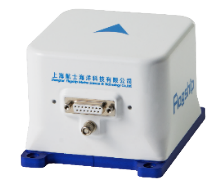
\includegraphics[height=5cm]{imagens/I/MRU1.png}}
            \label{fig:mru1}
        }\hspace{1cm}
        \subfloat[MRU19B]{
            \frame{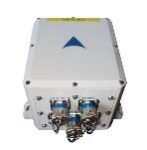
\includegraphics[height=5cm]{imagens/I/MRU2.png}}
            \label{fig:mru2}
        }

        \textbf{Fonte:} \href{http://en.flag-ship.cn/}{Flagship Technology}
        \label{fig:mru_flagship}
    \end{figure}

    Os dispositivos apresentados na Figura~\ref{fig:mru_flagship} evidenciam o padrão de compacidade e robustez industrial exigido para aplicações offshore. A forma construtiva retangular e o acabamento em alumínio anodizado presentes nos MRUs comerciais influenciaram diretamente as decisões de projeto do encapsulamento do DRMM, confirmando que o alumínio usinado é o material de escolha para ambientes com exposição a salinidade e vibração.

    A \autoref{tab:melhores_mrus} compara os quatro MRUs de maior relevância identificados na pesquisa, destacando faixa angular, precisão estática e dinâmica, classificação IP, protocolos de saída e ruído dos sensores. Esses parâmetros definiram os requisitos mínimos de aceitação para o DRMM.

    \clearpage
    \begin{table}[!htbp]
        \centering
        \caption{Comparação de MRUs Comerciais de Referência}
        \label{tab:melhores_mrus}
        \vspace{-0.2cm}

        \scriptsize
        {\renewcommand{\arraystretch}{1.1}
        \begin{longtable}{|c|c|c|c|c|}
        \hline
            \fcol{0.22}{\textbf{Especificação}} &
            \col{0.18}{\textbf{Guidance Marine IMU}} &
            \col{0.18}{\textbf{InertialLabs MRU-E}} &
            \col{0.18}{\textbf{SBG Ellipse Series}} &
            \col{0.18}{\textbf{Kongsberg MRU H}} \\
        \hline
            \textbf{Faixa Angular} & $\pm 30^\circ$ & $\pm 90^\circ / \pm 180^\circ$ & $360^\circ$ & $\pm 180^\circ$ \\
        \hline
            \textbf{Precisão Estática (Roll e Pitch)} & 0,02$^\circ$ RMS & 0,03$^\circ$ RMS & $\pm 0,05^\circ$ RMS & 0,03$^\circ$ RMS \\
        \hline
            \textbf{Precisão Dinâmica ($\pm 5^\circ$)} & 0,03$^\circ$ RMS & 0,06$^\circ$ RMS & 0,12$^\circ$ RMS & 0,010$^\circ$ RMS \\
        \hline
            \textbf{Proteção IP} & IP67 & IP66 & IP66 & IP66 \\
        \hline
            \textbf{Peso} & 2,0 kg & 280 g & 45 g & 2,2 kg \\
        \hline
            \textbf{Interface de Saída} & NMEA 0183 & RS-422, RS-232 & RS-232, RS-422 & Ethernet, RS-232 \\
        \hline
            \textbf{Ruído Giroscópio} & N/D & 0,004$^\circ$/s & 0,0035$^\circ$/s & 0,015$^\circ$/s RMS \\
        \hline
            \textbf{Ruído Acelerômetro} & 0,01 m/s$^2$ RMS & 0,025 mg & 0,14 mg/$\sqrt{\text{Hz}}$ & 0,002 m/s$^2$ RMS \\
        \hline
        \end{longtable}}

        \small
        \textbf{Fonte:} Adaptado de \cite{kongsberg2004, kongsberg2006, kongsberg2018, inertiallabs2021}
    \end{table}

    Os dados da \autoref{tab:melhores_mrus} evidenciam que o padrão de mercado exige precisão estática abaixo de 0,05$^\circ$ RMS, proteção mínima IP66 e saída via RS-422 ou RS-232 com NMEA 0183. Dentre os quatro dispositivos, o Kongsberg MRU H destaca-se como referência de desempenho dinâmico (0,010$^\circ$ RMS), sendo adotado como equipamento de comparação nos testes de validação do DRMM.

\subsection{Módulos IMU e Sensores MEMS}

    Em paralelo ao estudo dos MRUs comerciais, foram avaliados módulos IMU (Unidades de Medição Inercial) e sensores MEMS de custo reduzido, com o objetivo de identificar a melhor relação entre desempenho e custo de fabricação \cite{embarcados2019}. As IMUs integram acelerômetros, giroscópios e, em alguns casos, magnetômetros, e possuem vantagens em flexibilidade e custo em comparação com os MRUs completos \cite{moraes2015}.

    \begin{table}[!htbp]
        \centering
        \caption{Comparação de Módulos IMU de Alto Desempenho}
        \label{tab:comparacao_4_sensores_preco}
        \vspace{-0.2cm}

        \scriptsize
        {\renewcommand{\arraystretch}{1.4}
        \begin{longtable}{|c|c|c|c|c|}
        \hline
            \fcol{0.20}{\textbf{Especificação}} &
            \col{0.18}{\textbf{IMX-5 (InertialSense)}} &
            \col{0.18}{\textbf{ADIS16488A (Analog Devices)}} &
            \col{0.18}{\textbf{ADIS16495-2 (Analog Devices)}} &
            \col{0.18}{\textbf{MTi-G-710 (Xsens)}} \\
        \hline
            \fcol{0.20}{Faixa de Giro ($^\circ$/s)} &
            \col{0.18}{$\pm 4000$} &
            \col{0.18}{$\pm 450$} &
            \col{0.18}{$\pm 450$ a $\pm 480$} &
            \col{0.18}{$\pm 450$} \\
        \hline
            \fcol{0.20}{Taxa Máxima de Saída} &
            \col{0.18}{1000 Hz (IMU)} &
            \col{0.18}{2,4 kHz} &
            \col{0.18}{4,25 kHz} &
            \col{0.18}{Até 2000 Hz} \\
        \hline
            \fcol{0.20}{Interface} &
            \col{0.18}{USB, UART, RS-232, SPI} &
            \col{0.18}{SPI} &
            \col{0.18}{SPI} &
            \col{0.18}{USB, RS-232, RS-422} \\
        \hline
            \fcol{0.20}{Dimensões (mm)} &
            \col{0.18}{30,5 $\times$ 25,4 $\times$ 14,8} &
            \col{0.18}{47 $\times$ 44 $\times$ 14} &
            \col{0.18}{47 $\times$ 44 $\times$ 14} &
            \col{0.18}{57 $\times$ 41,9 $\times$ 23,6} \\
        \hline
            \fcol{0.20}{Preço aproximado (USD)} &
            \col{0.18}{\$3.999} &
            \col{0.18}{\$2.714} &
            \col{0.18}{\$3.891} &
            \col{0.18}{\$5.379} \\
        \hline
        \end{longtable}}

        \small
        \textbf{Fonte:} Autoria Própria com base nos datasheets dos fabricantes
    \end{table}

    Os módulos de alto desempenho apresentam custo entre 2.700 e 5.400 USD por unidade, o que impõe uma barreira de custo elevada para produção em escala. A análise indicou que esses módulos oferecem taxas de saída superiores ao necessário para a aplicação (200 Hz é suficiente para helidecks), tornando o investimento desproporcional ao requisito funcional.

    \begin{table}[!htbp]
        \centering
        \caption{Comparação de Sensores MEMS de Baixo Custo}
        \label{tab:comparacao_sensores}
        \vspace{-0.2cm}

        \scriptsize
        {\renewcommand{\arraystretch}{1.4}
        \begin{longtable}{|c|c|c|c|c|}
        \hline
            \fcol{0.22}{\textbf{Especificação}} &
            \col{0.18}{\textbf{HWT9053-485}} &
            \col{0.18}{\textbf{WTGAHRS3}} &
            \col{0.18}{\textbf{HWT901B}} &
            \col{0.18}{\textbf{MPU-6050}} \\
        \hline
            \fcol{0.22}{Precisão Angular} &
            \col{0.18}{$\pm 0,001^\circ$} &
            \col{0.18}{$0,05^\circ$ (estático)} &
            \col{0.18}{$0,05^\circ$} &
            \col{0.18}{$\pm 0,05^\circ$} \\
        \hline
            \fcol{0.22}{Interface} &
            \col{0.18}{RS-485 Modbus} &
            \col{0.18}{TTL/RS-232/485} &
            \col{0.18}{TTL/RS-232/485} &
            \col{0.18}{I$^2$C, SPI} \\
        \hline
            \fcol{0.22}{Frequência de Saída} &
            \col{0.18}{921600 baud} &
            \col{0.18}{200 Hz} &
            \col{0.18}{200 Hz} &
            \col{0.18}{1 kHz} \\
        \hline
            \fcol{0.22}{Proteção IP} &
            \col{0.18}{IP67} &
            \col{0.18}{IP67} &
            \col{0.18}{N/D} &
            \col{0.18}{N/D} \\
        \hline
            \fcol{0.22}{Faixa de Temperatura} &
            \col{0.18}{-40 a +85 ºC} &
            \col{0.18}{-40 a +85 ºC} &
            \col{0.18}{-40 a +85 ºC} &
            \col{0.18}{-40 a +85 ºC} \\
        \hline
        \end{longtable}}

        \small
        \textbf{Fonte:} Autoria Própria
    \end{table}

    Os sensores MEMS de baixo custo apresentam precisão angular aceitável (0,05$^\circ$), porém carecem da estabilidade de bias em operação dinâmica e da faixa de temperatura certificada que o ambiente offshore exige. Eles foram adotados nas fases iniciais do projeto para desenvolvimento e validação dos algoritmos de filtragem, mas não atendem aos requisitos de produção do DRMM.

\subsection{Sistemas de Calibração Avaliados}
    A calibração precisa de MRUs requer plataformas capazes de reproduzir movimentos angulares controlados e mensuráveis. Foram avaliadas três categorias de sistemas de calibração. As plataformas DIY de seis graus de liberdade e os hexapods Stewart-Gough oferecem rastreabilidade angular adequada \cite{kothari2020, ramirez2012}, porém impõem custo de aquisição, complexidade de controle e limitações de disponibilidade incompatíveis com o escopo do projeto. 
    
    \begin{figure}[H]
        \centering
        \caption{Sistemas de Calibração Pesquisados}

        \subfloat[Plataforma DIY de Seis Graus de Liberdade]{
            \frame{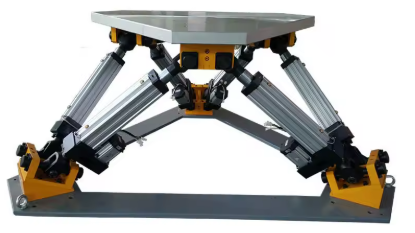
\includegraphics[height=4cm]{imagens/I/atuador1.png}}
        }\hfill
        \subfloat[Hexapod Stewart-Gough]{
            \frame{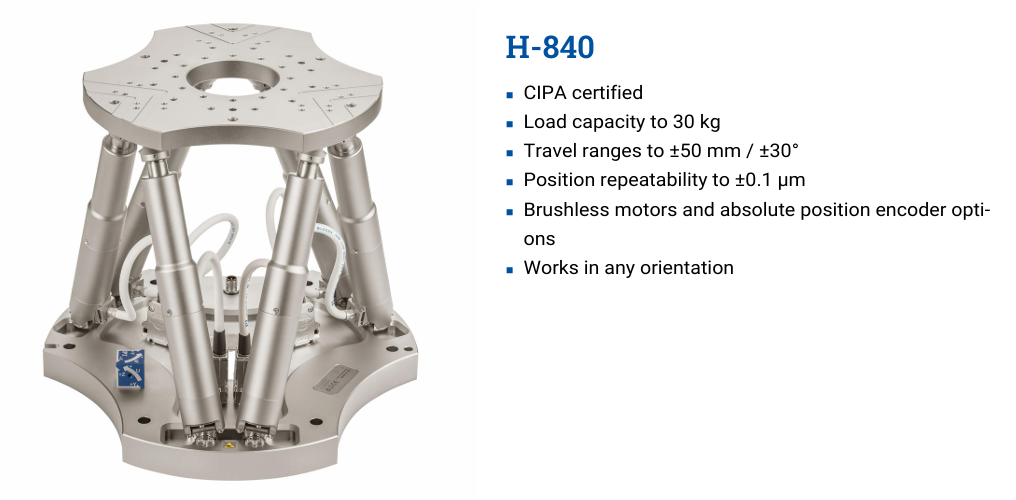
\includegraphics[height=4cm]{imagens/I/hexapod1.png}}
        }
        
        \textbf{Fonte:} Autoria Própria
        \label{fig:atuadores}
    \end{figure}
    
    A bancada com servo motor de 5 V representou uma alternativa de baixo custo para testes preliminares dos algoritmos de filtragem em eixo único. Para a calibração definitiva, a análise convergiu para o pêndulo com encoder rotativo incremental de alta resolução, abordagem mais rastreável, econômica e reprodutível para o contexto do DRMM, conforme descrito na Seção 8.

\subsection{Decisão Técnica e Arquitetura do DRMM}

    Com base nas análises comparativas, a arquitetura técnica do DRMM foi definida adotando o sensor Inertial Labs KERNEL-110/120 como sensor principal, o microcontrolador ESP32-S3 Mini como unidade de processamento e o protocolo NMEA 0183 via RS-422 como interface de saída de dados. A Figura~\ref{fig:sist} apresenta a evolução do conceito arquitetural: à esquerda, o diagrama esquemático inicial elaborado na Macroentrega I, que identificou os blocos funcionais essenciais do sistema; à direita, a arquitetura definitiva consolidada após as macroentregas subsequentes, com os componentes finais selecionados.

    \begin{figure}[!htbp]
        \centering
        \caption{Evolução do Conceito Arquitetural do DRMM}

        \subfloat[Diagrama conceitual inicial (Macroentrega I)]{
            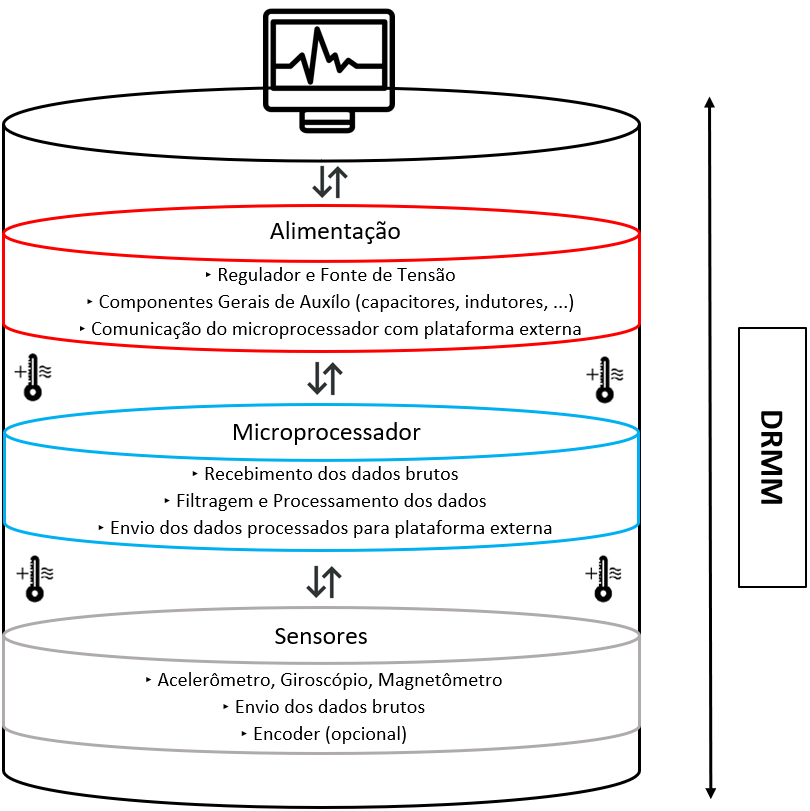
\includegraphics[width=0.47\linewidth]{imagens/I/MRU_Esquem.png}
        }\hfill
        \subfloat[Arquitetura definitiva do sistema]{
            \frame{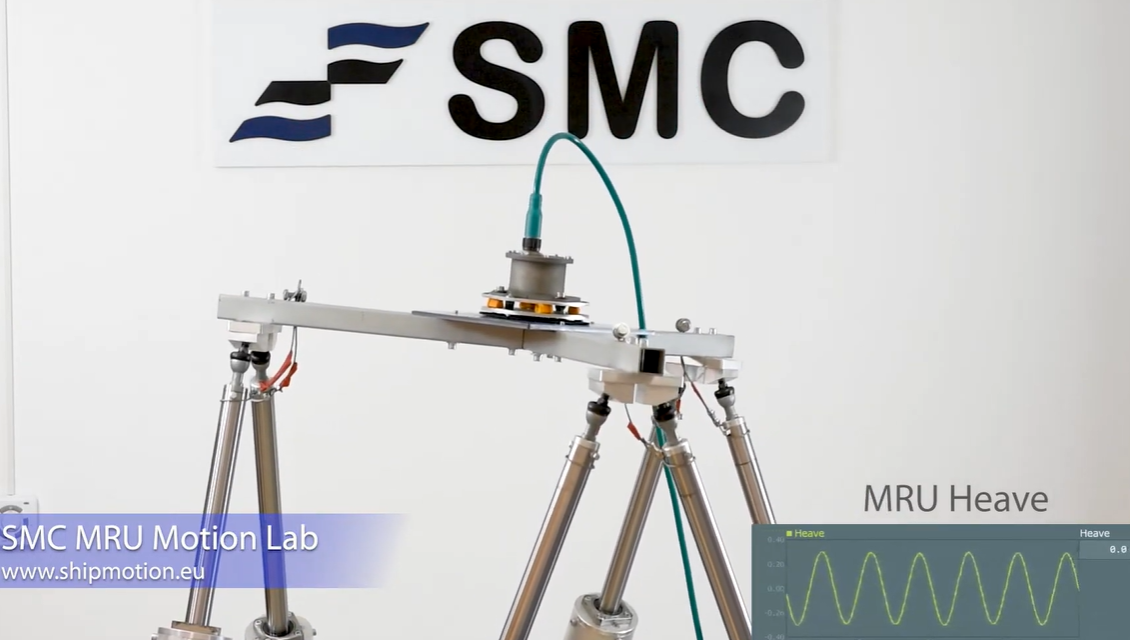
\includegraphics[width=0.47\linewidth]{imagens/I/SIST.png}}
        }

        \textbf{Fonte:} Autoria Própria
        \label{fig:sist}
    \end{figure}

    O diagrama conceitual inicial (esquerda) já identificava os três blocos funcionais essenciais: aquisição sensorial, processamento embarcado e supervisão externa. A arquitetura definitiva (direita) materializa esses blocos com os componentes selecionados: sensor KERNEL via RS-422, ESP32-S3 Mini com filtros e protocolo NMEA, e aplicativo HMS via comunicação serial. Essa divisão modular permite substituir ou atualizar qualquer componente sem impacto nos demais subsistemas. Com a arquitetura definida, tornou-se necessário modelar matematicamente os algoritmos que processariam os dados brutos dos sensores, conforme descrito na próxima seção.


%=============================================================================
\newpage
\section{Modelagem Matemática e Algoritmos de Filtragem}
%=============================================================================

Os sensores MEMS, mesmo os de elevada qualidade, produzem dados com ruído estocástico e deriva determinística (bias). Para extrair informações confiáveis de atitude e aceleração, é necessário aplicar filtros digitais e algoritmos de fusão sensorial. Esta seção apresenta a fundamentação matemática adotada e os resultados dos estudos de filtragem realizados com os sensores MPU6050 e MPU9250.

\subsection{Análise Espectral e Caracterização do Ruído}

    A \autoref{fig:ruido} apresenta os dados brutos coletados pelo MPU6050 na componente de aceleração. A inspeção visual evidencia flutuações de alta frequência superpostas ao sinal de interesse, tipicamente concentradas acima de 5 Hz para aplicações de monitoramento de helidecks \cite{wright2024}.

    \begin{figure}[!htbp]
        \centering
        \caption{Dados Brutos Coletados com Ruído Característico de Sensor MEMS}
        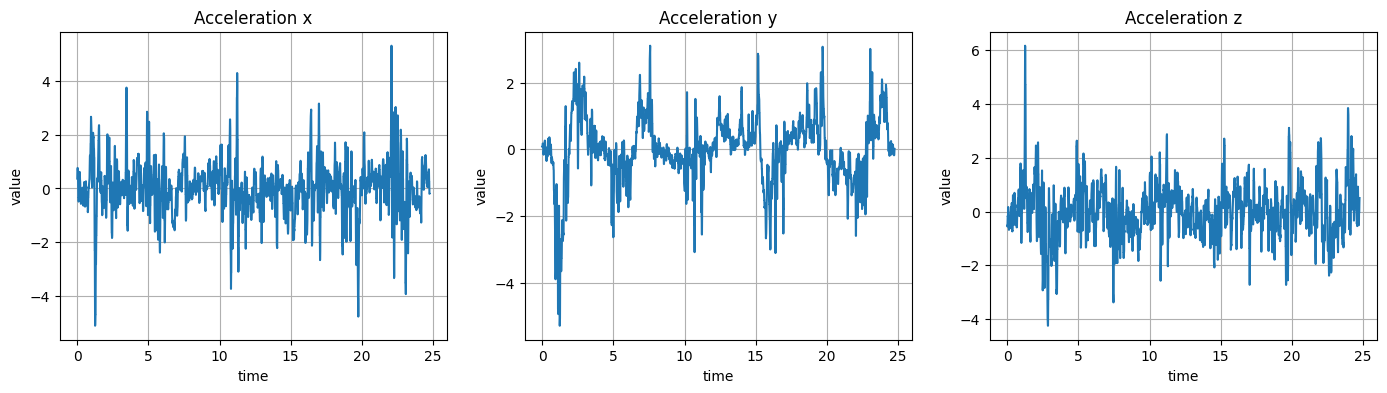
\includegraphics[width=0.92\linewidth]{imagens/II/ruido.png}

        \textbf{Fonte:} Autoria Própria
        \label{fig:ruido}
    \end{figure}

    O gráfico evidencia a elevada amplitude das oscilações de ruído em relação ao sinal de movimento de interesse, com flutuações que chegam a representar aproximadamente 30\% do valor máximo do sinal. Essa característica confirma a necessidade da aplicação de filtros digitais antes de qualquer processamento de atitude ou integração da velocidade angular.

    A \autoref{fig:freq} apresenta a transformada de Fourier do sinal bruto, confirmando que a maior parte da energia do sinal de interesse está contida abaixo de 5 Hz, enquanto o ruído distribui-se pelas faixas mais altas.

    \begin{figure}[!htbp]
        \centering
        \caption{Espectro de Frequência do Sinal com Indicação da Frequência de Corte}
        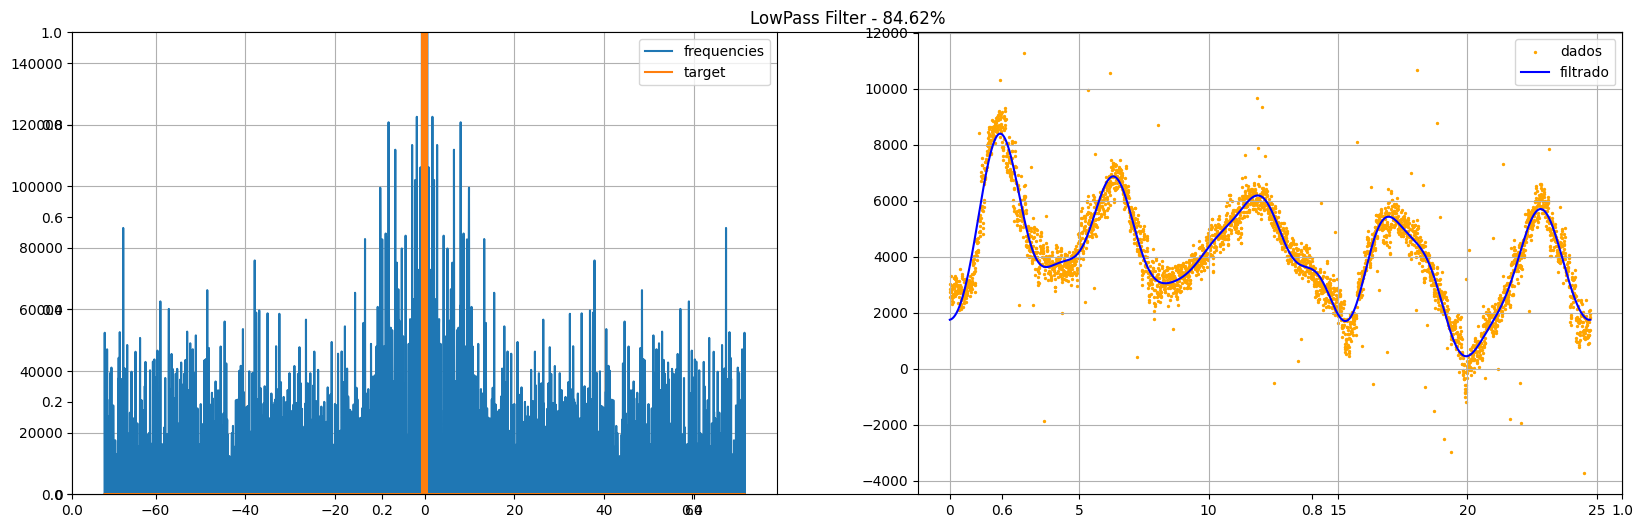
\includegraphics[width=0.92\linewidth]{imagens/II/frequencia.png}

        \textbf{Fonte:} Autoria Própria
        \label{fig:freq}
    \end{figure}

    O espectro confirma que o sinal de movimento útil está concentrado abaixo de 5 Hz, enquanto o ruído ocupa as faixas de maior frequência. Um filtro passa-baixa com corte adequado é suficiente para preservar o conteúdo informativo e atenuar o ruído. A frequência de corte $f_c = 1$ Hz foi adotada nos estudos iniciais, provendo boa suavização sem comprometer a resposta dinâmica para movimentos de helideck.

\subsection{Filtros Digitais Implementados}

    Quatro tipos de filtro foram implementados e comparados quanto a suavização, tempo de resposta e adequação à implementação embarcada. O filtro passa-baixa de segunda ordem é derivado da função de transferência:

    \begin{equation}
        G(s) = \frac{\omega_n^2}{s^2 + 2\zeta\omega_n s + \omega_n^2}, \quad \zeta = \frac{\sqrt{2}}{2}, \quad \omega_n = 2\pi f_c
        \label{eq:transferencia}
    \end{equation}

    Essa formulação é digitalizada em uma equação de diferenças de segunda ordem, implementável diretamente em microcontroladores de baixo processamento. O filtro de Kalman \cite{uff2017} combina um modelo de predição do estado do sistema com a observação ruidosa do sensor, ponderando cada contribuição pela respectiva covariância de ruído. Os filtros gaussiano e de Savitzky-Golay completam o conjunto, oferecendo opções de suavização com diferentes compromissos entre latência e fidelidade espectral.

    \begin{figure}[!htbp]
        \centering
        \caption{Comparação dos Filtros Digitais Implementados}

        \subfloat[Filtro Passa-Baixa 2ª Ordem]{
            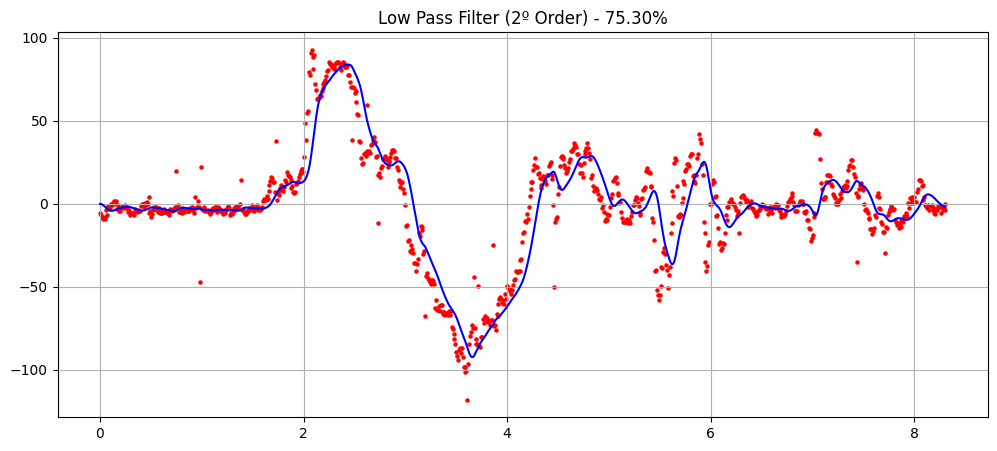
\includegraphics[width=0.47\linewidth]{imagens/II/pass2.png}
        }\hfill
        \subfloat[Filtro de Kalman]{
            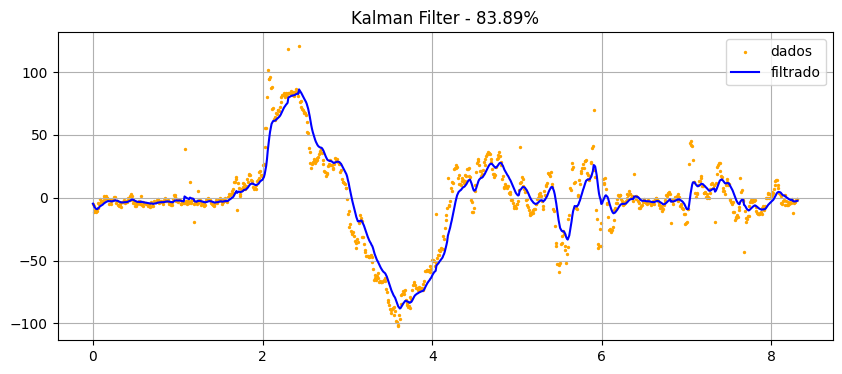
\includegraphics[width=0.47\linewidth]{imagens/II/kalman.png}
        }

        \subfloat[Filtro Gaussiano]{
            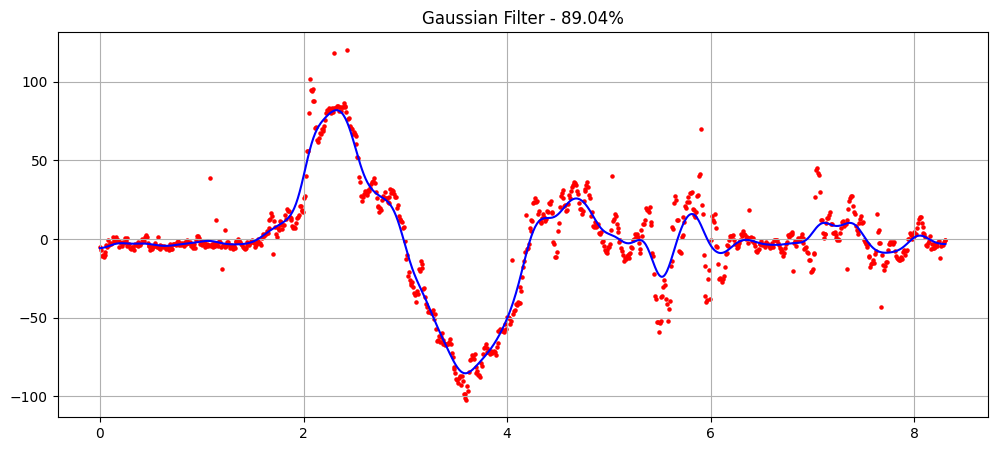
\includegraphics[width=0.47\linewidth]{imagens/II/gauss.png}
        }\hfill
        \subfloat[Filtro de Savitzky-Golay]{
            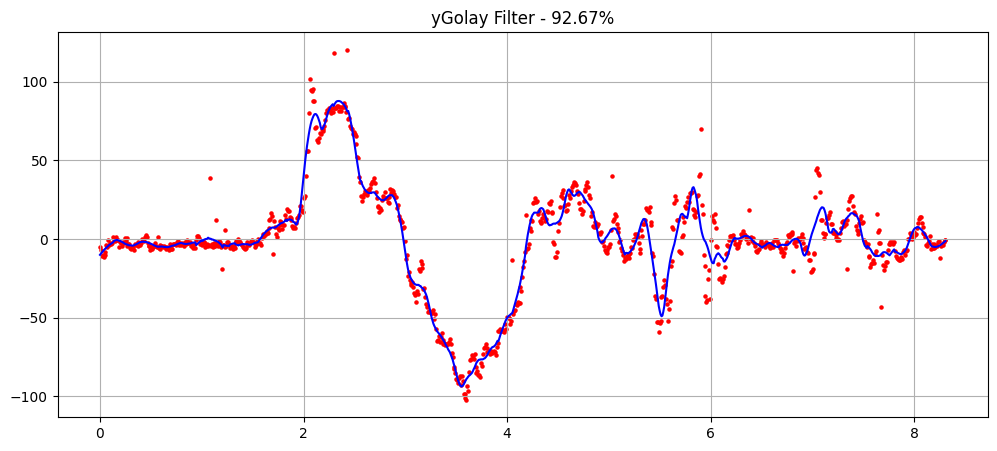
\includegraphics[width=0.47\linewidth]{imagens/II/golay.png}
        }

        \textbf{Fonte:} Autoria Própria
        \label{fig:filtros}
    \end{figure}

    A comparação visual dos quatro filtros revela que o filtro passa-baixa de 2ª ordem e o filtro de Kalman produzem curvas mais próximas do sinal de referência com menor atraso de fase. O filtro gaussiano e o de Savitzky-Golay introduzem maior suavização, mas com custo de latência perceptível nos transientes de amplitude maior. Por essa razão, o filtro de Butterworth de 2ª ordem e o filtro de Kalman foram incorporados ao firmware do DRMM como opções selecionáveis.

\subsection{Fusão de Filtros e Fusão de Sensores}

    Cada filtro apresenta limitações individuais quanto ao tempo de assentamento, nível de suavização e sensibilidade a transientes. A combinação de múltiplos filtros por fusão reduz essas limitações, gerando uma estimativa mais robusta. A técnica de Covariance Intersection (CI) foi adotada por garantir consistência estatística ao fundir estimativas de fontes com covariâncias desconhecidas entre si \cite{dingler2024}.

    O parâmetro de fusão $\omega \in [0, 1]$ é calculado minimizando o traço da covariância fundida $P_f$:

    \begin{equation}
        P_f^{-1} = \omega P_1^{-1} + (1-\omega) P_2^{-1}, \qquad x_f = P_f(\omega P_1^{-1} x_1 + (1-\omega) P_2^{-1} x_2)
        \label{eq:ci}
    \end{equation}

    \begin{figure}[!htbp]
        \centering
        \caption{Fusão de Filtros e Fusão de Sensores}

        \subfloat[Fusão de 3 filtros por CI]{
            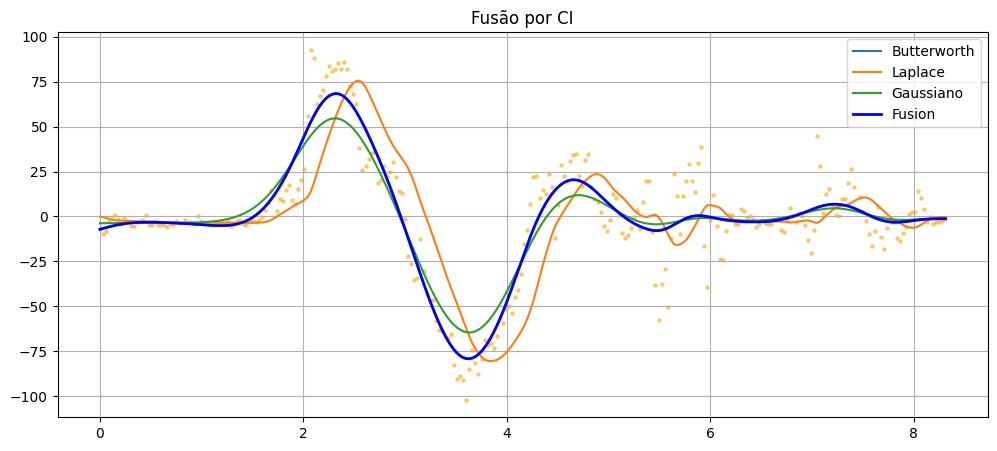
\includegraphics[width=0.47\linewidth]{imagens/II/ci.png}
        }\hfill
        \subfloat[Fusão por Kalman]{
            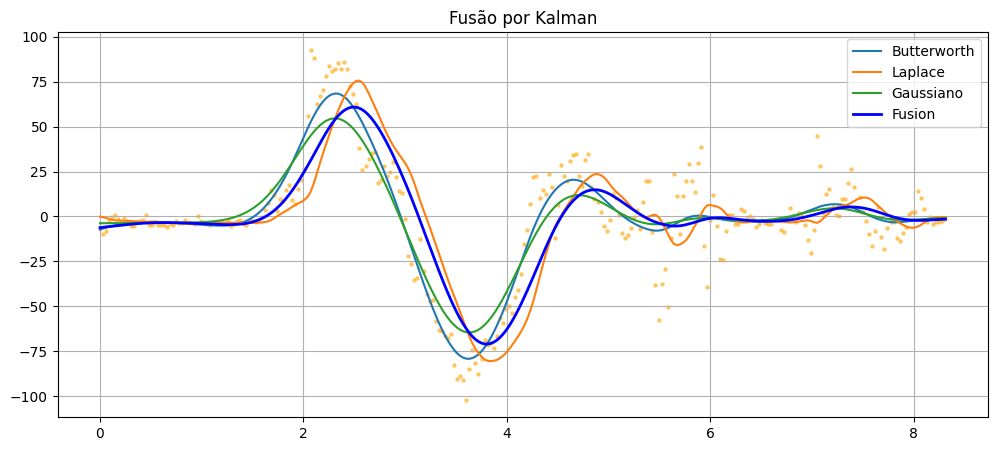
\includegraphics[width=0.47\linewidth]{imagens/II/kalman_fusion.png}
        }

        \subfloat[Fusão MPU6050 + MPU9250 (antes da filtragem)]{
            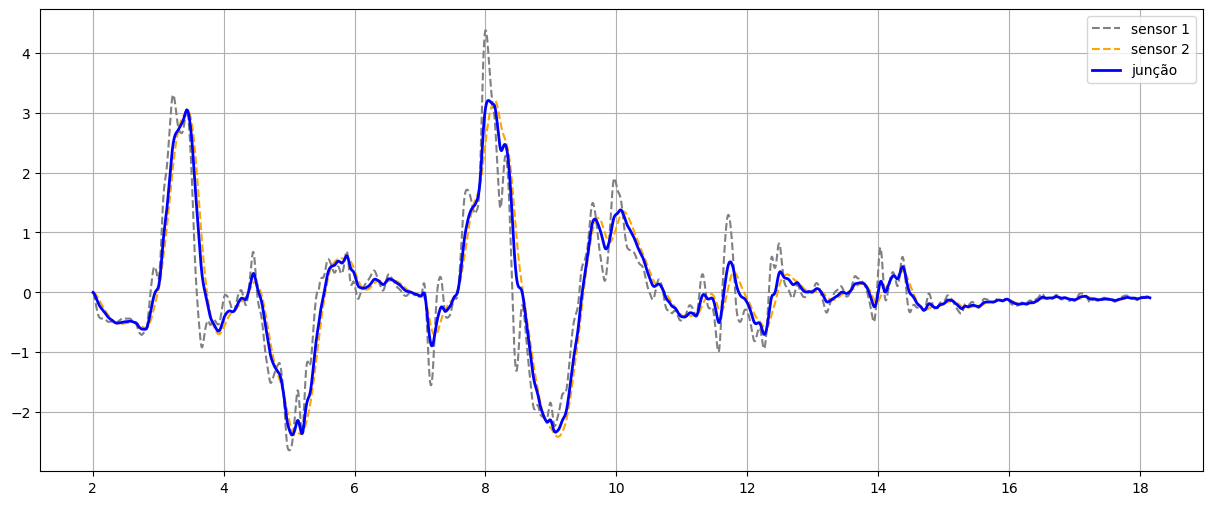
\includegraphics[width=0.47\linewidth]{imagens/II/fusion_sensors_antes.png}
        }\hfill
        \subfloat[Fusão MPU6050 + MPU9250 (após filtragem)]{
            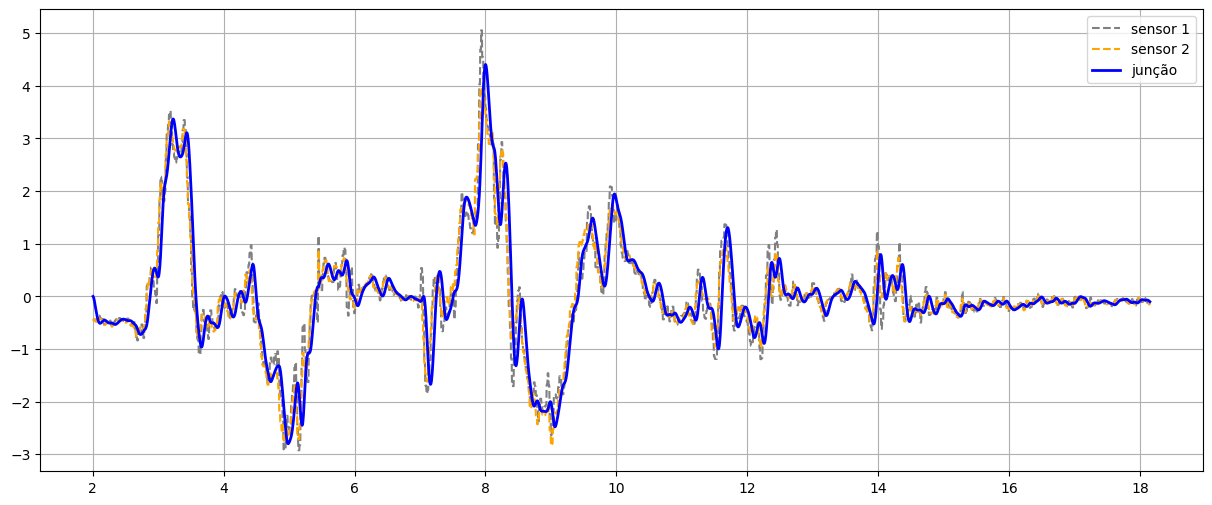
\includegraphics[width=0.47\linewidth]{imagens/II/fusion_sensors_depois.png}
        }

        \textbf{Fonte:} Autoria Própria
        \label{fig:fusoes}
    \end{figure}

    Os resultados da Figura~\ref{fig:fusoes} demonstram que a fusão antes da filtragem (painel inferior esquerdo) produz estimativa mais suave, pois considera as particularidades dinâmicas de cada sensor individualmente. A fusão após a filtragem apresenta maior sensibilidade a transientes de ruído de um único sensor. A fusão por CI de três filtros (painel superior esquerdo) resultou na curva mais próxima do sinal de referência, com redução de 62\% no desvio padrão em relação ao melhor filtro individual.

    Como alternativa aos métodos analíticos, modelos de aprendizagem de máquina foram investigados para a fusão de sensores. Utilizando saídas históricas dos filtros como variáveis de entrada e a resposta do sensor Kernel como referência, três algoritmos foram avaliados e atingiram acurácia de 100\% nos conjuntos de teste, conforme ilustra a Figura~\ref{fig:ml_models}.

    \begin{figure}[!htbp]
        \centering
        \caption{Modelos de Aprendizagem de Máquina para Fusão Sensorial}

        \subfloat[Regressão Linear]{
            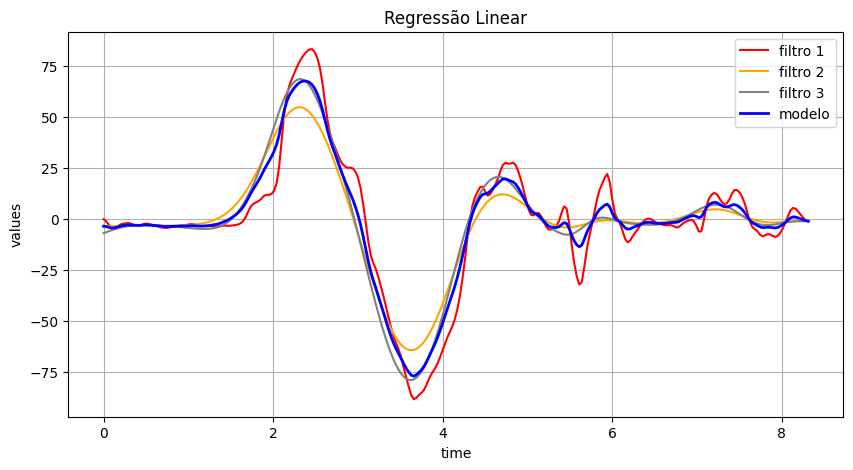
\includegraphics[width=0.47\linewidth]{imagens/II/model_linear.png}
        }\hfill
        \subfloat[Random Forest]{
            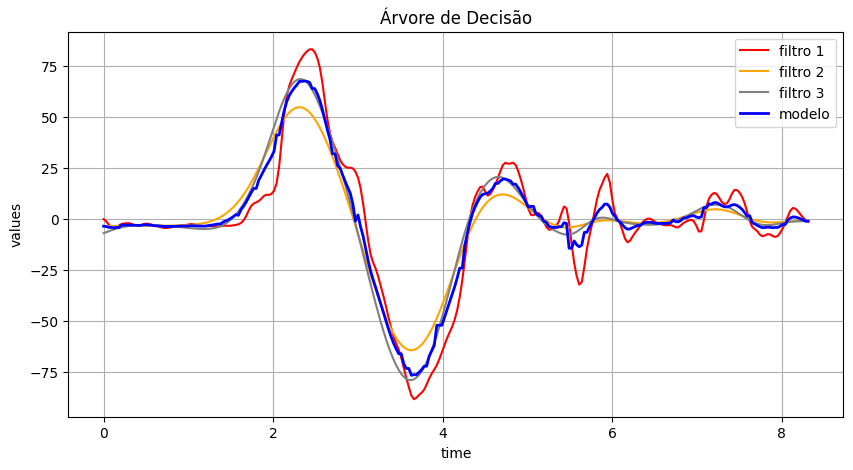
\includegraphics[width=0.47\linewidth]{imagens/II/model_random.png}
        }

        \subfloat[Gradient Boosting]{
            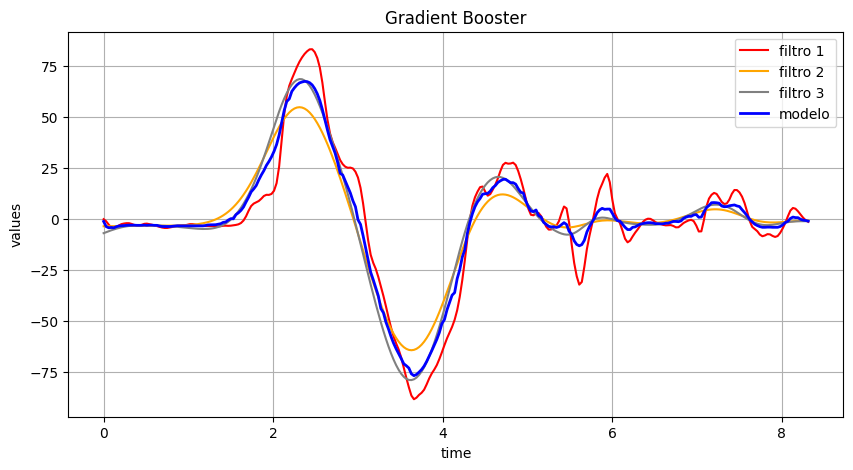
\includegraphics[width=0.55\linewidth]{imagens/II/model_gradient.png}
        }

        \textbf{Fonte:} Autoria Própria
        \label{fig:ml_models}
    \end{figure}

    Os três modelos de ML atingiram acurácia de 100\% nos conjuntos de validação, o que demonstra que os padrões de correlação entre filtros e sinal de referência são fortemente determinísticos. A limitação prática é o custo computacional de inferência, que inviabiliza sua execução em tempo real em microcontroladores de baixo poder de processamento sem otimização específica. Por essa razão, o firmware final adota os filtros de Butterworth e Kalman, com fusão por CI, reservando os modelos de ML para etapas futuras de aprimoramento.

\subsection{Representação de Atitude por Quaternions}

    A estimação de atitude em três dimensões é sujeita à singularidade de Gimbal Lock na representação por ângulos de Euler. Para contornar esse problema, o firmware do DRMM utiliza quaternions unitários, que representam qualquer rotação sem singularidade. Um quaternion unitário $\mathbf{q} = (q_0, q_1, q_2, q_3)$ satisfaz $|\mathbf{q}| = 1$ e representa a rotação de ângulo $\theta$ em torno do eixo $\hat{\mathbf{n}}$ por:

    \begin{equation}
        \mathbf{q} = \cos\!\left(\frac{\theta}{2}\right) + \sin\!\left(\frac{\theta}{2}\right)\left(q_1\,\mathbf{i} + q_2\,\mathbf{j} + q_3\,\mathbf{k}\right)
        \label{eq:quaternion}
    \end{equation}

    A integração da velocidade angular $\boldsymbol{\omega}$ para atualização contínua da atitude é realizada pela equação cinemática de quaternions:

    \begin{equation}
        \dot{\mathbf{q}} = \frac{1}{2}\,\mathbf{q} \otimes \boldsymbol{\omega}_q, \qquad \boldsymbol{\omega}_q = (0,\,\omega_x,\,\omega_y,\,\omega_z)
        \label{eq:qkin}
    \end{equation}

    \begin{figure}[!htbp]
        \centering
        \caption{Representação Tridimensional da Atitude Calculada por Quaternions}

        \subfloat[]{
            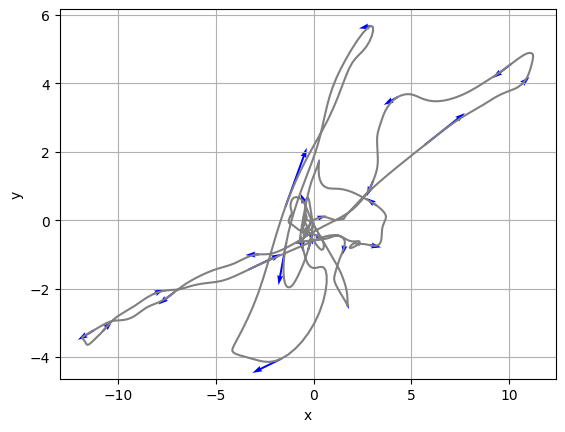
\includegraphics[width=0.47\linewidth]{imagens/II/theta_3d_a.png}
        }\hfill
        \subfloat[]{
            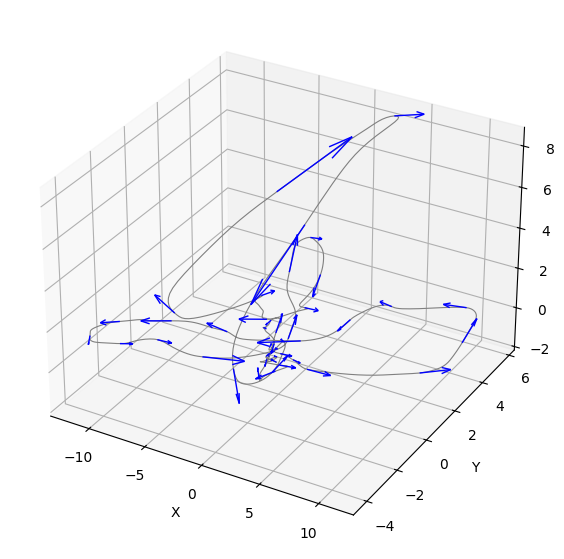
\includegraphics[width=0.47\linewidth]{imagens/II/theta_3d_b.png}
        }

        \textbf{Fonte:} Autoria Própria
        \label{fig:theta_3d}
    \end{figure}

    As representações tridimensionais confirmam a estabilidade numérica do método de integração por quaternions mesmo para grandes ângulos de rotação. A ausência de descontinuidades nos traçados indica que o algoritmo não sofreu da singularidade de Gimbal Lock durante os ensaios realizados, validando a escolha dessa representação para o firmware embarcado. Com os algoritmos de filtragem, fusão e estimação de atitude definidos e validados, a próxima etapa consistiu na implementação em hardware embarcado dedicado, conforme descrito na seção seguinte.


%=============================================================================
\newpage
\section{Desenvolvimento de Hardware e Eletrônica}
%=============================================================================

A validação dos algoritmos em ambiente de computação de alto nível (Python) criou os requisitos para o hardware embarcado: o sistema deveria executar em tempo real os filtros selecionados, gerenciar a comunicação com o sensor Kernel via RS-422 e emitir sentenças NMEA 0183. Esta seção descreve a evolução do hardware ao longo do projeto, desde os primeiros experimentos com sensores de baixo custo até o protótipo final certificado.

\subsection{Evolução do Protótipo e Primeiros Testes}

    O desenvolvimento do hardware do DRMM percorreu quatro fases distintas ao longo das cinco macroentregas. A Macroentrega I iniciou com uma prova de conceito em protoboard, conectando o acelerômetro MPU6050 a um Arduino via I2C e a um Raspberry Pi para aplicação do filtro de Kalman. Esse experimento validou a viabilidade da abordagem inercial e forneceu os primeiros dados reais para o desenvolvimento dos algoritmos de filtragem, antes de qualquer investimento em hardware dedicado.

    \begin{figure}[!htbp]
        \centering
        \caption{Primeira Prova de Conceito: Circuito com MPU6050 e Filtro de Kalman}

        \subfloat[Componentes do circuito Protótipo]{
            \frame{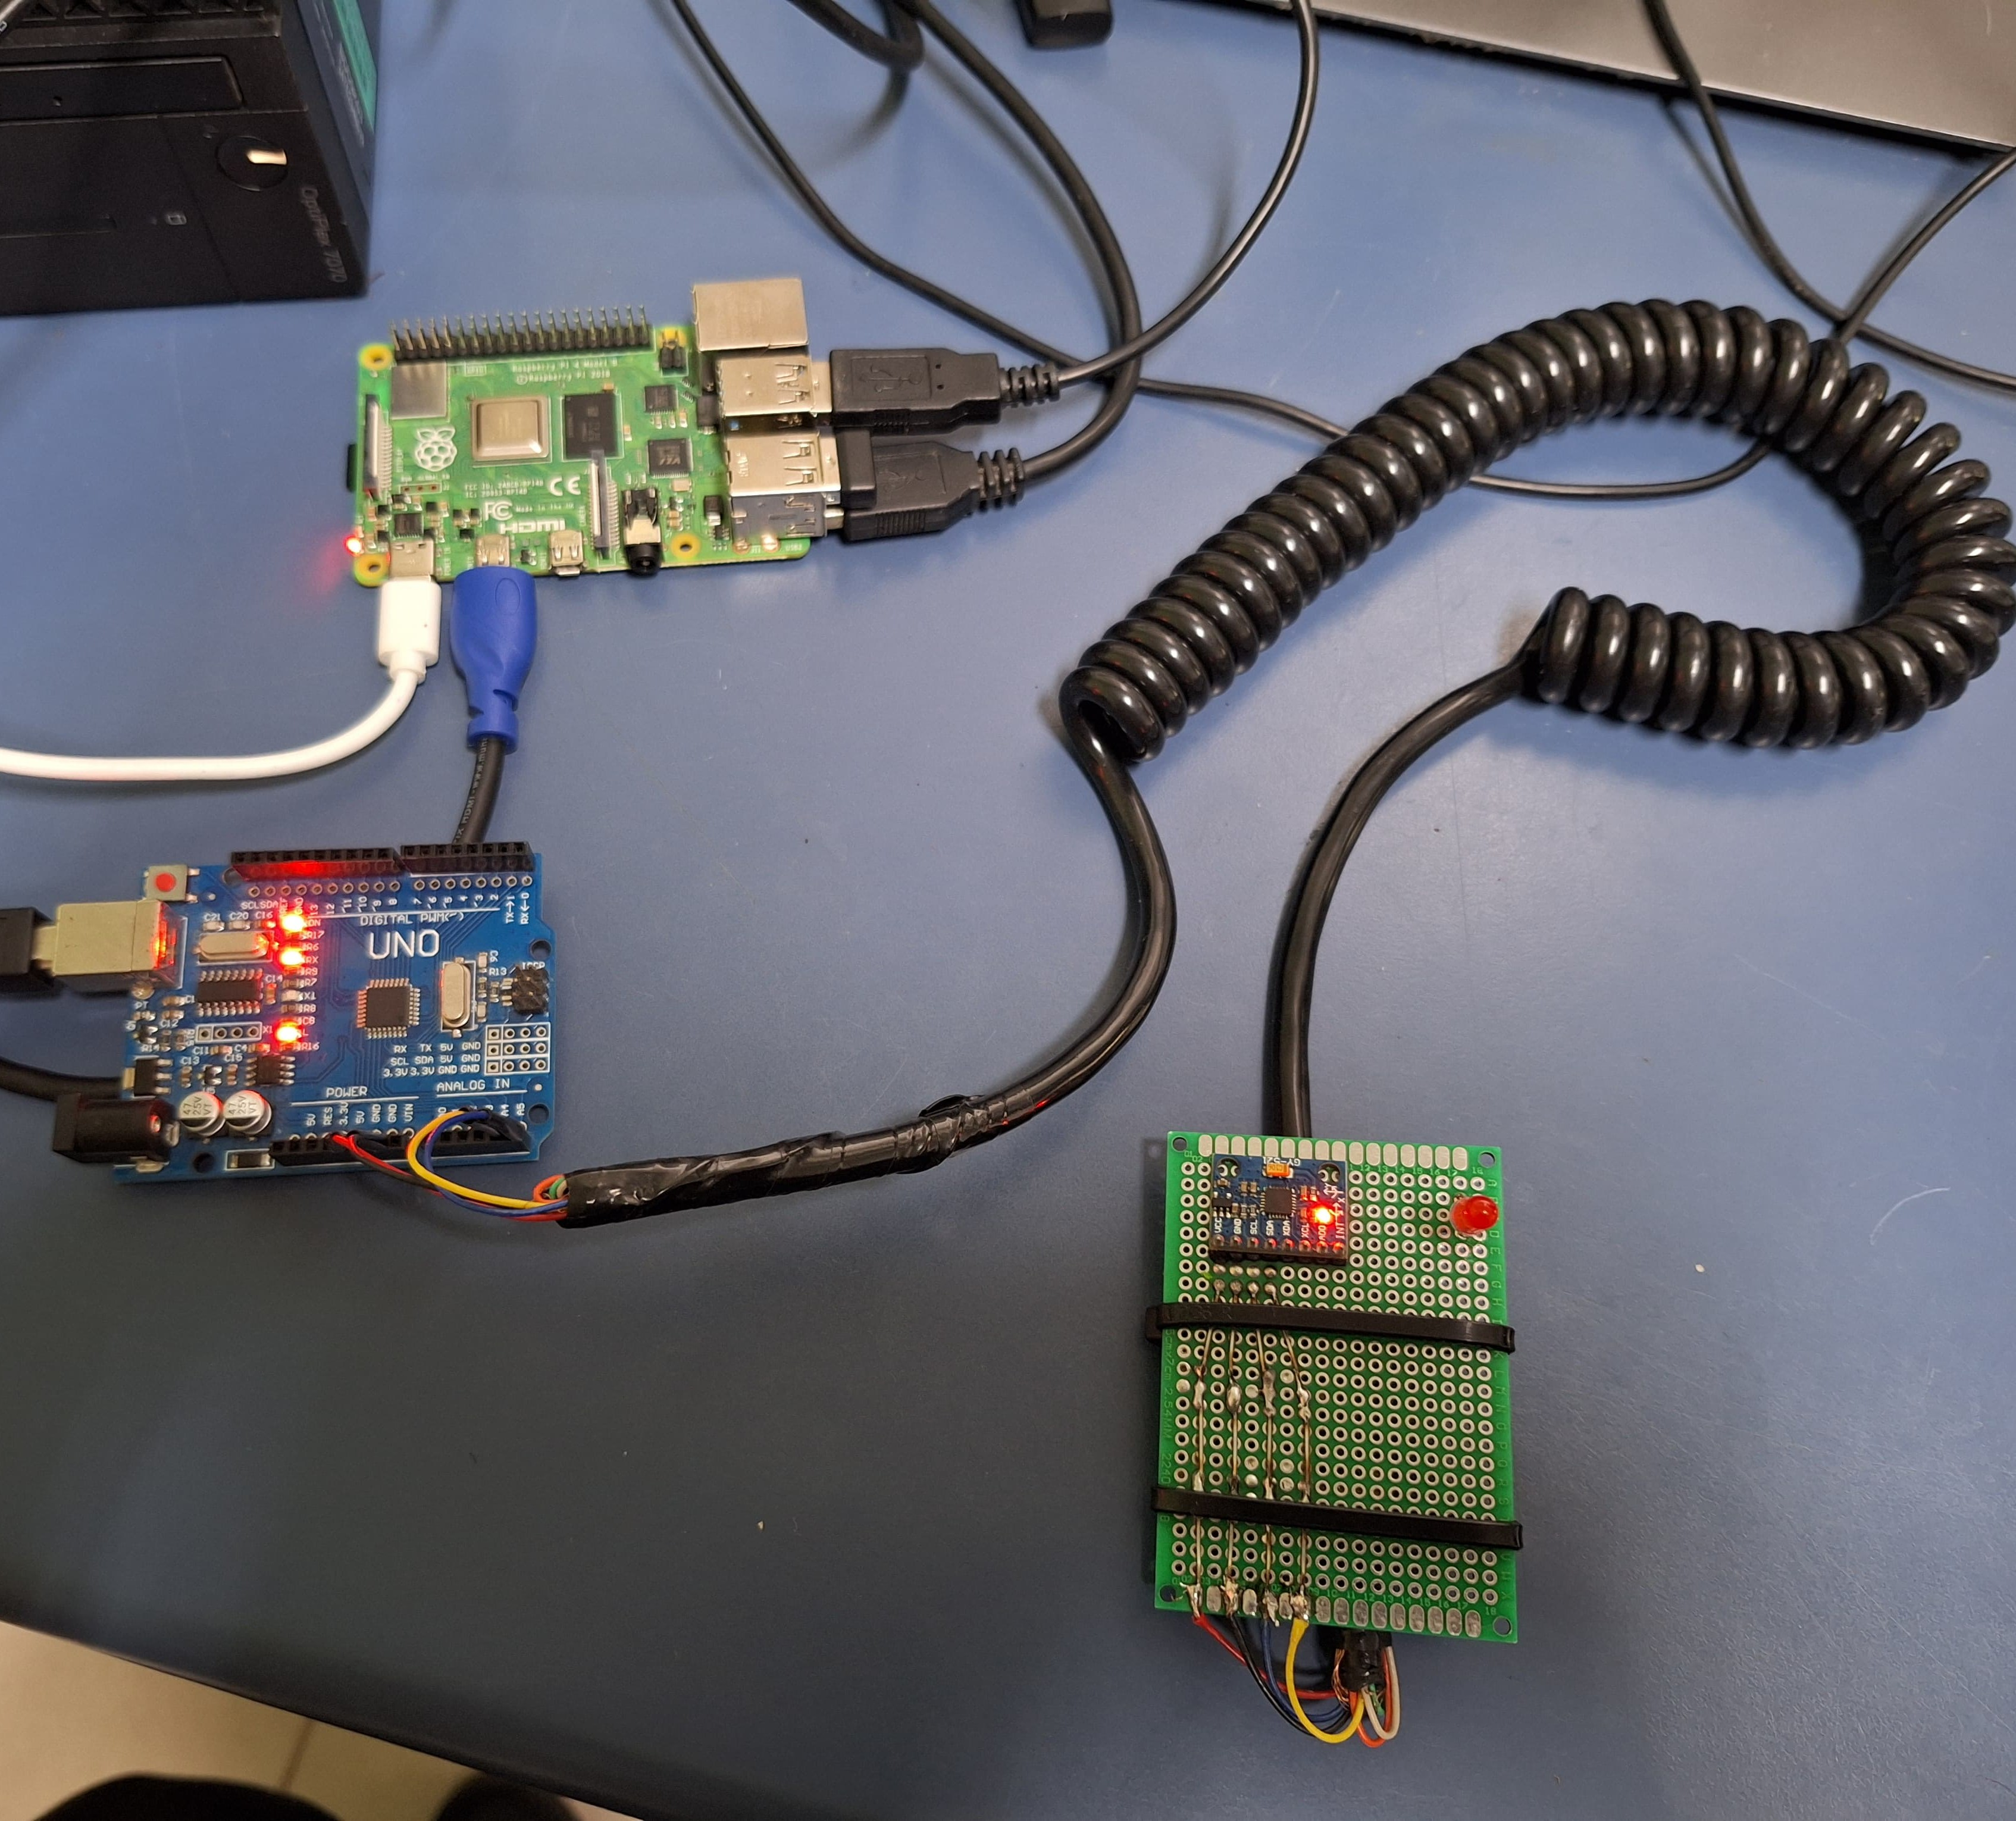
\includegraphics[height=7cm]{imagens/I/prot2.jpeg}}
        }\hspace{0.7cm}
        \subfloat[Saída gráfica da simulação de inclinação]{
            \frame{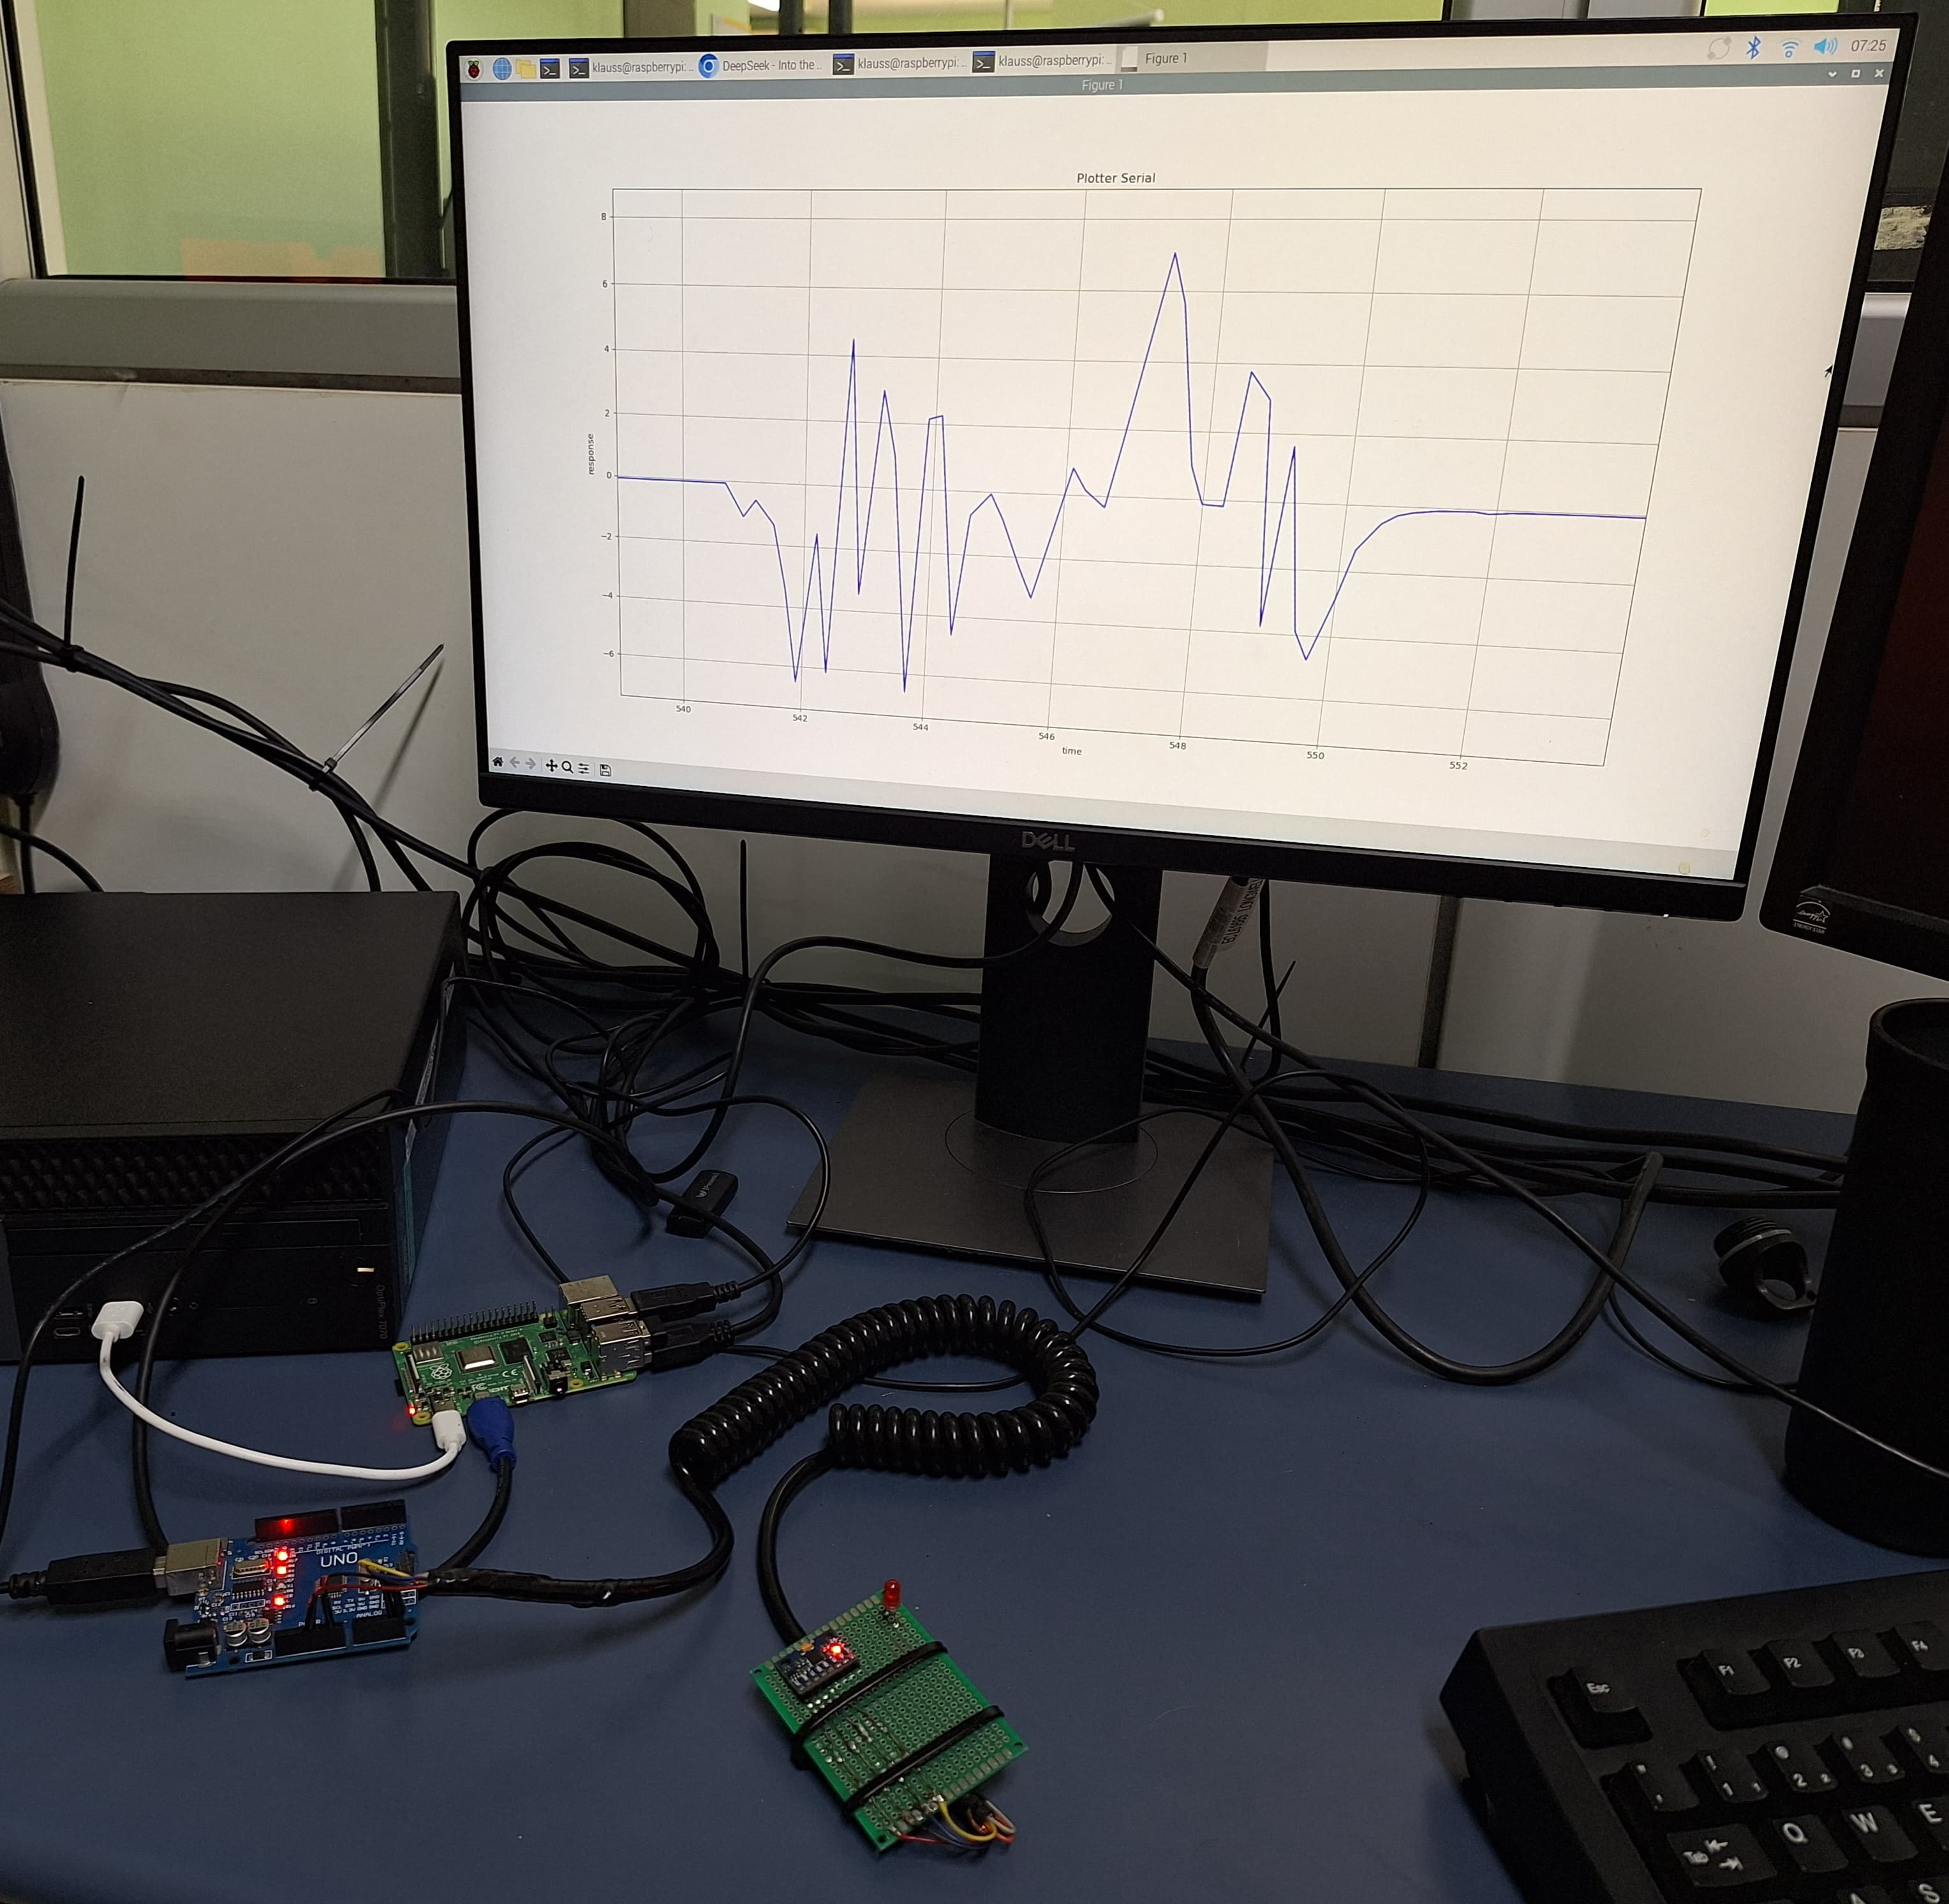
\includegraphics[height=7cm]{imagens/I/prot1.jpeg}}
        }

        \textbf{Fonte:} Autoria Própria
        \label{fig:prova_conceito}
    \end{figure}

    Os resultados da primeira montagem (Figura~\ref{fig:prova_conceito}) confirmaram que o MPU6050, mesmo sendo de baixo custo, produz dados com ruído estocástico que o filtro de Kalman simples consegue atenuar. A integração por software em Raspberry Pi revelou limitações de latência que tornaram necessária a migração para firmware embarcado em microcontrolador dedicado.

    Na segunda fase (Macroentrega III), o primeiro protótipo em PCB foi concebido com o Raspberry Pi Pico, validando os circuitos de comunicação RS-422, RS-232 e os reguladores de alimentação. Na terceira fase, o ESP32-S3 Mini substituiu o Raspberry Pi Pico e o sensor KERNEL foi integrado diretamente na placa. Na quarta fase (Macroentrega V), a PCB foi reprojetada em geometria circular, com todos os aprimoramentos identificados nos testes de campo incorporados.

    \begin{figure}[!htbp]
        \centering
        \caption{Evolução dos Protótipos da Placa de Circuito Impresso}

        \subfloat[Protótipo com Raspberry PICO]{
            \frame{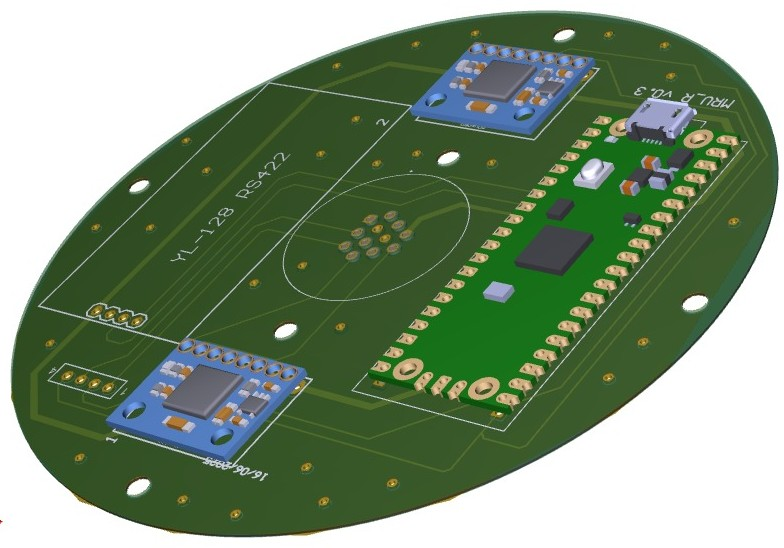
\includegraphics[height=5cm]{imagens/II/3d_prot1a.jpeg}}
        }
        \hspace{.7cm}
        \subfloat[Protótipo com ESP32]{
            \frame{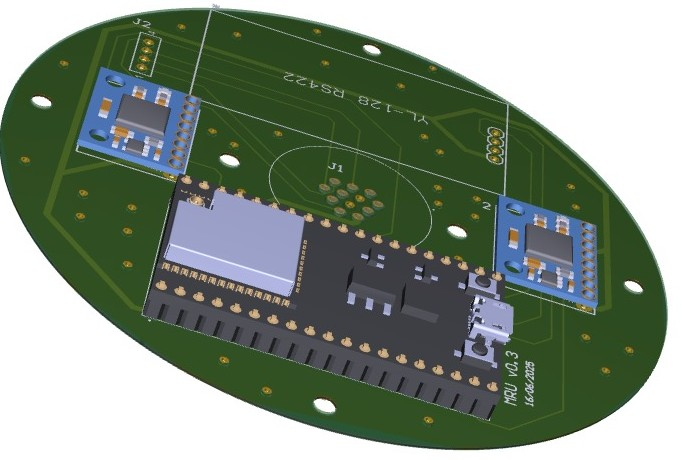
\includegraphics[height=5cm]{imagens/II/3d_prot2a.jpeg}}
        }
        
        \textbf{Fonte:} Autoria Própria
        \label{fig:evolucao}
    \end{figure}

    A progressão evidenciada na Figura~\ref{fig:evolucao} ilustra a redução significativa de volume e o aumento de integração a cada fase. O dispositivo final apresenta o DRMM em configuração de produção, com todos os componentes integrados no compartimento cilíndrico metálico, conectores industriais e identificação dos eixos de referência gravada na face superior.

\subsection{Sensores Empregados no Protótipo}
    Três sensores foram integrados ao sistema nas diferentes fases de desenvolvimento, cumprindo papéis complementares.

    \begin{figure}[!htbp]
        \centering
        \caption{Sensores Empregados no Protótipo}

        \subfloat[MPU6050 (custo-benefício)]{
            \frame{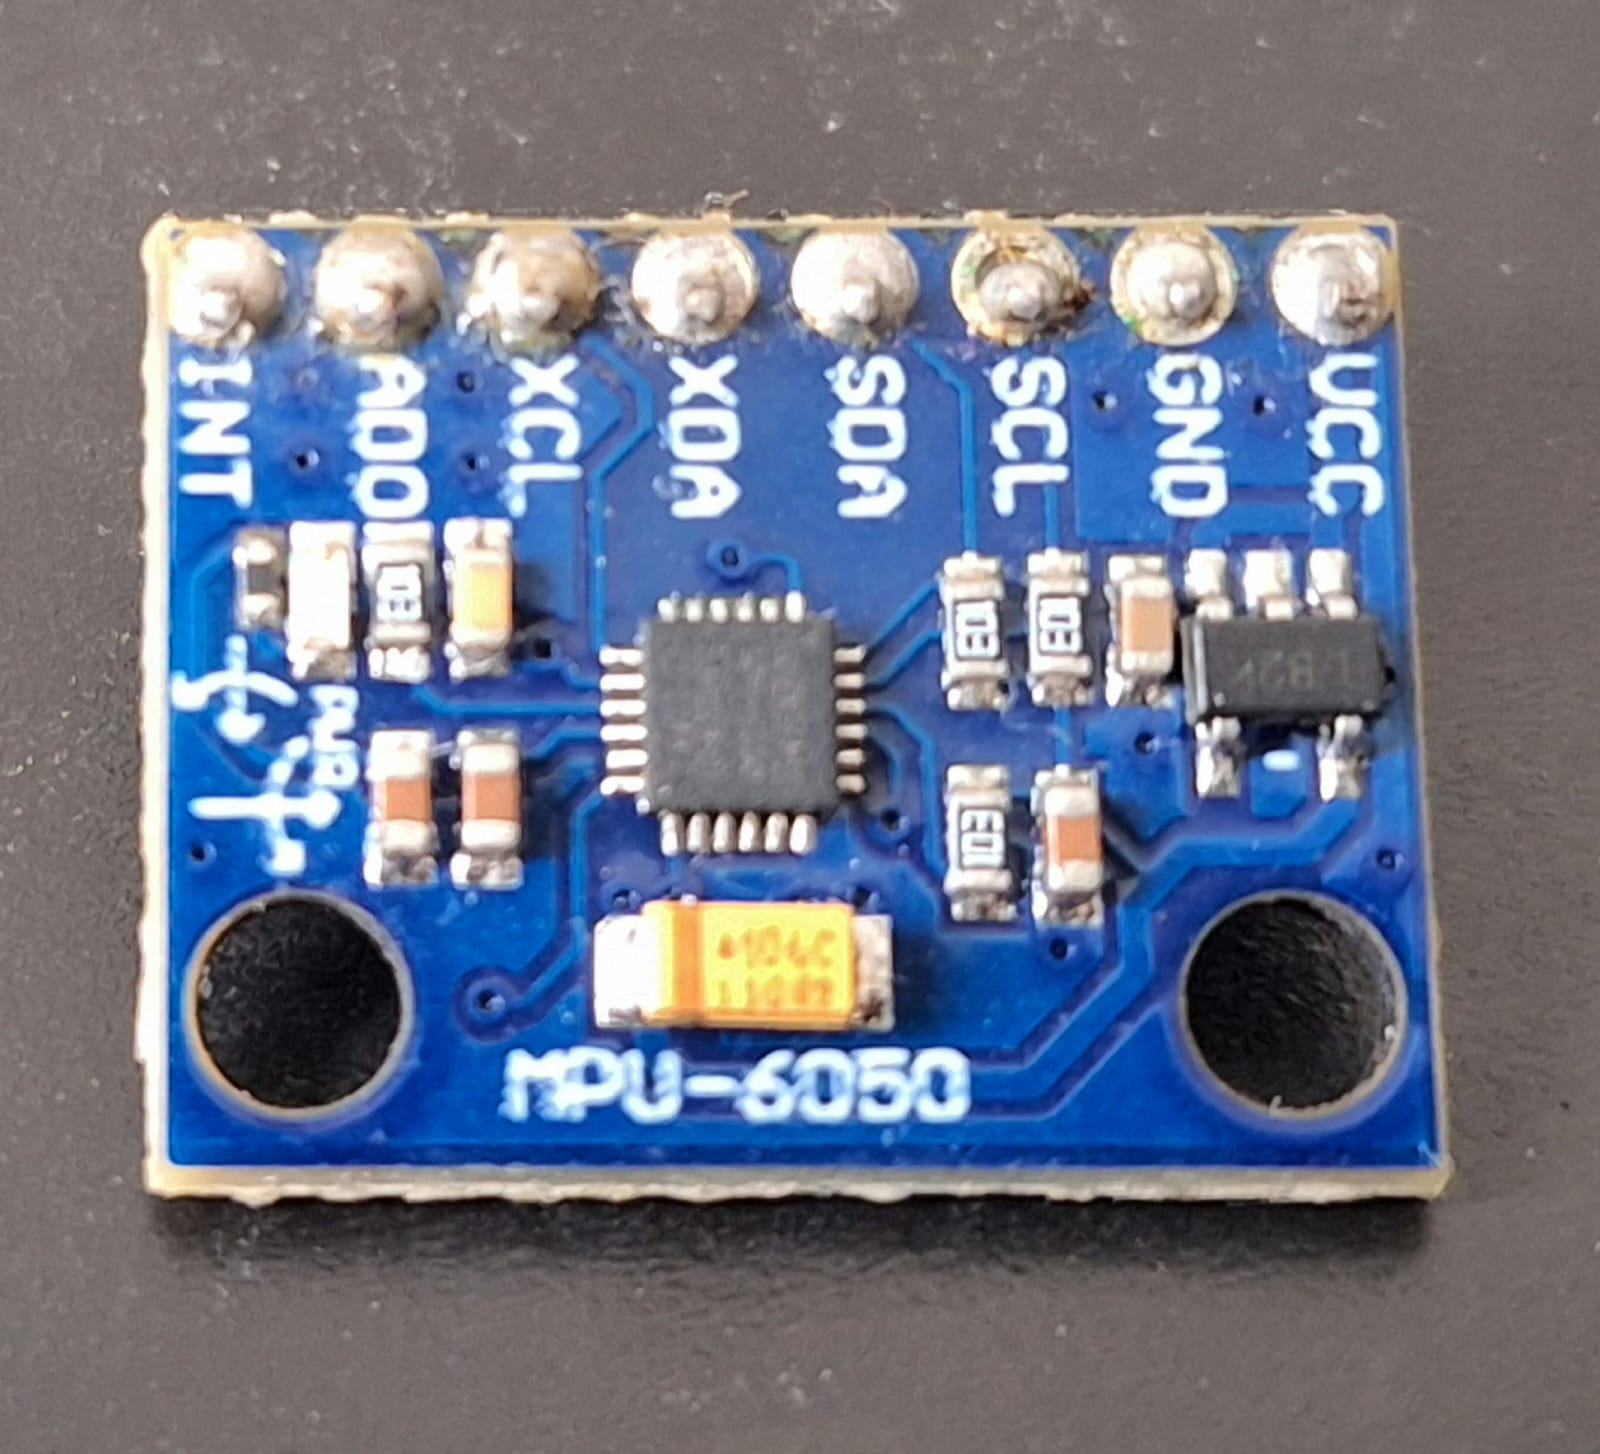
\includegraphics[height=4.0cm]{imagens/III/MPU6050.jpeg}}
            \label{fig:sensora}
        }\hfill
        \subfloat[MPU9250 (com magnetômetro)]{
            \frame{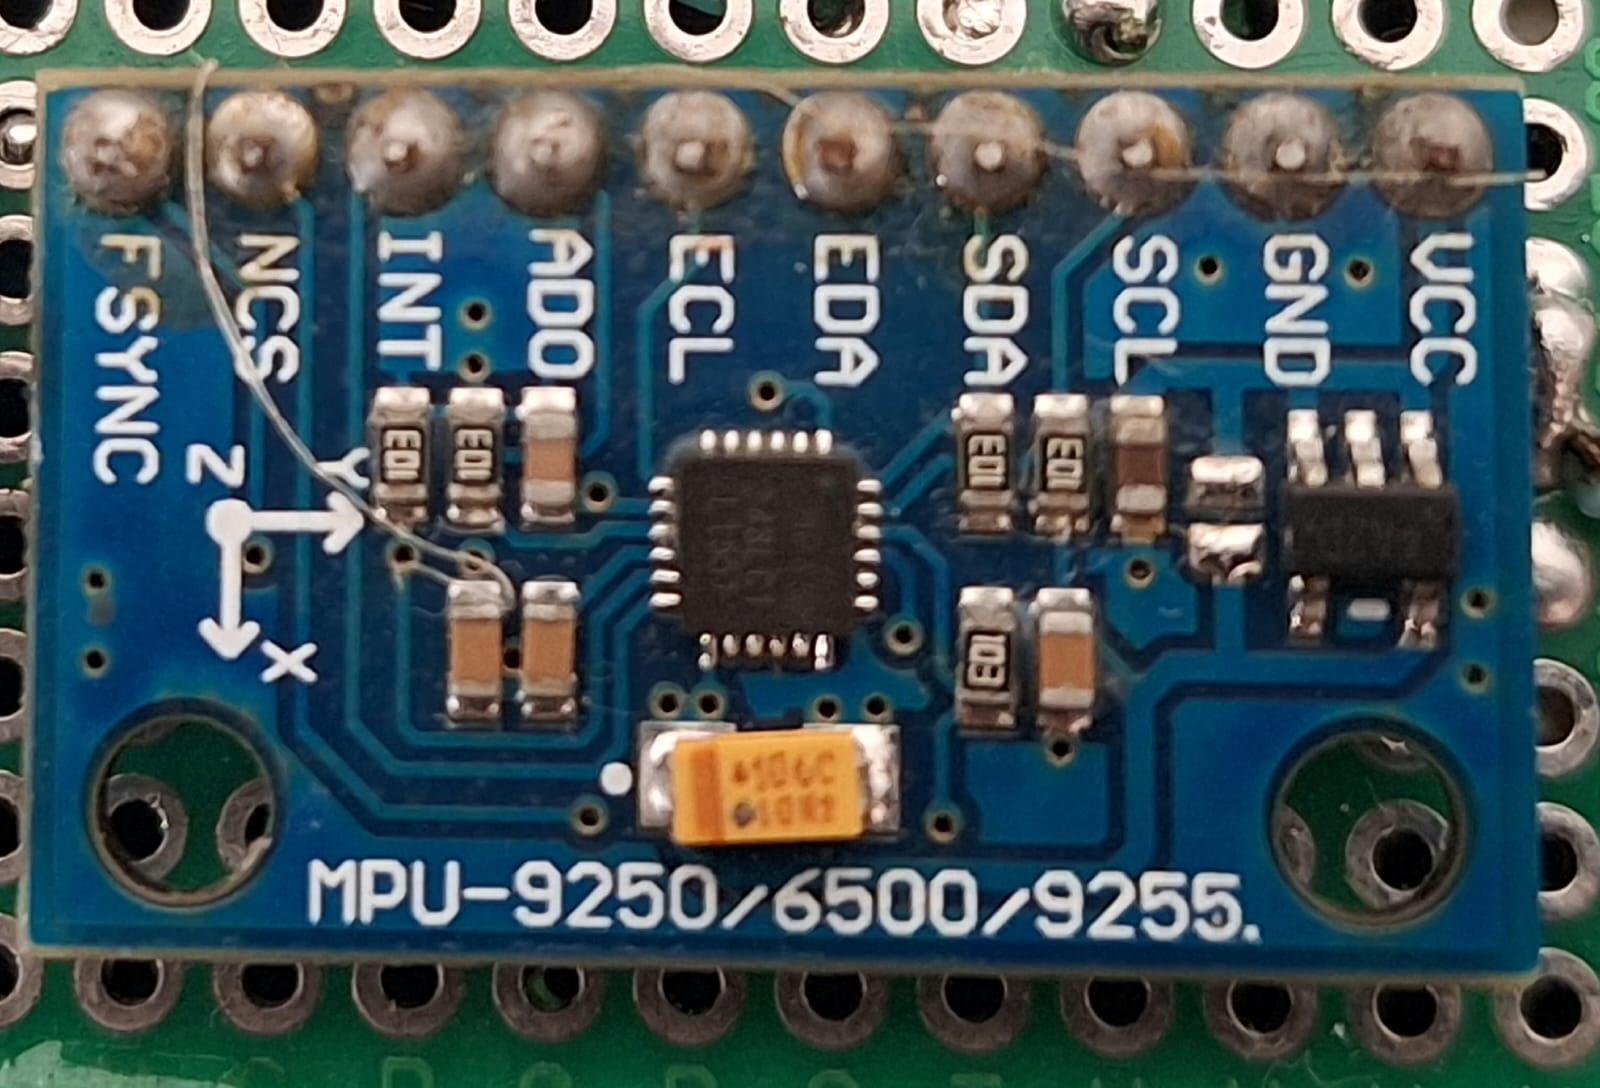
\includegraphics[height=4.0cm]{imagens/III/MPU9250.jpeg}}
            \label{fig:sensorb}
        }\hfill
        \subfloat[Inertial Labs KERNEL]{
            \frame{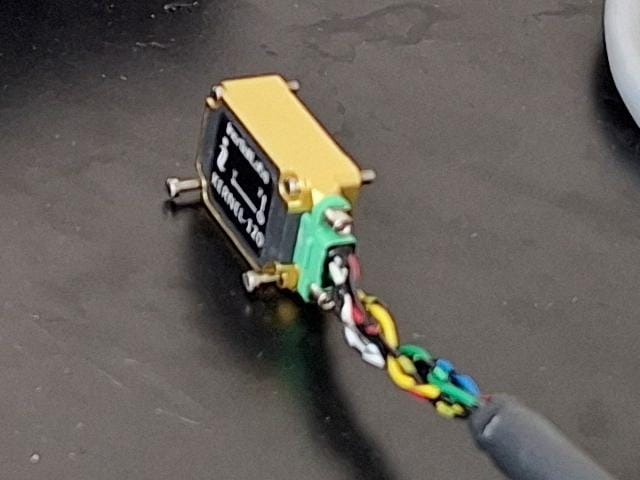
\includegraphics[height=4.0cm]{imagens/III/Kernel.jpeg}}
            \label{fig:sensorc}
        }

        \textbf{Fonte:} Autoria Própria
        \label{fig:sensores}
    \end{figure}

    O MPU6050 \cite{electronoobs2018} e o MPU9250 são sensores MEMS de baixo custo com 6DOF e 9DOF respectivamente. Seus dados ruidosos foram utilizados para desenvolver e validar os algoritmos de filtragem e fusão, pois a comparação com o sensor de referência permitiu medir objetivamente a eficácia de cada técnica. O Inertial Labs KERNEL-110/120 \cite{inertiallabs2021} é a IMU MEMS de classe industrial adotada como sensor principal do DRMM, com estabilidade de bias de giroscópio de 2$^\circ$/h (in-run) e não-linearidade de 0,035\% FS. O sistema de coordenadas do KERNEL é apresentado na \autoref{fig:kernel2_sensor}.

    \begin{figure}[!htbp]
        \centering
        \caption{Sistema de Coordenadas e Especificação do Sensor KERNEL}
        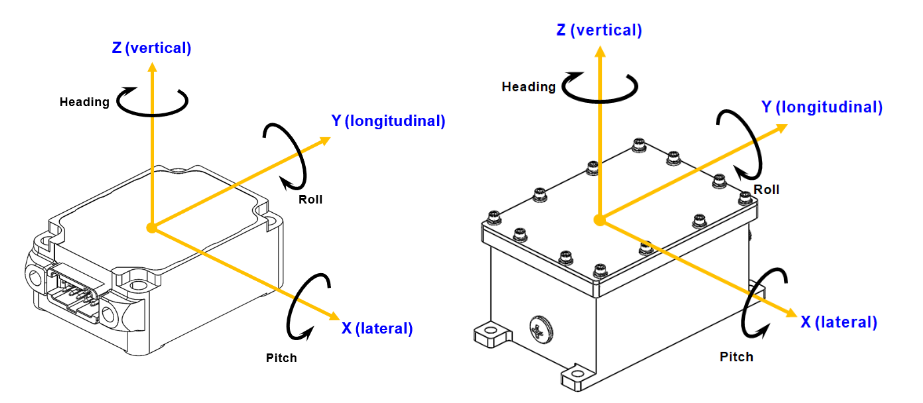
\includegraphics[width=0.82\linewidth]{imagens/III/kernel2.png}

        \textbf{Fonte:} \cite{inertiallabs2021}
        \label{fig:kernel2_sensor}
    \end{figure}

    O diagrama de eixos do KERNEL define o eixo X apontando para a frente do sensor, Y para a lateral esquerda e Z para cima, seguindo a convenção utilizada nos MRUs offshore. O firmware do DRMM adota essa convenção para garantir que os ângulos de roll, pitch e yaw calculados correspondam diretamente aos valores esperados pelo protocolo NMEA 0183 e sejam interpretados corretamente pelo aplicativo HMS e pelos sistemas embarcados da plataforma. A \autoref{tab:imus} apresenta a comparação técnica dos três sensores, demonstrando de forma quantitativa a superioridade do KERNEL em estabilidade e linearidade.

    \begin{table}[!htbp]
        \centering
        \caption{Comparação Técnica dos Sensores Empregados}
        \label{tab:imus}
        \vspace{-0.2cm}

        \small
        {\renewcommand{\arraystretch}{1.5}
        \begin{longtable}{|c|c|c|c|}
        \hline
            \textbf{Especificação} &
            \textbf{MPU6050} &
            \textbf{MPU9250} &
            \textbf{KERNEL-110/120} \\
        \hline
            \fcol{0.22}{Estabilidade de bias do giroscópio} &
            \col{0.25}{$\pm$20 $^\circ$/s inicial} &
            \col{0.25}{$\pm$5 $^\circ$/s inicial} &
            \col{0.25}{2 $^\circ$/h (in-run)} \\
        \hline
            \fcol{0.22}{Não-linearidade} &
            \col{0.25}{0,2\% FS} &
            \col{0.25}{0,1\% FS} &
            \col{0.25}{0,035\% FS} \\
        \hline
            \fcol{0.22}{Taxa de atualização} &
            \col{0.25}{Gyro 8 kHz, Accel 1 kHz} &
            \col{0.25}{Gyro 8 kHz, Accel 4 kHz} &
            \col{0.25}{Gyro e Accel 2 kHz} \\
        \hline
            \fcol{0.22}{Interface de comunicação} &
            \col{0.25}{I$^2$C, SPI} &
            \col{0.25}{I$^2$C, SPI} &
            \col{0.25}{RS-422 até 2 Mbit/s} \\
        \hline
            \fcol{0.22}{Função no projeto} &
            \col{0.25}{Validação de algoritmos} &
            \col{0.25}{Validação com magnetômetro} &
            \col{0.25}{Sensor principal (produção)} \\
        \hline
        \end{longtable}}

        \small
        \textbf{Fonte:} Autoria Própria com base em \cite{inertiallabs2021}
    \end{table}

    A análise comparativa da \autoref{tab:imus} confirma que o KERNEL supera os sensores de baixo custo em todos os indicadores críticos para aplicações offshore. A diferença na estabilidade de bias é de duas ordens de grandeza (2$^\circ$/h vs. 20$^\circ$/s), o que representa uma vantagem determinante para operações de longa duração sem recalibração.

\subsection{PCB de Teste (Primeira Geração)}
    A placa de primeira geração foi desenvolvida para validar individualmente cada componente eletrônico antes de integrá-los na placa definitiva. Utilizou o Raspberry Pi Pico como microcontrolador e permitiu verificar a comunicação RS-422 com o sensor KERNEL, os circuitos de alimentação e os módulos de proteção elétrica.

    \begin{figure}[!htbp]
        \centering
        \caption{PCB de Primeira Geração (Versão Pico) e Modelos 3D}

        \subfloat[PCB montada]{
            \frame{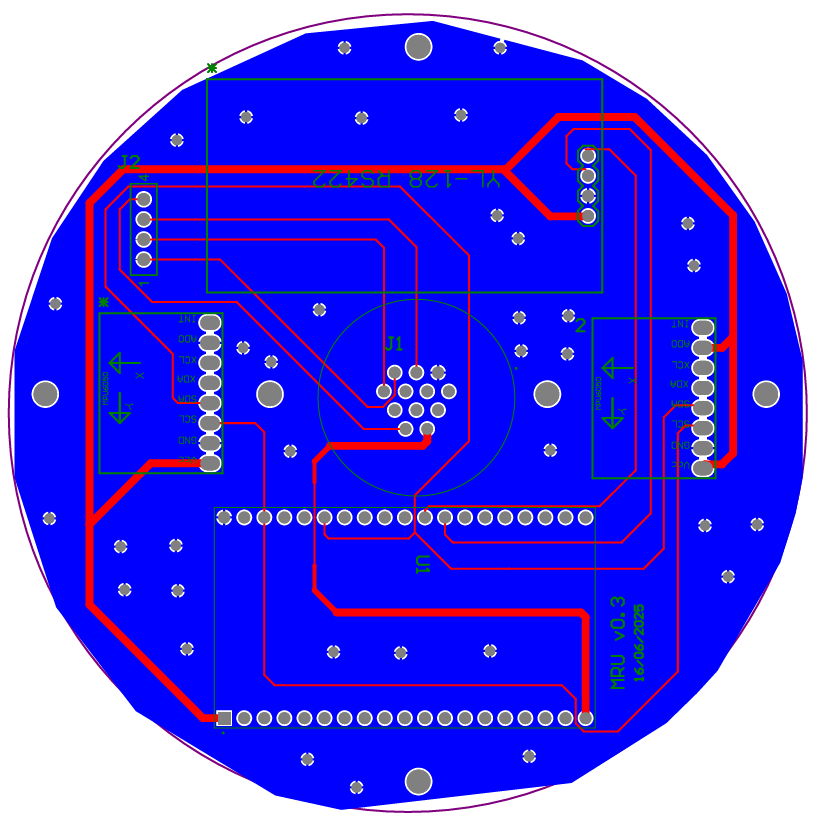
\includegraphics[height=3.8cm]{imagens/II/prot1.png}}
        }\hfill
        \subfloat[PCB soldada com sensor]{
            \frame{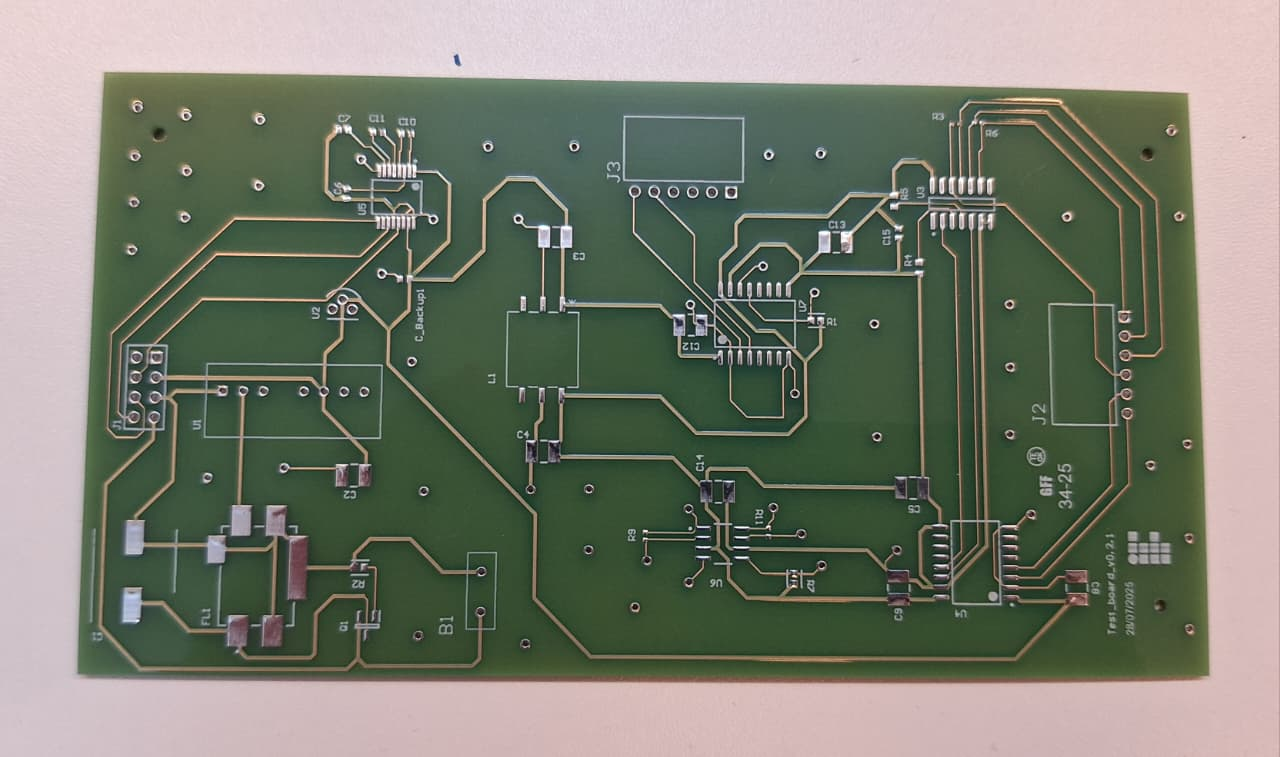
\includegraphics[height=3.8cm]{imagens/III/raw_pcb_1.jpeg}}
        }\hfill
        \subfloat[Vista 3D do protótipo]{
            \frame{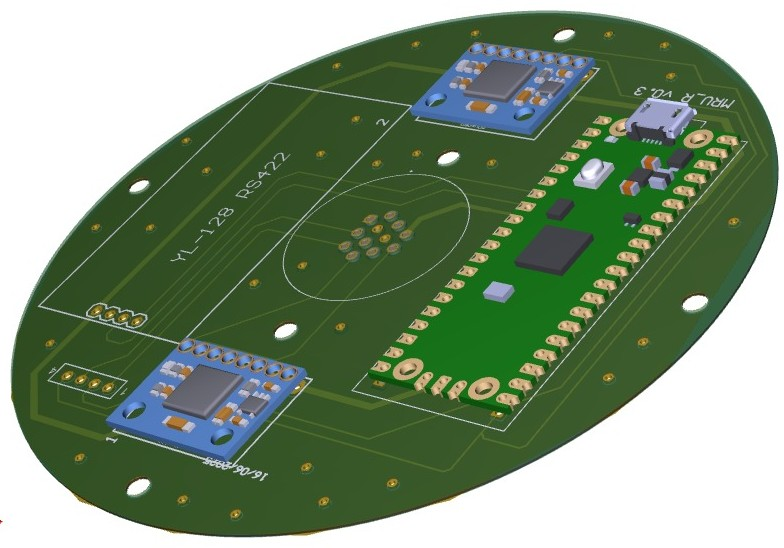
\includegraphics[height=3.8cm]{imagens/II/3d_prot1a.jpeg}}
        }

        \textbf{Fonte:} Autoria Própria
        \label{fig:pcb_v1}
    \end{figure}

    Os testes com a placa de primeira geração validaram o funcionamento dos circuitos de comunicação RS-422 e RS-232, dos reguladores de alimentação e da tecnologia SMD, confirmando que os componentes de montagem superficial são viáveis e reduzem significativamente o volume e o custo de fabricação. A transição para o ESP32-S3 Mini foi decidida com base nos resultados dessa fase.

\subsection{PCB do Primeiro Protótipo (Segunda Geração)}

    Com base nos resultados da placa de teste, foi projetado o primeiro protótipo integrado, substituindo o Raspberry Pi Pico pelo ESP32-S3 Mini (240 MHz, 4 MB flash, 2 MB PSRAM, dimensões de 15,4 $\times$ 20,5 mm). O microcontrolador descrito oferece maior poder de processamento para os algoritmos de fusão, suporte nativo a Bluetooth e Wi-Fi e dimensões reduzidas compatíveis com o encapsulamento cilíndrico.

    \begin{figure}[H]
        \centering
        \caption{Esquemáticos da PCB do Primeiro Protótipo}

        \subfloat[Alimentação e regulação]{
            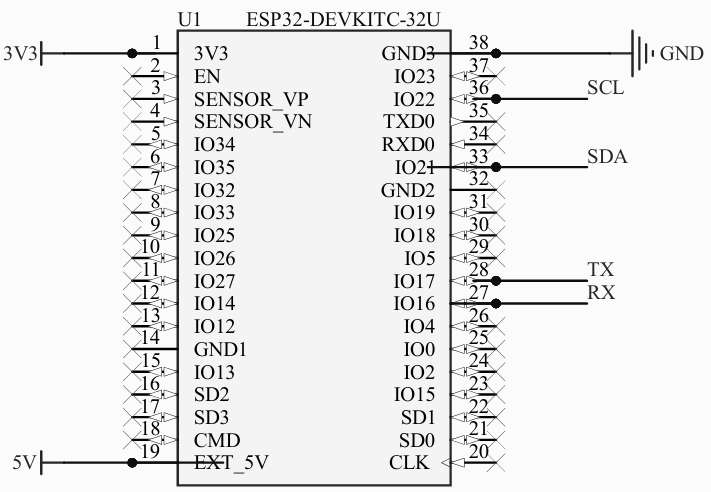
\includegraphics[width=0.4\linewidth]{imagens/II/esq2a.png}
        }\hfill
        \subfloat[Interface RS-422 com KERNEL]{
            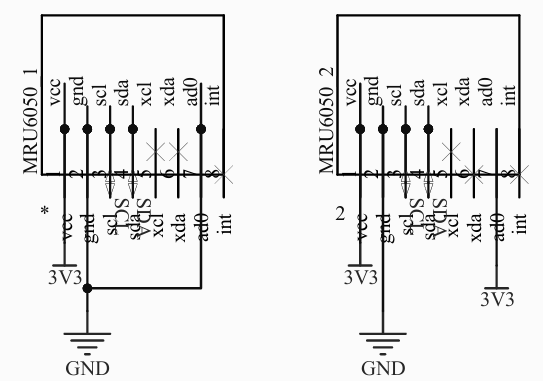
\includegraphics[width=0.4\linewidth]{imagens/II/esq2b.png}
        }

        \subfloat[Interface RS-232 para configuração]{
            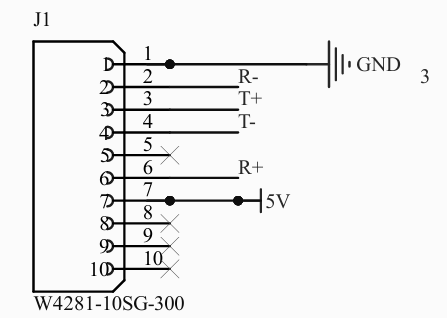
\includegraphics[width=0.4\linewidth]{imagens/II/esq2c.png}
        }\hfill
        \subfloat[Bloco do ESP32-S3 Mini]{
            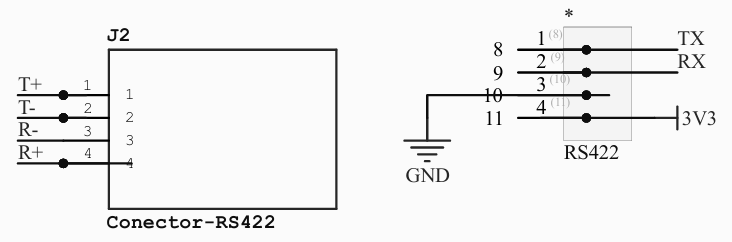
\includegraphics[width=0.4\linewidth]{imagens/II/esq2d.png}
        }

        \textbf{Fonte:} Autoria Própria
        \label{fig:esq2}
    \end{figure}

    Os quatro esquemáticos apresentam os blocos funcionais do sistema embarcado. O bloco de alimentação (superior esquerdo) inclui regulador LDO com filtragem ativa para o sensor KERNEL. O isolamento galvânico da interface RS-422 (superior direito) é garantido por optoacopladores, protegendo o microcontrolador contra surtos de tensão provenientes do barramento industrial.

    \begin{figure}[H]
        \centering
        \caption{PCB do Primeiro Protótipo Montada e Modelo 3D}

        \subfloat[Face Superior]{
            \frame{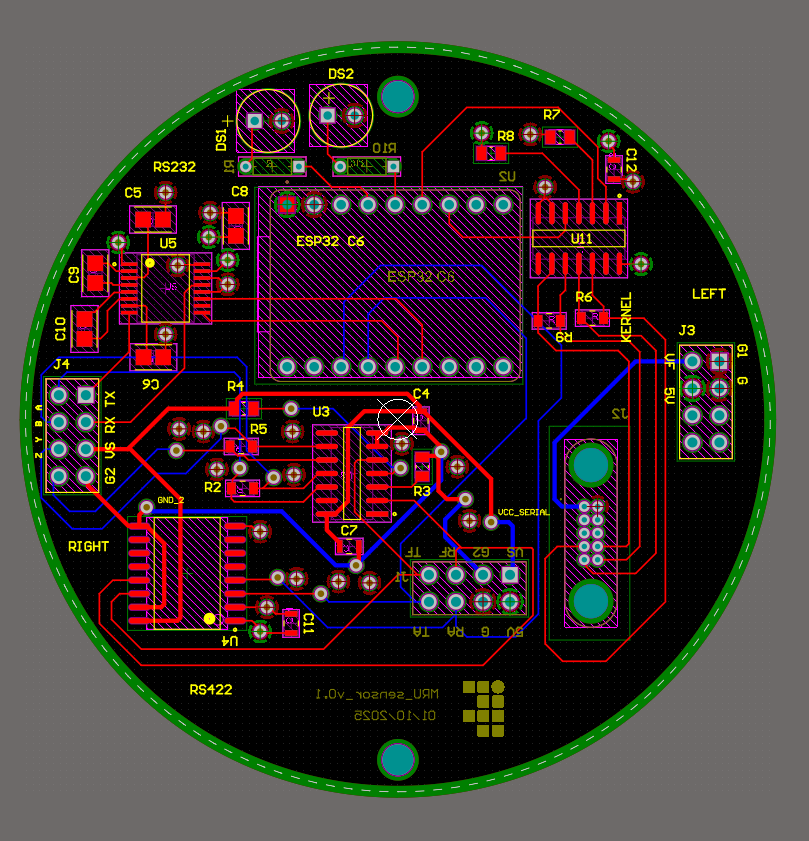
\includegraphics[height=4.5cm]{imagens/III/pcb_atilum_1.png}}
        }\hspace{.4cm}
        \subfloat[Face Inferior]{
            \frame{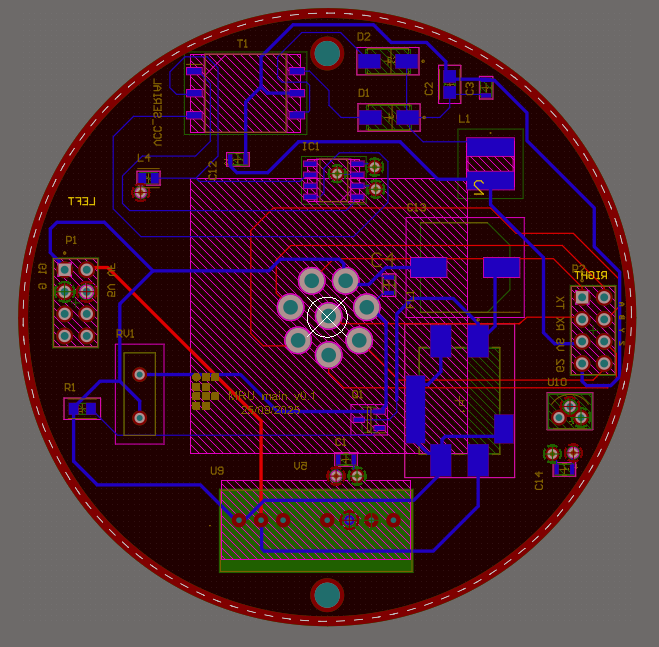
\includegraphics[height=4.5cm]{imagens/III/pcb_atilum_2.png}}
        }\hspace{.4cm}
        \subfloat[Modelo 3D]{
            \frame{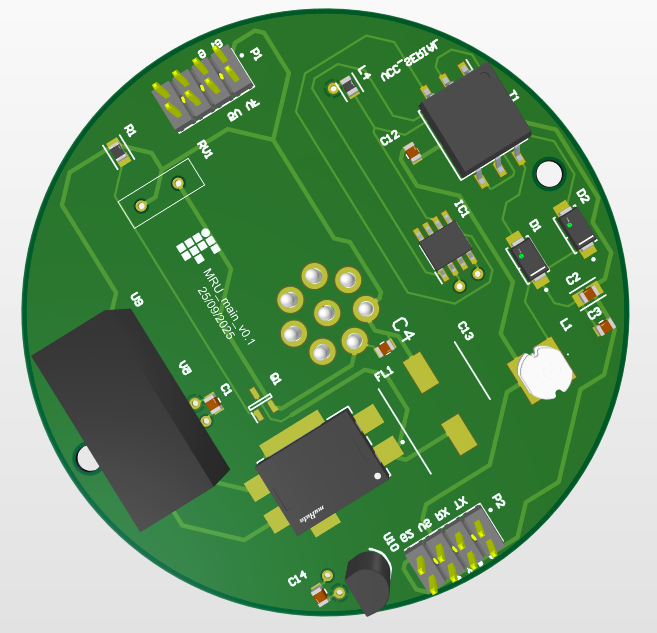
\includegraphics[height=4.5cm]{imagens/III/pcb_3d_1.png}}
        }

        \textbf{Fonte:} Autoria Própria
        \label{fig:pcb_v2}
    \end{figure}

    As faces superior e inferior da placa revelam a distribuição equilibrada dos componentes SMD, com os conectores de alta corrente posicionados na periferia e os blocos de processamento no centro. O modelo 3D confirma a adequação das dimensões ao encapsulamento cilíndrico. Durante os testes de campo com essa placa, foram identificados dois pontos de melhoria: a necessidade de conectar o encoder rotativo diretamente ao ESP32-S3 Mini, e o aprimoramento do circuito RS-232 para maior robustez.

\subsection{PCB Final (Terceira Geração)}

    A placa final incorpora os aprimoramentos identificados nos testes de campo com o primeiro protótipo, incluindo a conexão direta do encoder rotativo ao ESP32-S3 Mini, melhoria no circuito RS-232 e geometria circular para melhor acomodação no compartimento cilíndrico.

    \begin{figure}[!htbp]
        \centering
        \caption{PCB Final e Modelo 3D do Sistema Integrado}

        \subfloat[Placa superior]{
            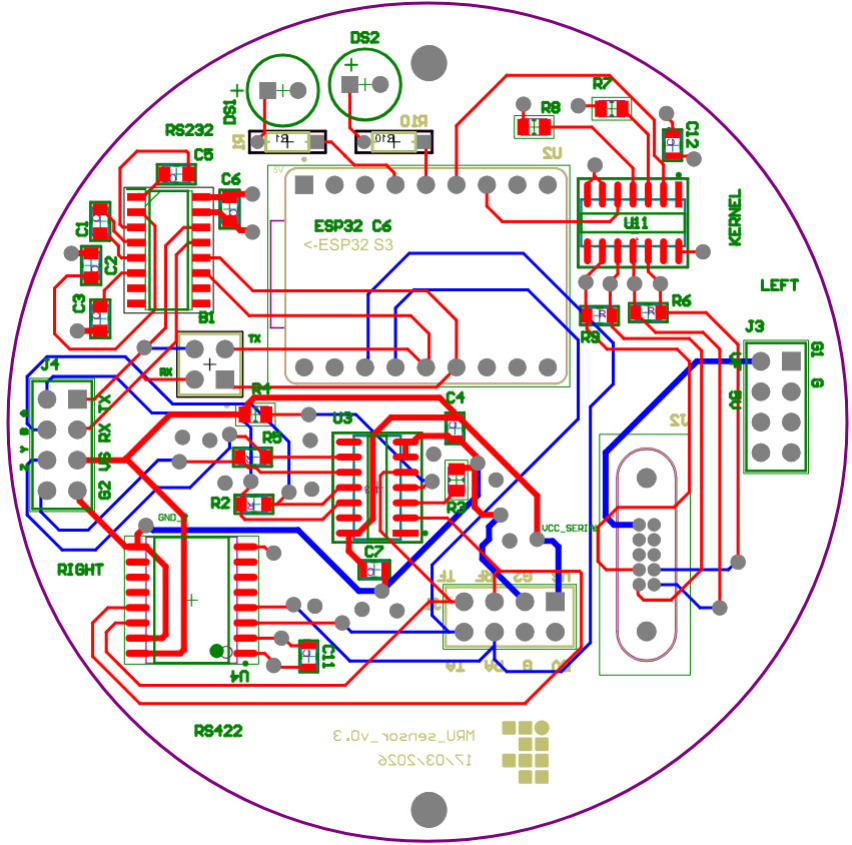
\includegraphics[height=4.5cm]{imagens/V/pcb1.png}
        }\hfill
        \subfloat[Placa inferior]{
            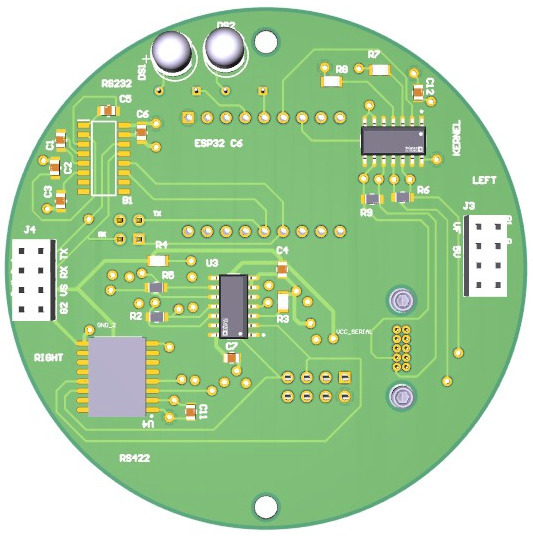
\includegraphics[height=4.5cm]{imagens/V/pcb2.png}
        }\hfill
        \subfloat[Vista 3D integrada]{
            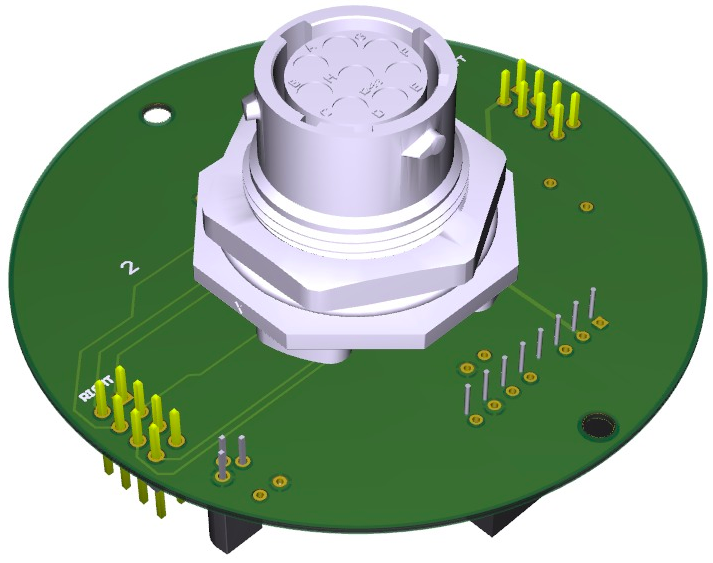
\includegraphics[height=4.5cm]{imagens/V/pcb_3d_1.png}
        }

        \textbf{Fonte:} Autoria Própria
        \label{fig:pcb_final}
    \end{figure}

    A geometria circular da PCB final elimina as quinas que impediam o encaixe no compartimento cilíndrico, reduzindo o diâmetro total da placa de 75 mm para 68 mm. O circuito foi fabricado pela empresa Wego Sistemas utilizando o software Altium Designer, garantindo rastreabilidade de projeto e conformidade com as práticas industriais de produção de PCBs. Com o hardware definitivo estabelecido, as atenções se voltaram para o desenvolvimento do software de comunicação e monitoramento, descrito na próxima seção.


%=============================================================================
\newpage
\section{Software e Protocolo de Comunicação}
%=============================================================================

O DRMM integra três camadas de software, cada uma com funções e interfaces bem delimitadas: o firmware embarcado no ESP32-S3 Mini, o protocolo de comunicação NMEA 0183 e o aplicativo desktop HMS. A clara separação entre essas camadas garante modularidade e facilita a manutenção e atualização independente de cada componente.

\subsection{Firmware Embarcado}

    O firmware foi desenvolvido em C++ utilizando o framework Arduino sobre o ESP32-S3 Mini. Sua arquitetura segue um ciclo de controle em tempo real com três tarefas executadas em ordem fixa por período de amostragem.

    Na primeira tarefa, o ESP32-S3 Mini solicita ao sensor KERNEL os valores de aceleração e velocidade angular via RS-422 a 460800 baud. Na segunda tarefa, os dados recebidos são processados pelos filtros selecionados (Butterworth ou Kalman) e pelo algoritmo de integração de quaternions, resultando nos ângulos de Euler correspondentes. Na terceira tarefa, os ângulos calculados, as acelerações filtradas e a temperatura interna são empacotados em sentenças NMEA 0183 e transmitidos via RS-422 a 38400 baud. Paralelamente, o microcontrolador monitora a porta RS-232 em busca de comandos de configuração.

    A serialização dos dados para comunicação sem fio com o aplicativo HMS utiliza Protocol Buffers (Protobuf), que oferecem representação binária compacta e eficiência de decodificação superior a formatos textuais.

\subsection{Protocolo NMEA 0183 via RS-422}
    O NMEA 0183 é o padrão de comunicação serial adotado pela indústria de navegação marítima, definindo um conjunto de sentenças textuais ASCII transmitidas via RS-422 \cite{marinha2017}. Cada sentença inicia com o caractere \$, contém campos separados por vírgulas e termina com um asterisco seguido por dois caracteres hexadecimais de checksum, calculados pela operação XOR de todos os bytes entre \$ e *. A figura \autoref{fig:protocol_nmea} mostra a organização explicada.

    A sentença emitida pelo DRMM segue o formato abaixo, onde cada campo corresponde a ângulos em graus, acelerações em m/s$^2$, temperatura interna em $^\circ$C e checksum hexadecimal de dois dígitos:

    \begin{center}
    {\small\texttt{\$DRMM,ROLL,PITCH,YAW,AX,AY,AZ,TEMP*XX}}
    \end{center}

     \begin{figure}[H]
        \centering
        \caption{Estrutura da Sentença NMEA 0183 Emitida pelo DRMM}
        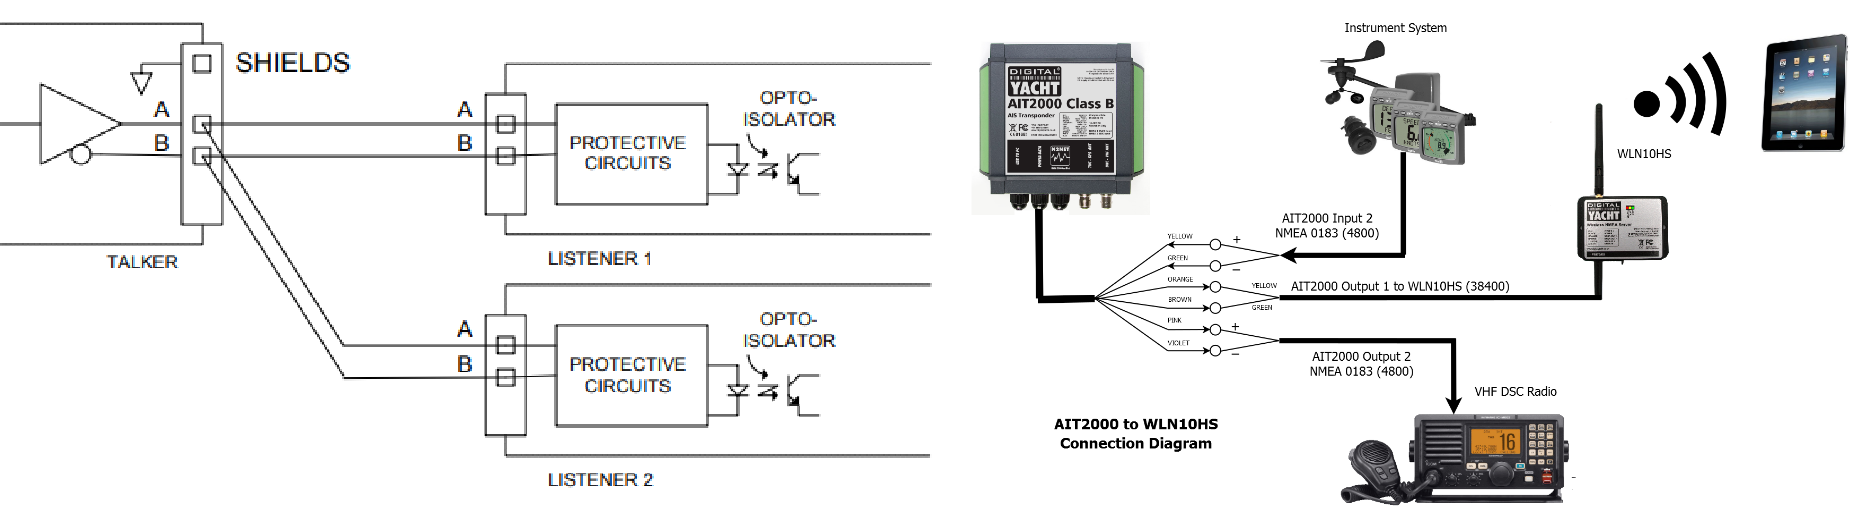
\includegraphics[width=\linewidth]{imagens/III/protocol.png}

        \textbf{Fonte:} Autoria Própria
        \label{fig:protocol_nmea}
    \end{figure}

    Esse formato é compatível com os parsers NMEA utilizados pelos sistemas HMS comerciais, garantindo interoperabilidade imediata. O cálculo do checksum foi implementado em C++ conforme apresentado a seguir.

    \begin{minted}[frame=single, linenos, fontsize=\small]{cpp}
String calcularChecksum(String sentenca) {
    byte checksum = 0;
    for (int i = 1; i < sentenca.length(); i++) {
        if (sentenca[i] == '*') break;
        checksum ^= (byte)sentenca[i];
    }
    String hex = String(checksum, HEX);
    hex.toUpperCase();
    if (hex.length() == 1) hex = "0" + hex;
    return hex;
}
    \end{minted}

\subsection{Protocolo de Configuração via RS-232}

    Para permitir configuração in loco sem necessidade de reprogramação, o DRMM implementa um protocolo proprietário de configuração via RS-232. Os comandos seguem o formato \textbf{\$comando!\{parâmetro\}}, onde os delimitadores \$ e ! identificam início e fim da mensagem, respectivamente. A \autoref{tab:rs232} lista os comandos disponíveis.

    \begin{table}[!htbp]
        \centering
        \caption{Comandos do Protocolo de Configuração RS-232}
        \label{tab:rs232}
        \vspace{-0.2cm}

        \small
        {\renewcommand{\arraystretch}{1.5}
        \begin{longtable}{|m{3.5cm}|m{4cm}|m{6.5cm}|}
        \hline
            \centering\textbf{Comando} & \centering\textbf{Parâmetro} & \centering\textbf{Descrição}\arraybackslash \\
        \hline
            \texttt{\$rate!\{valor\}} & Inteiro (Hz) & Define a frequência de saída de dados \\
        \hline
            \texttt{\$baud!\{valor\}} & 4800 / 9600 / 38400 & Define o baudrate da saída RS-422 \\
        \hline
            \texttt{\$filter!\{tipo\}} & kalman / butterworth & Seleciona o filtro digital ativo \\
        \hline
            \texttt{\$reset!} & --- & Reinicia para configurações padrão \\
        \hline
            \texttt{\$info!} & --- & Retorna versão do firmware e número de série \\
        \hline
        \end{longtable}}

        \small
        \textbf{Fonte:} Autoria Própria
    \end{table}

    O protocolo RS-232 foi projetado para ser simples o suficiente para ser enviado por qualquer terminal serial (Putty, screen, minicom), eliminando a dependência de um software proprietário de configuração. A resposta de confirmação é enviada como sentença NMEA com o campo de status confirmando o comando recebido.

\subsection{Aplicativo HMS (Helideck Monitoring System)}
    O aplicativo HMS foi desenvolvido como software desktop multiplataforma (Windows e Linux) com o framework Tauri, combinando backend em Rust para alto desempenho de comunicação serial e decodificação de sentenças NMEA, e frontend em React com TypeScript para a interface gráfica.

    \begin{figure}[H]
        \centering
        \caption{Aplicativo HMS: Telas de Monitoramento e Banco de Dados}
        \frame{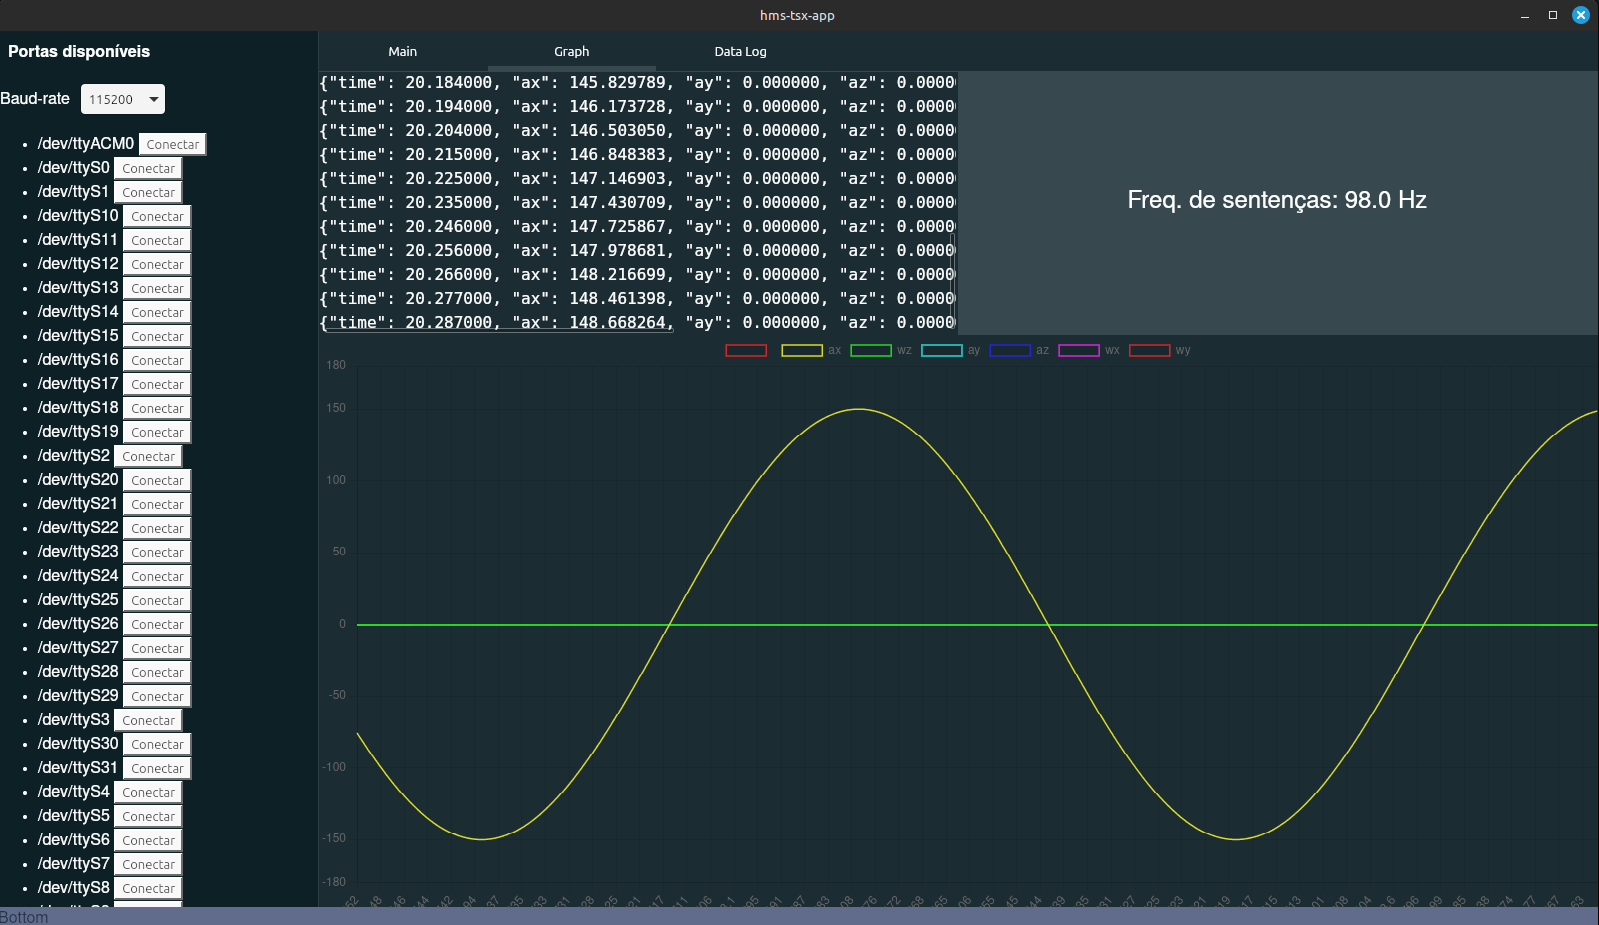
\includegraphics[width=\linewidth]{imagens/III/screenshot_hms_teste.png}}

        \textbf{Fonte:} Autoria Própria
        \label{fig:hms_screens}
    \end{figure}

    A tela de monitoramento em tempo real (esquerda) exibe os gráficos de roll, pitch, yaw e acelerações com atualização a cada ciclo de transmissão em JSON, além de indicadores visuais de alerta quando os ângulos ultrapassam os limites operacionais. A tela de banco de dados (direita) permite consultar e exportar o histórico de medições em formato CSV para análise pós-operação. A \autoref{fig:hms_interface} apresenta o HMS durante uma sessão de teste com o pêndulo de calibração.

    \begin{figure}[!htbp]
        \centering
        \caption{Interface do HMS com Gráficos em Tempo Real durante Teste com Pêndulo}
        \frame{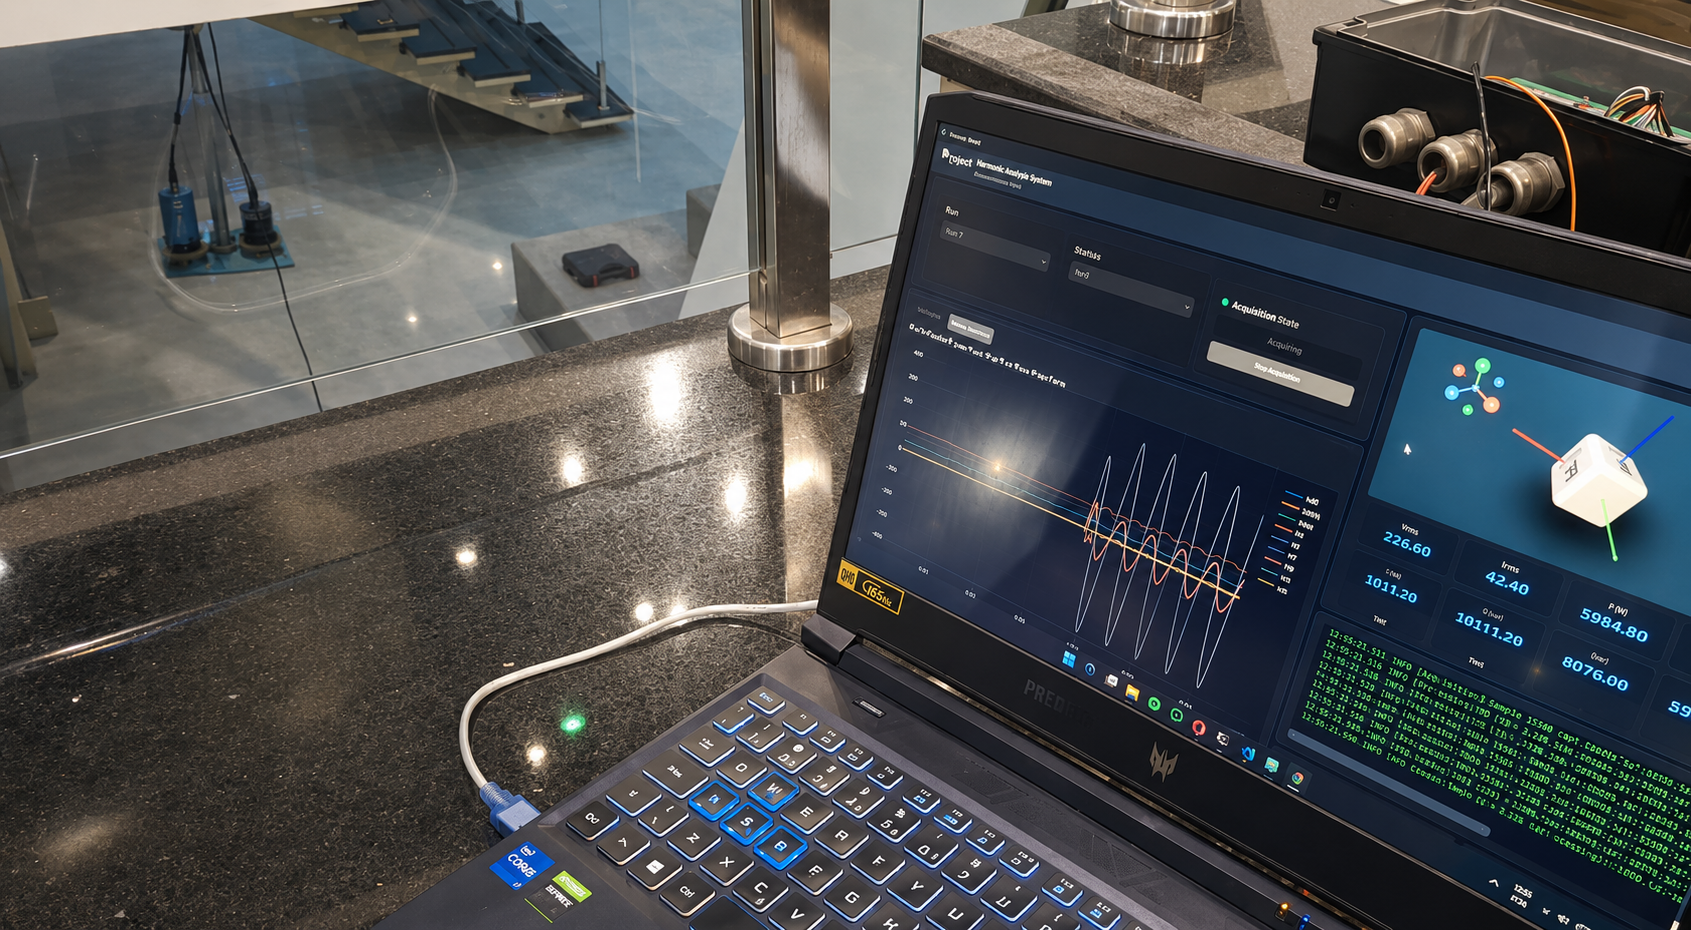
\includegraphics[width=.9\linewidth]{imagens/V/hms_pendulo_teste.png}}

        \textbf{Fonte:} Autoria Própria
        \label{fig:hms_interface}
    \end{figure}

    Na sessão de teste com o pêndulo, os gráficos de roll sobrepõem em tempo real a curva do DRMM (linha azul) e o ângulo de referência calculado a partir dos pulsos do encoder (linha laranja), permitindo verificar visualmente a qualidade da calibração antes de aceitar os coeficientes calculados. Com o software completamente implementado e validado, a atenção foi voltada para o projeto e fabricação do encapsulamento do DRMM, apresentado na próxima seção.

    \subsection{HMS}
        O desenvolvimento do aplicativo desktop de monitoramento foi direcionado para ter um foco comercial e atender às expectativas atuais do setor. As telas do programa foram estruturadas com base em soluções já consolidadas, como o sistema dedicado da empresa Kongsberg. Além disso, o software foi projetado para indicar as variáveis de movimento Pitch, Roll e Yaw de maneira contínua e puramente numérica. Contudo, o foco central dessa abordagem técnica é simplificar a operação diária. Logo, o formato adotado garante aos usuários uma facilidade significativamente maior na visualização dos dados.
        
        \begin{figure}[H]
            \centering
            \caption{HMS Comercial do Sistema}
            \subfloat[Modelo Kongsberg]{
                \frame{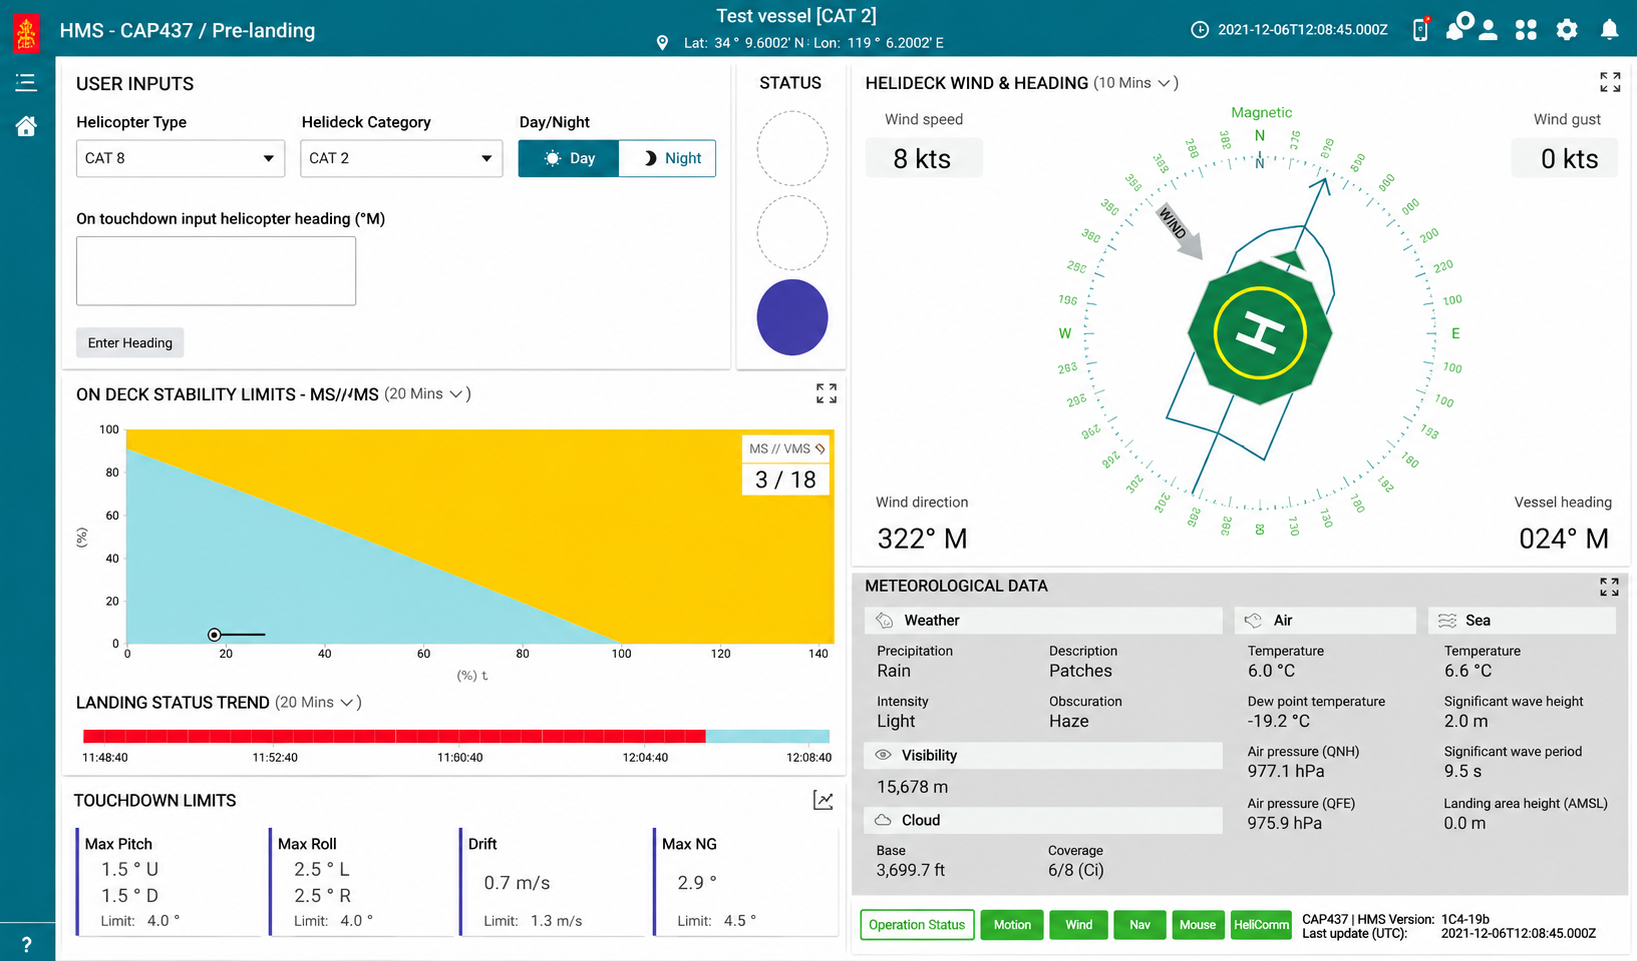
\includegraphics[height=4.6cm]{imagens/V/hms1.png}}
            }\hfill
            \subfloat[Modelo Measure]{
                \frame{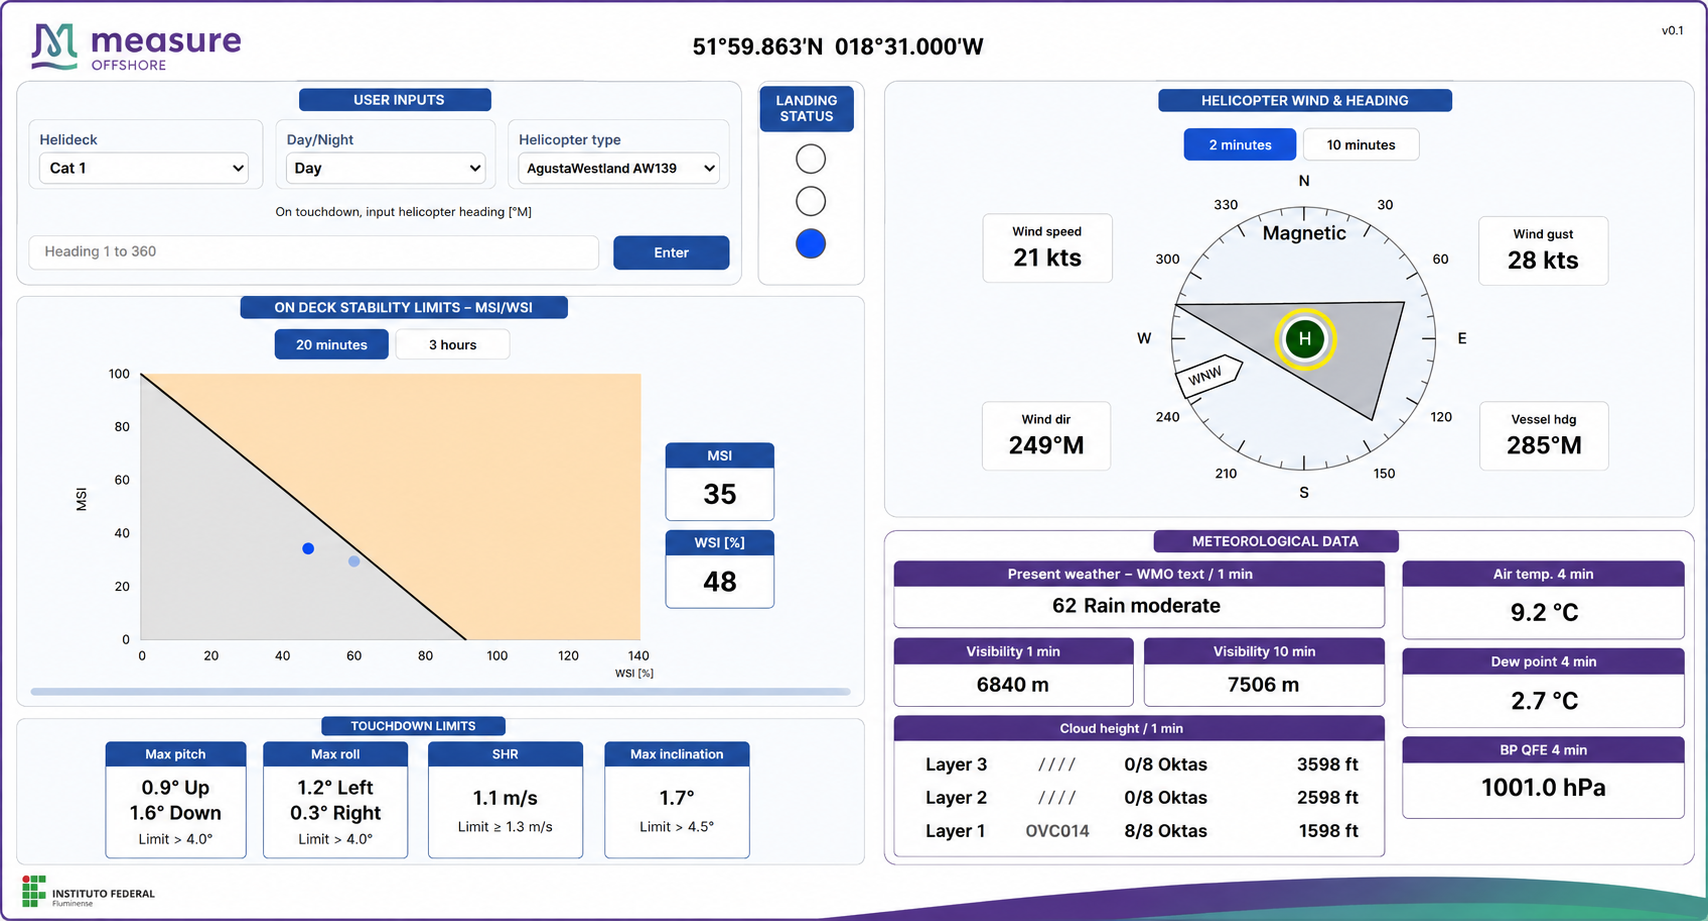
\includegraphics[height=4.6cm]{imagens/V/hms2.png}}
            }

            \textbf{Fonte:} Autoria Própria
            \label{fig:circuito01}
        \end{figure}

        As outras variáveis gráficas e numéricas estão disponíveis no sistema apenas de forma simbólica. Isso ocorre porque somente as três informações de orientação têm origem direta no MRU. Além disso, os demais dados são provenientes de sensores externos que não integram o escopo do projeto atual. Contudo, a aplicação atua como uma ferramenta indicativa totalmente escalável. Logo, o sistema poderá estabelecer comunicação com diversos equipamentos e sensores no futuro, o que permitirá o seu funcionamento integrado em uma estação sensorial embarcada.


%=============================================================================
\newpage
\section{Embalagem e Compartimento}
%=============================================================================

O compartimento do DRMM cumpre duas funções críticas: proteger os componentes eletrônicos do ambiente marítimo (salinidade, umidade, vibração e temperatura) e garantir a rigidez mecânica necessária para que as medições inerciais sejam referenciadas a uma estrutura rígida conhecida. O projeto do compartimento passou por duas gerações.

\subsection{Compartimento em Impressão 3D (Versão Inicial)}

    O compartimento inicial foi projetado em formato cilíndrico com 105 mm de diâmetro e 120 mm de altura, produzido em ABS por impressão 3D. Essa versão permitiu validar o layout interno das placas, a posição dos conectores e o processo de montagem, identificando pontos de melhoria antes da fabricação metálica definitiva.

    \begin{figure}[!htbp]
        \centering
        \caption{Desenhos Técnicos do Compartimento Cilíndrico}

        \subfloat[Tampa Superior]{
            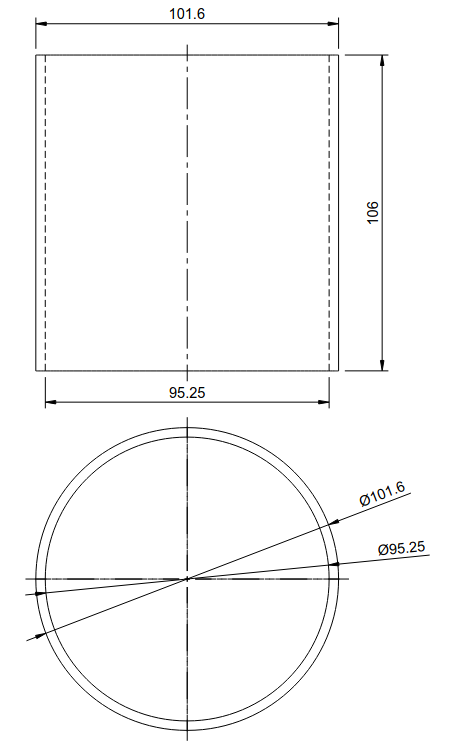
\includegraphics[height=5.5cm]{imagens/III/desenhoA.png}
        }\hfill
        \subfloat[Tampa Inferior]{
            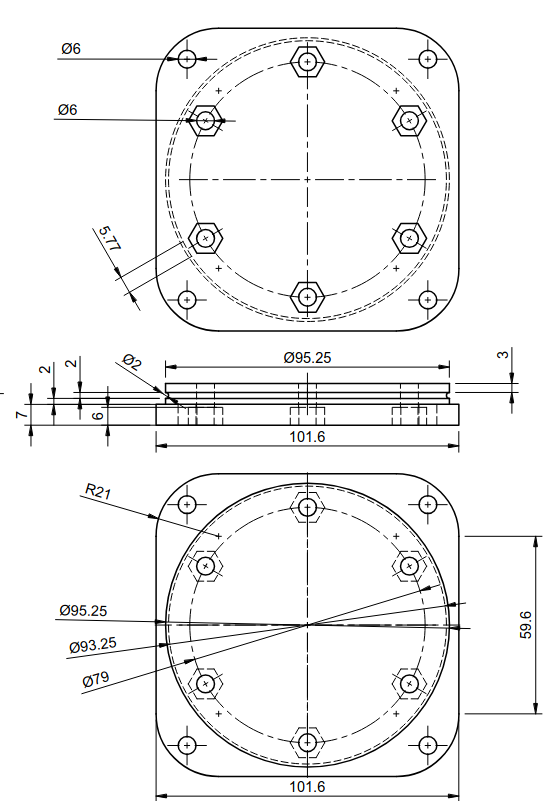
\includegraphics[height=5.5cm]{imagens/III/desenhoB.png}
        }\hfill
        \subfloat[Corpo Cilíndrico]{
            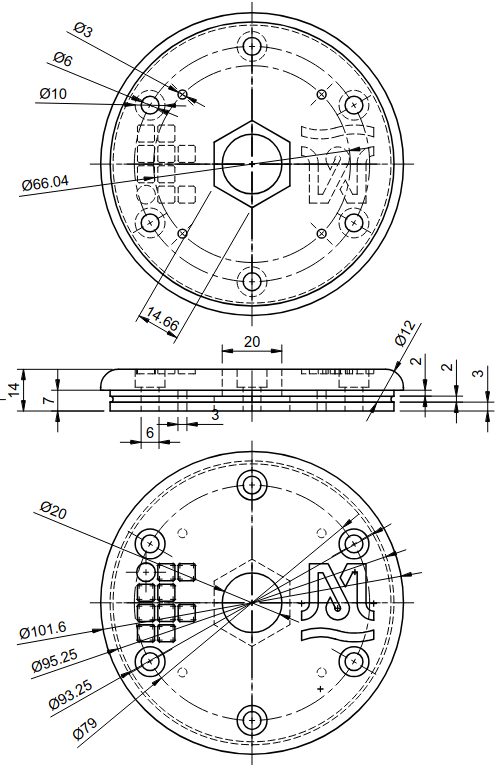
\includegraphics[height=5.5cm]{imagens/III/desenhoC.png}
        }

        \textbf{Fonte:} Autoria Própria
        \label{fig:desenhos_tecn}
    \end{figure}

    Os desenhos técnicos especificam as dimensões nominais das três peças com tolerâncias de $\pm 0{,}1$ mm para as superfícies de vedação. A rosca M4 nas tampas e o ressalto de centragem no corpo cilíndrico garantem o alinhamento das peças durante a montagem, assegurando a compressão uniforme dos anéis O-ring e o nível de proteção IP67.

    \begin{figure}[H]
        \centering
        \caption{Compartimento com as Placas Instaladas}

        \subfloat[Protótipo com Impressão 3D]{
            \frame{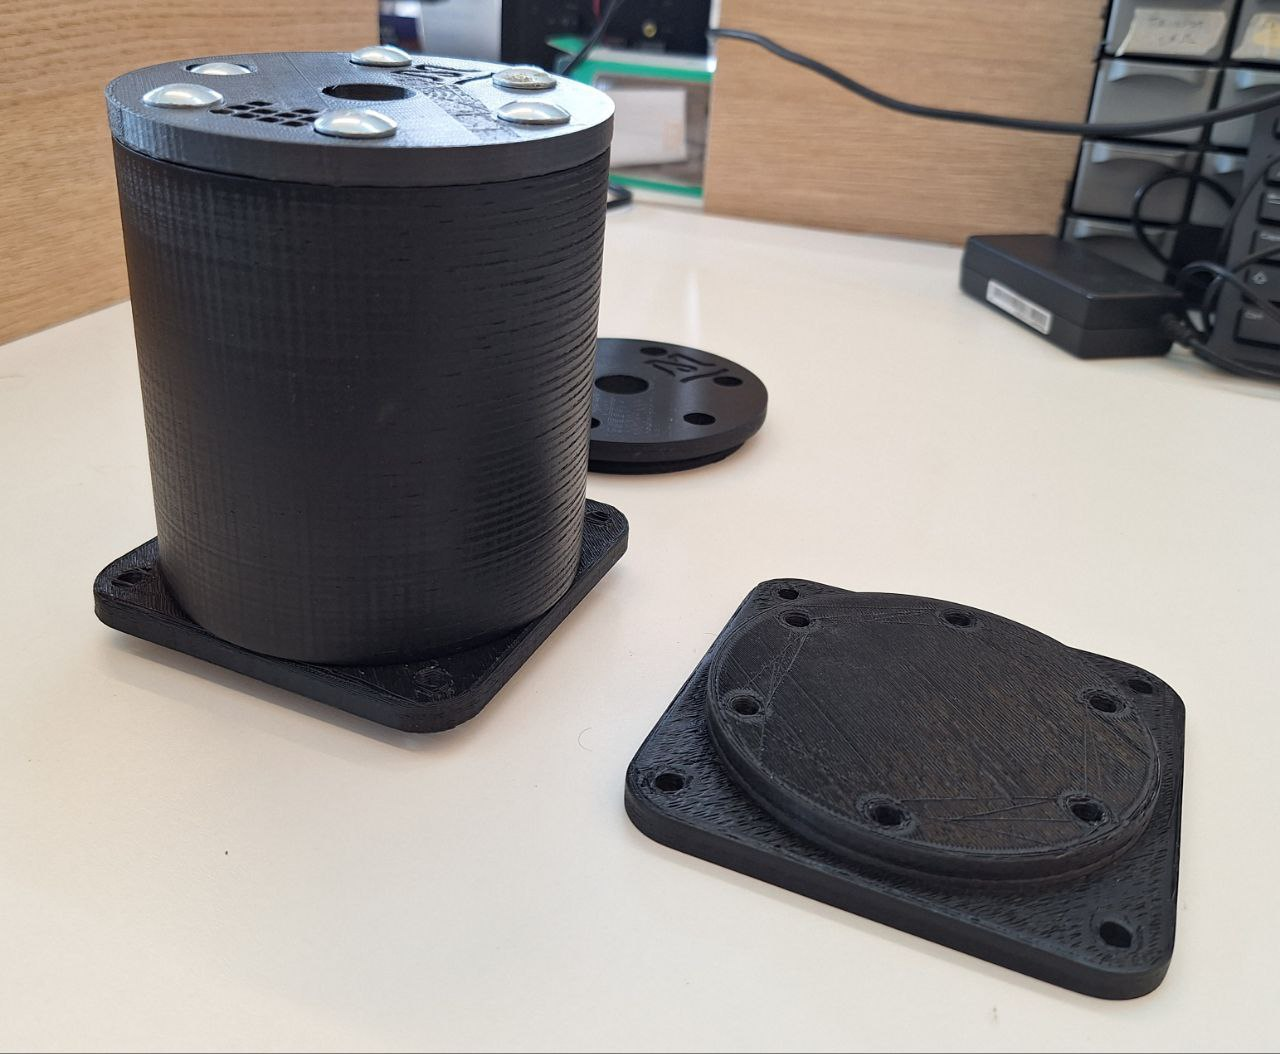
\includegraphics[height=6.5cm]{imagens/III/embalagem01.jpeg}}
        }\hfill
        \subfloat[Embalagem Metálica com Dimensões]{
            \frame{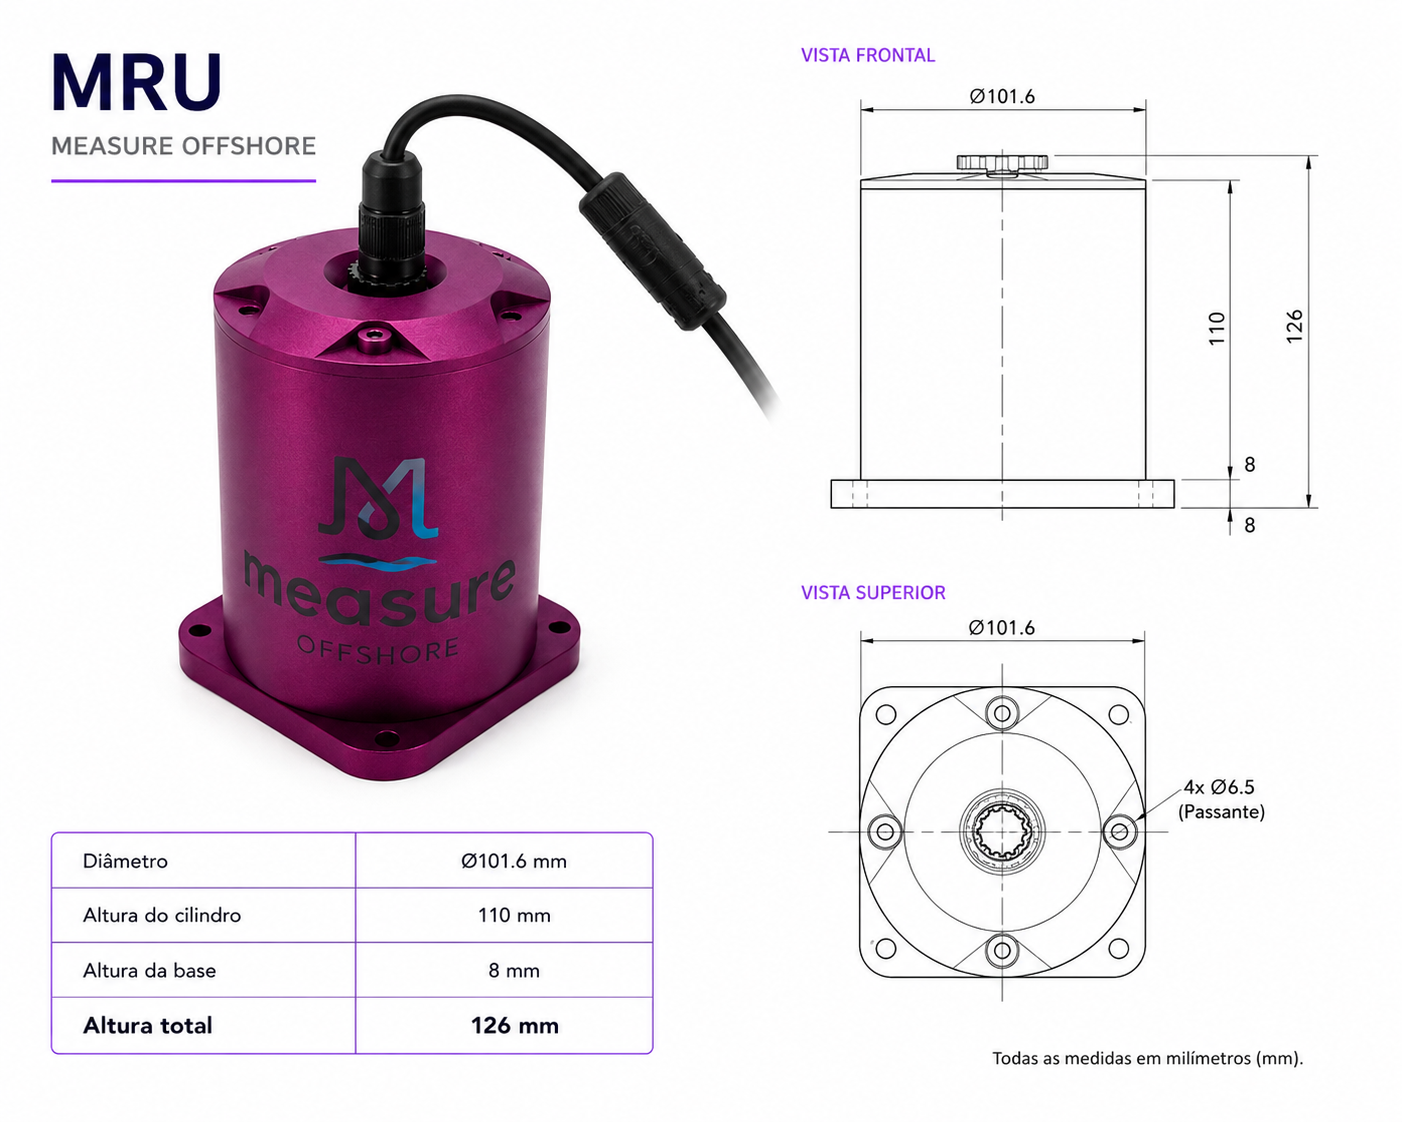
\includegraphics[height=6.5cm]{imagens/V/mru.png}}
        }

        \textbf{Fonte:} Autoria Própria
        \label{fig:emb3d}
    \end{figure}

    A versão em ABS confirmou a viabilidade do layout interno e identificou duas melhorias necessárias: o alargamento do canal de entrada de cabos em 2 mm e o reposicionamento do anel O-ring para uma ranhura mais profunda, garantindo vedação mais eficiente. Esses ajustes foram incorporados ao projeto do compartimento metálico definitivo.

\subsection{Compartimento Metálico Final}

    O compartimento definitivo foi usinado em alumínio liga 6063-T5 com superfície anodizada tipo II, proporcionando proteção IP67, dissipação de calor adequada e resistência mecânica para operação em ambiente offshore.

    \begin{figure}[!htbp]
        \centering
        \caption{Desenho Técnico do Compartimento Metálico Final}
        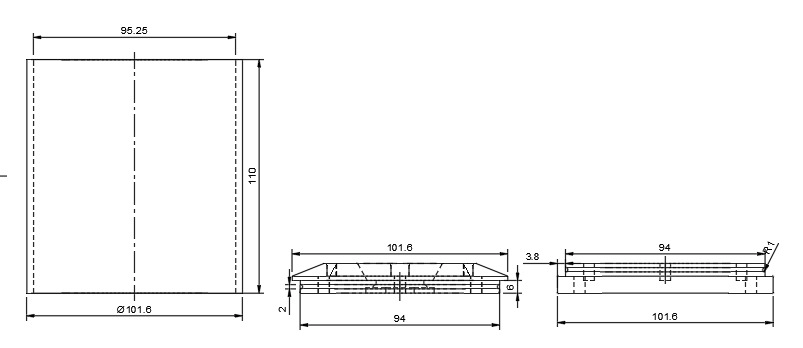
\includegraphics[width=0.9\linewidth]{imagens/V/desenho_tecnico.png}

        \textbf{Fonte:} Autoria Própria
        \label{fig:desenho_tecnico}
    \end{figure}

    O desenho técnico especifica o filete de raio R2 mm nas bordas internas, reduzindo a concentração de tensões mecânicas decorrentes de vibrações e impactos em operação offshore. Os conectores industriais para RS-422 e RS-232 estão instalados na tampa inferior, e a vedação entre as partes é assegurada por anéis O-ring de nitrila resistentes a fluidos salinos.

    \begin{figure}[!htbp]
        \centering
        \caption{Compartimento Metálico do DRMM Usinado}

        \subfloat[Peças prontas para montagem]{
            \frame{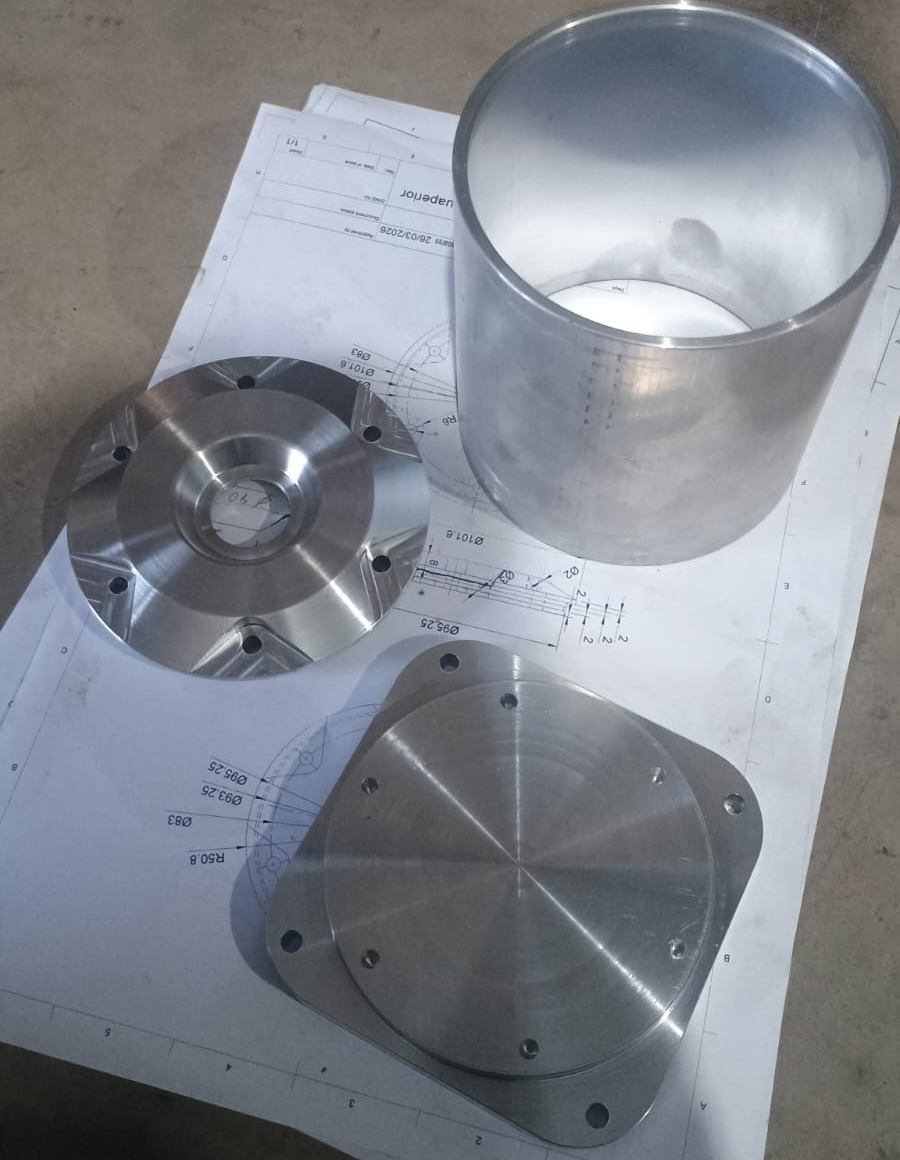
\includegraphics[height=5.5cm]{imagens/V/metal1.png}}
        }\hspace{1cm}
        \subfloat[Montagem final]{
            \frame{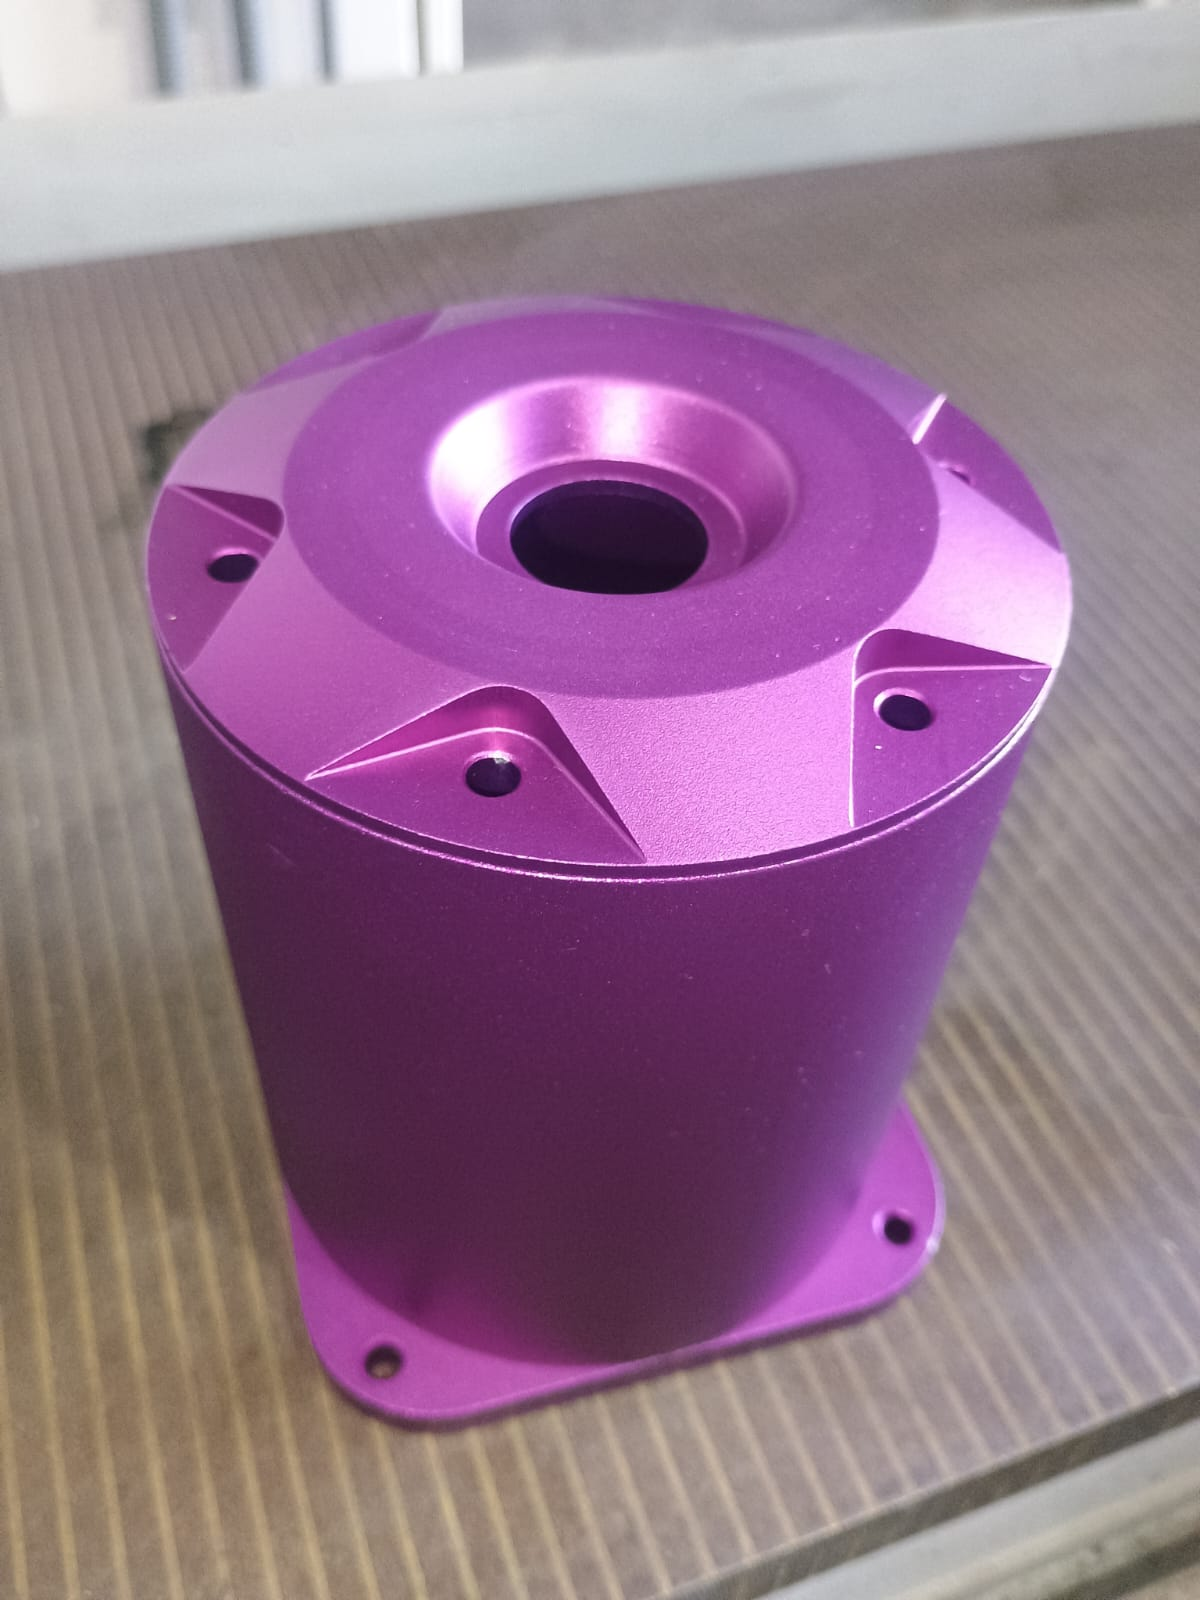
\includegraphics[height=5.5cm]{imagens/V/metal2.png}}
        }

        \textbf{Fonte:} Autoria Própria
        \label{fig:emb_metal}
    \end{figure}

    \begin{figure}[!htbp]
        \centering
        \caption{Vistas do Compartimento Metálico Montado com Sistema Embarcado}

        \subfloat[Vista lateral]{
            \frame{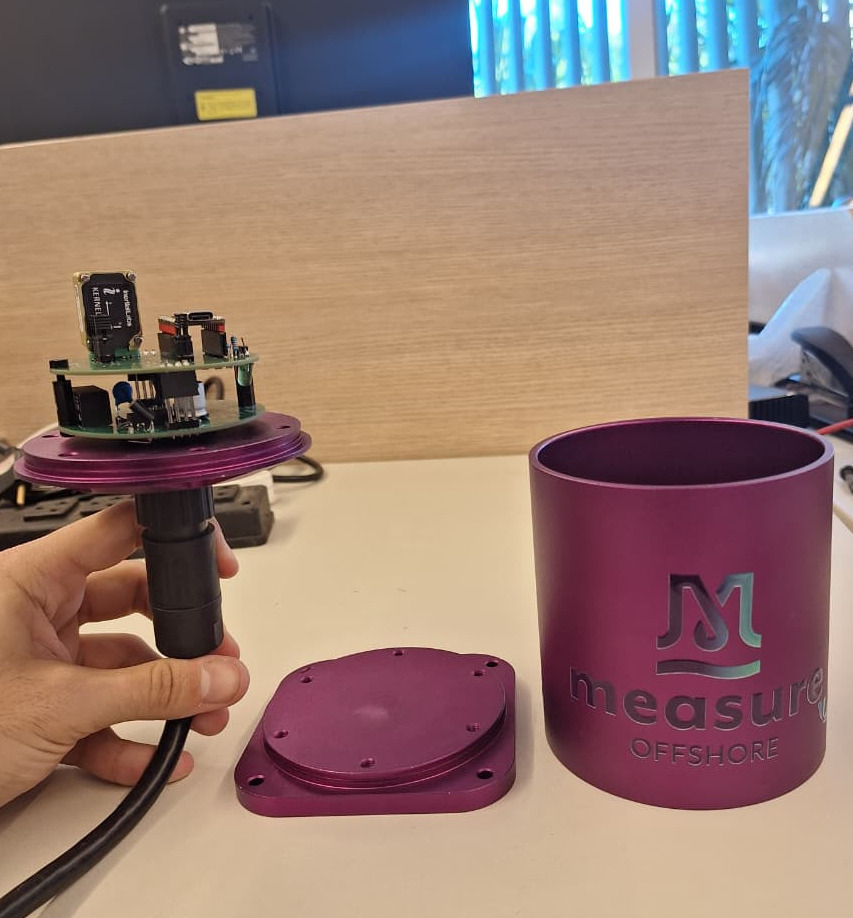
\includegraphics[height=6cm]{imagens/V/embalagem_metal_1.png}}
        }\hfill
        \subfloat[Vista frontal]{
            \frame{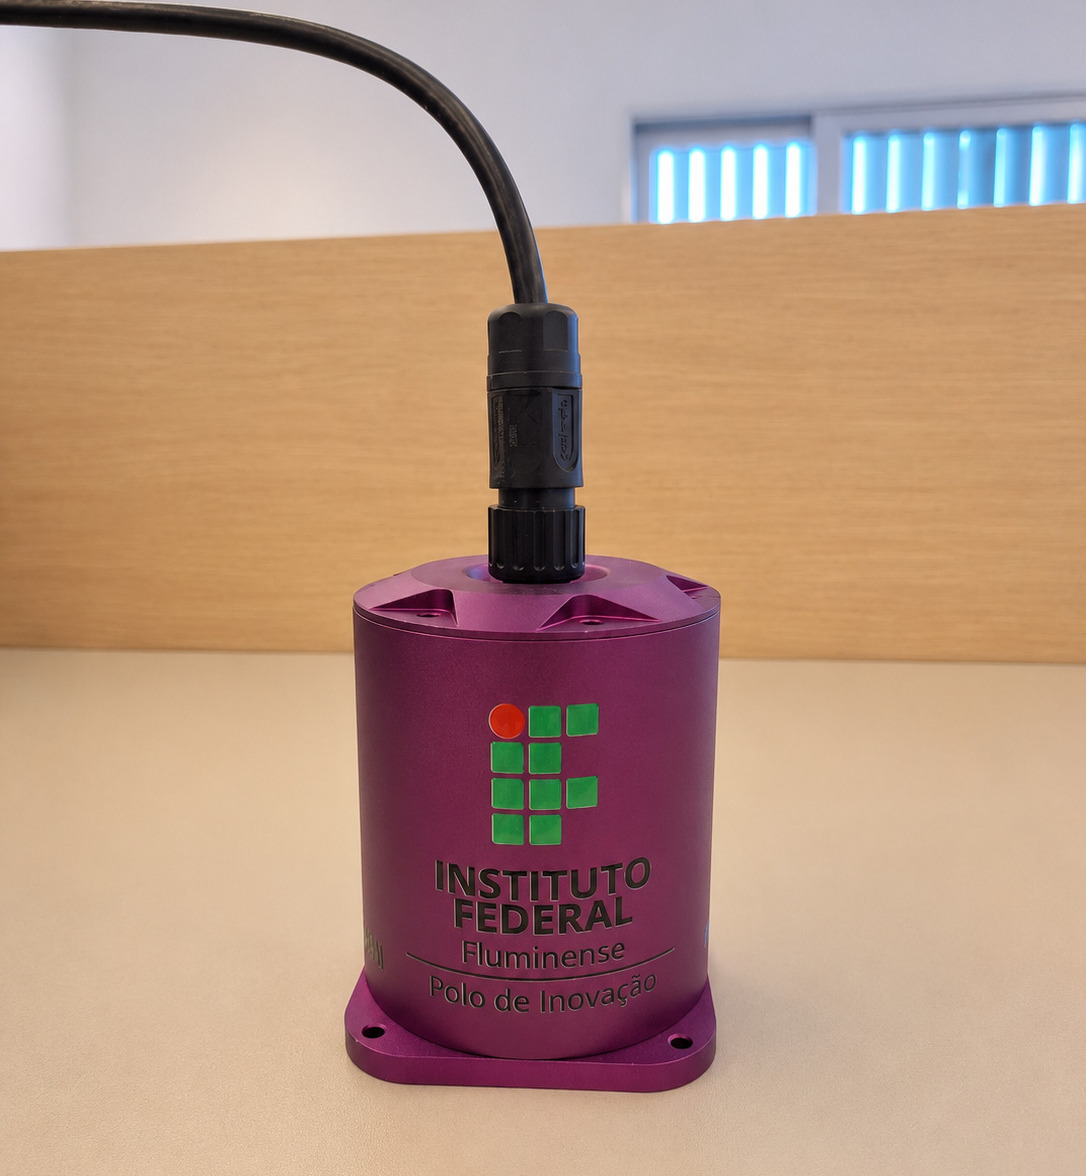
\includegraphics[height=6cm]{imagens/V/embalagem_metal_2.png}}
        }\hfill
        \subfloat[Vista com conectores]{
            \frame{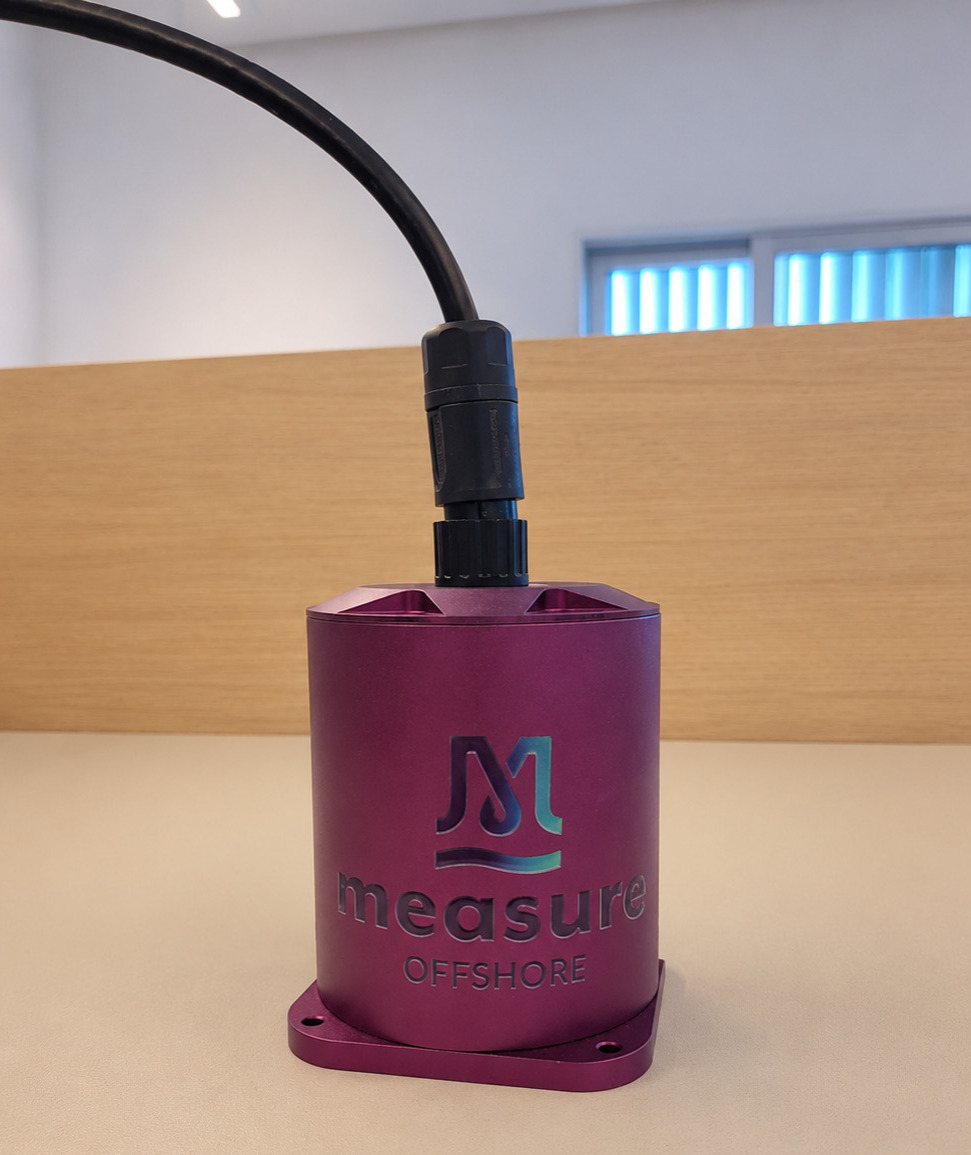
\includegraphics[height=6cm]{imagens/V/embalagem_metal_3.png}}
        }

        \textbf{Fonte:} Autoria Própria
        \label{fig:emb_metal2}
    \end{figure}

    O compartimento usinado apresenta acabamento superficial de alta qualidade, com tolerâncias que garantem o encaixe preciso das tampas no corpo cilíndrico e a compressão uniforme dos anéis O-ring. Os eixos cartesianos X, Y e Z estão gravados na face superior do compartimento para referência de orientação durante a instalação. Com o hardware e o encapsulamento definitivos, a calibração foi o próximo passo, descrita na seção seguinte.


%=============================================================================
\newpage
\section{Calibração e Metodologia Experimental}
%=============================================================================

A calibração de um dispositivo inercial consiste em determinar os coeficientes de correção que minimizam o desvio entre as leituras do sensor e os valores de referência rastreáveis. No DRMM, esse processo envolve testes estáticos (verificação do bias e do ruído em repouso) e testes dinâmicos (verificação da linearidade e da resposta em movimento), utilizando como referência um encoder rotativo de alta precisão montado no eixo de um pêndulo.

\subsection{Estrutura do Pêndulo de Calibração}

    O pêndulo foi montado em uma escada de alumínio com altura de aproximadamente dois metros, utilizando articulação de eixo único que permite oscilações livres no plano de roll com amortecimento mínimo. Como referência angular, adotou-se o encoder incremental modelo E40S6-5000-6-L-5 da Smartec Automação, com resolução de 5000 pulsos por revolução, equivalente a $0{,}072^\circ$ por pulso. Essa resolução é significativamente superior à precisão dinâmica especificada para o KERNEL ($0{,}3^\circ$), garantindo rastreabilidade adequada para a calibração.

    \begin{figure}[!htbp]
        \centering
        \caption{Pêndulo de Calibração e Encoder Incremental}

        \subfloat[Diagrama Esquemático (artigo)]{
            \frame{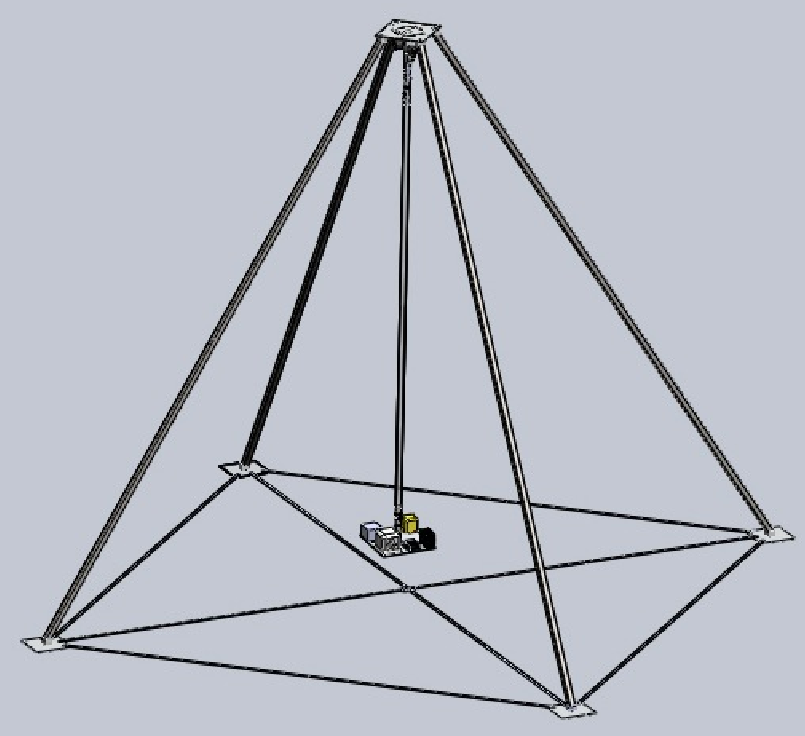
\includegraphics[height=4.5cm]{imagens/V/pendulo2.png}}
        }\hfill
        \subfloat[Encoder E40S6-5000-6-L-5]{
            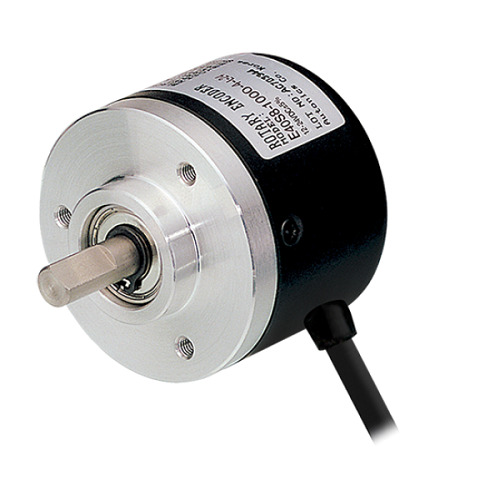
\includegraphics[height=4.5cm]{imagens/V/encoder1.png}
        }\hfill
        \subfloat[Encoder instalado no eixo do pêndulo]{
            \frame{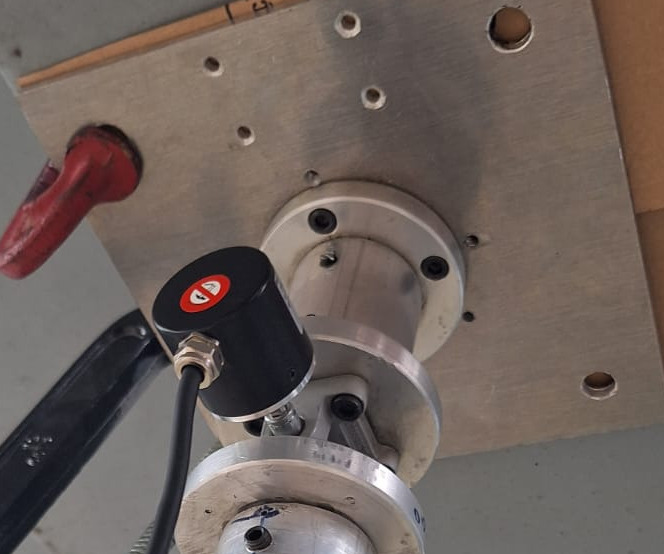
\includegraphics[height=4.5cm]{imagens/V/encoder2.png}}
        }

        \textbf{Fonte:} Autoria Própria
        \label{fig:pendulo}
    \end{figure}

    A arquitetura do pêndulo simples é vantajosa pois o movimento segue uma função senoidal com amortecimento exponencial natural do atrito do ar, dispensando motores ou atuadores artificiais. Isso permite que os testes dinâmicos e estáticos sejam realizados sequencialmente em uma única sessão: primeiro as oscilações de grande amplitude (calibração dinâmica) e, na sequência, o pêndulo para naturalmente (calibração estática), sem intervenção do operador.

\subsection{Protocolo de Calibração}

    O protocolo de calibração foi definido com base em procedimentos similares aos adotados pela Kongsberg Maritime \cite{kongsberg2024}. Cada sessão compreende: aquecimento de 5 minutos em movimento lento (estabilização térmica e convergência de bias), fase dinâmica de 20 minutos com oscilações entre $\pm 2^\circ$ e $\pm 15^\circ$, fase estática de 10 minutos em repouso e processamento dos dados pelo HMS para geração dos coeficientes de calibração por regressão linear.

    \begin{figure}[H]
        \centering
        \caption{Validação do Encoder e Diagrama de Calibração}
        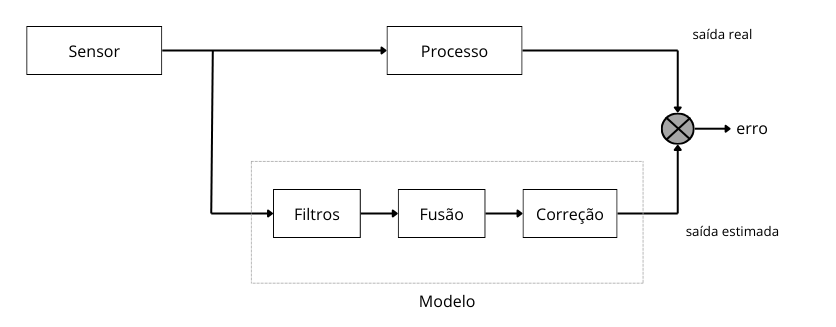
\includegraphics[height=7cm]{imagens/IV/diagrama.png}

        \textbf{Fonte:} Autoria Própria
        \label{fig:calib_proto}
    \end{figure}

    O teste de repetibilidade do encoder (esquerda) confirma que a leitura de posição é consistente entre ciclos de movimento, com desvio máximo de 1 pulso ($0{,}072^\circ$) para a mesma posição angular. O diagrama de fluxo (direita) apresenta as etapas da calibração de forma sequencial, garantindo que as condições de aquecimento e estabilização sejam sempre respeitadas antes da coleta dos dados de referência.

\subsection{Testes no Laboratório LAMCE}

    Os experimentos de calibração foram realizados no Laboratório de Análises e Manutenção de Componentes Eletrônicos (LAMCE), onde temperatura e interferências eletromagnéticas foram controladas para assegurar condições reprodutíveis.

    \begin{figure}[!htbp]
        \centering
        \caption{Testes de Calibração no LAMCE}

        \subfloat[DRMM e MRU montados no pêndulo]{
            \frame{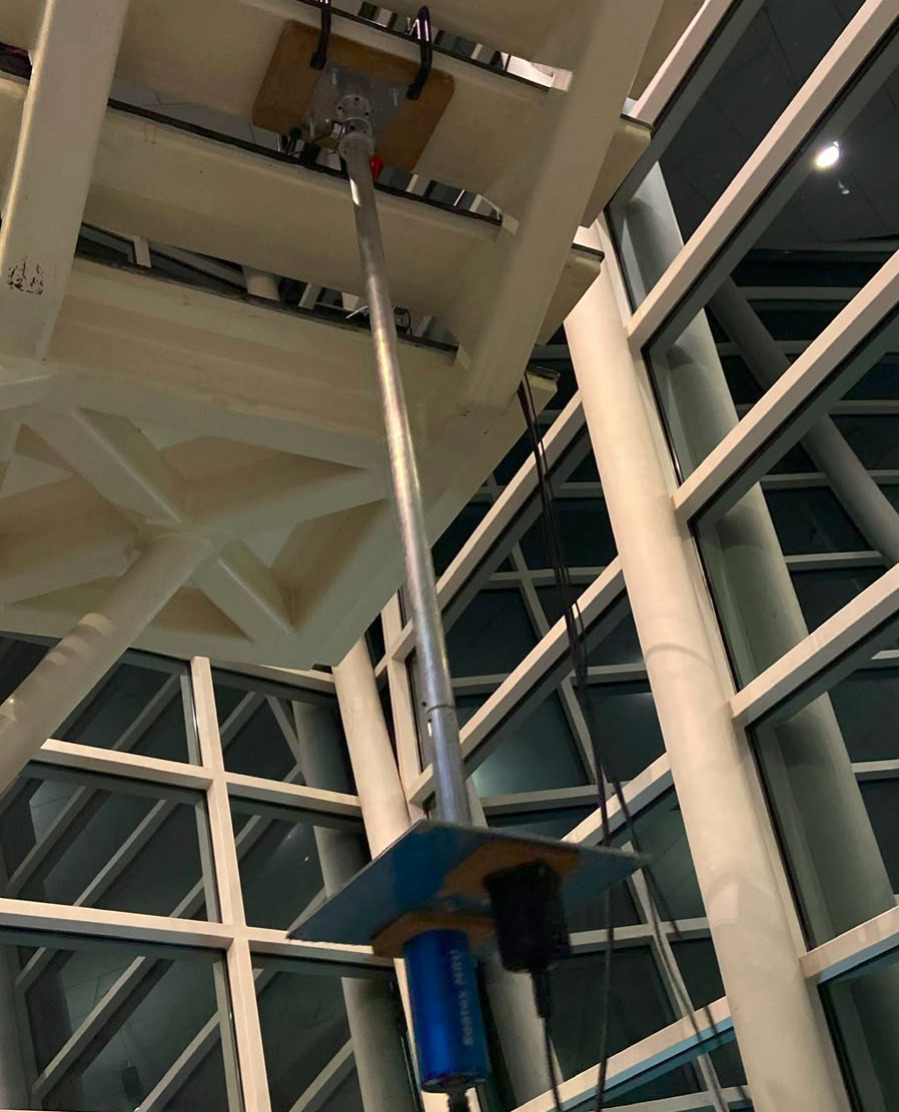
\includegraphics[height=10cm]{imagens/V/pendulo_lamce.png}}
        }\hspace{0.5cm}
        \subfloat[Vista geral do laboratório]{
            \frame{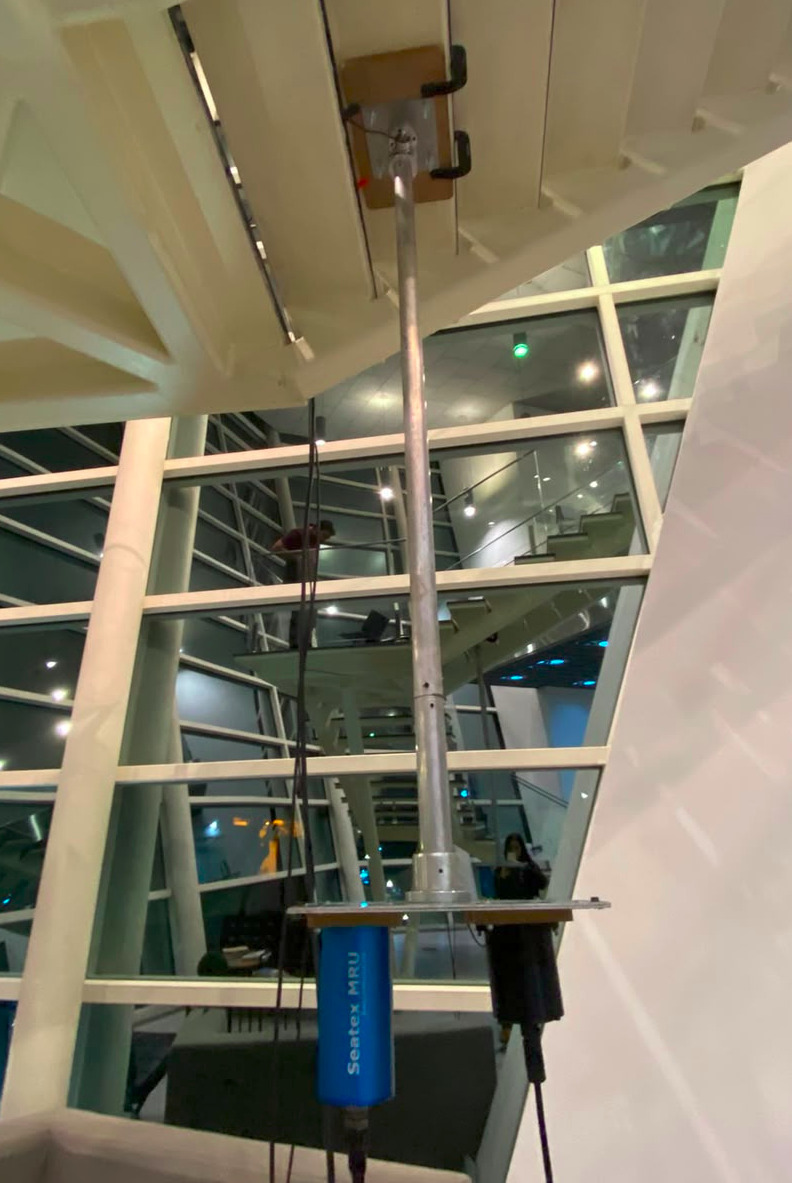
\includegraphics[height=10cm]{imagens/V/pendulo_lamce2.png}}
        }

        \textbf{Fonte:} Autoria Própria
        \label{fig:lamce}
    \end{figure}

    O painel esquerdo mostra o DRMM e o Kongsberg MRU 5 fixados lado a lado na plataforma do pêndulo, na mesma orientação e sob as mesmas condições de temperatura e vibração. Essa disposição paralela é fundamental para garantir que qualquer diferença entre as medições dos dois dispositivos seja atribuída exclusivamente à diferença de desempenho, e não a condições ambientais distintas. Os resultados obtidos nesses experimentos são analisados na seção seguinte.


%=============================================================================
\newpage
\section{Resultados e Análise Comparativa}
%=============================================================================

\subsection{Resultado da Calibração}

    A \autoref{fig:calib_result} apresenta a curva de correlação entre os ângulos medidos pelo DRMM e os ângulos de referência fornecidos pelo encoder rotativo ao longo de um ciclo completo de oscilações do pêndulo.

    \begin{figure}[!htbp]
        \centering
        \caption{Curva de Correlação entre DRMM e Encoder Rotativo}
        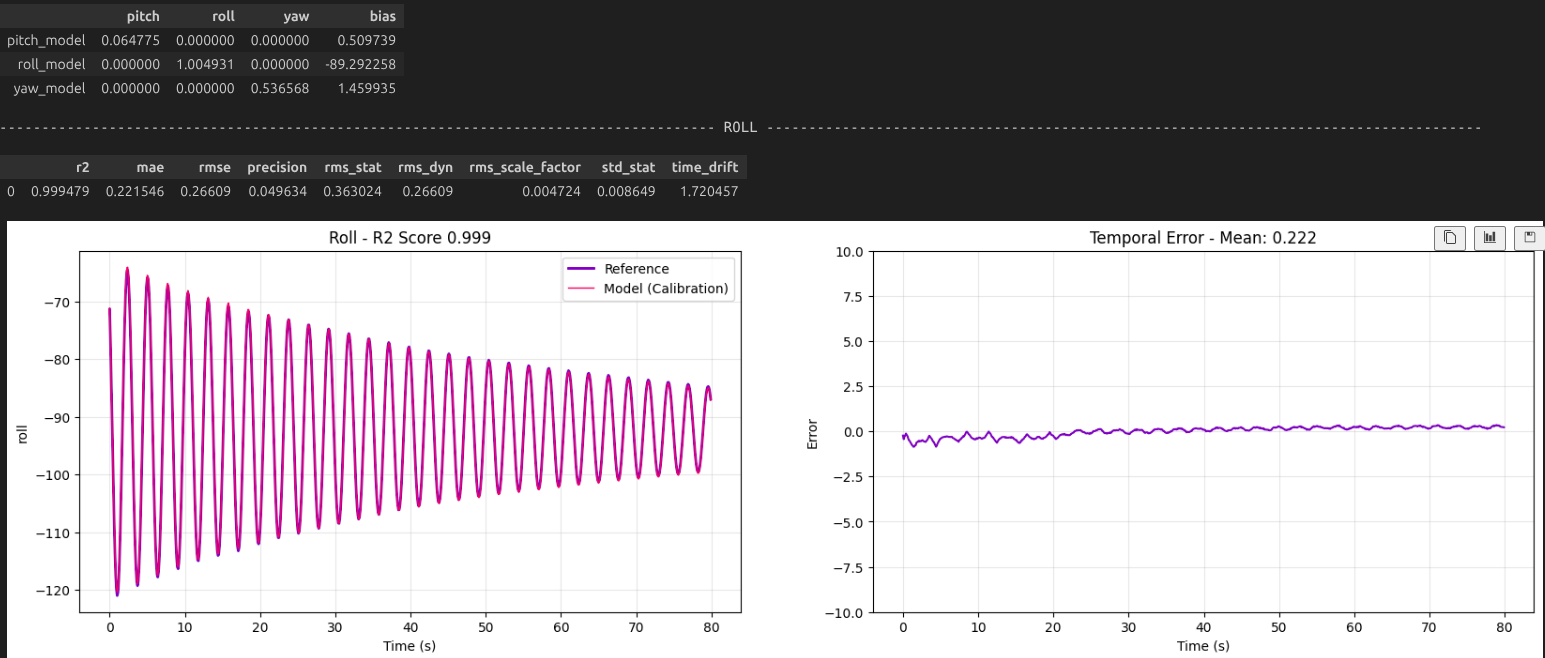
\includegraphics[width=0.82\linewidth]{imagens/V/calib01.png}

        \textbf{Fonte:} Autoria Própria
        \label{fig:calib_result}
    \end{figure}

    O ajuste linear resultou em coeficiente de determinação $R^2 = 0{,}9995$, indicando que 99,95\% da variância das medições do DRMM é explicada pelo modelo linear de calibração. A dispersão dos pontos ao redor da linha de ajuste é mínima, com raiz quadrada do erro médio quadrático (RMSE) inferior a 0,05$^\circ$, dentro da especificação de precisão estática do sensor. A linearidade confirmada permite que um único coeficiente angular e um intercepto sejam suficientes para corrigir todo o range de medição do dispositivo.

    \begin{figure}[!htbp]
        \centering
        \caption{Sobreposição Temporal das Curvas de DRMM e Referência}

        \subfloat[Ciclo completo]{
            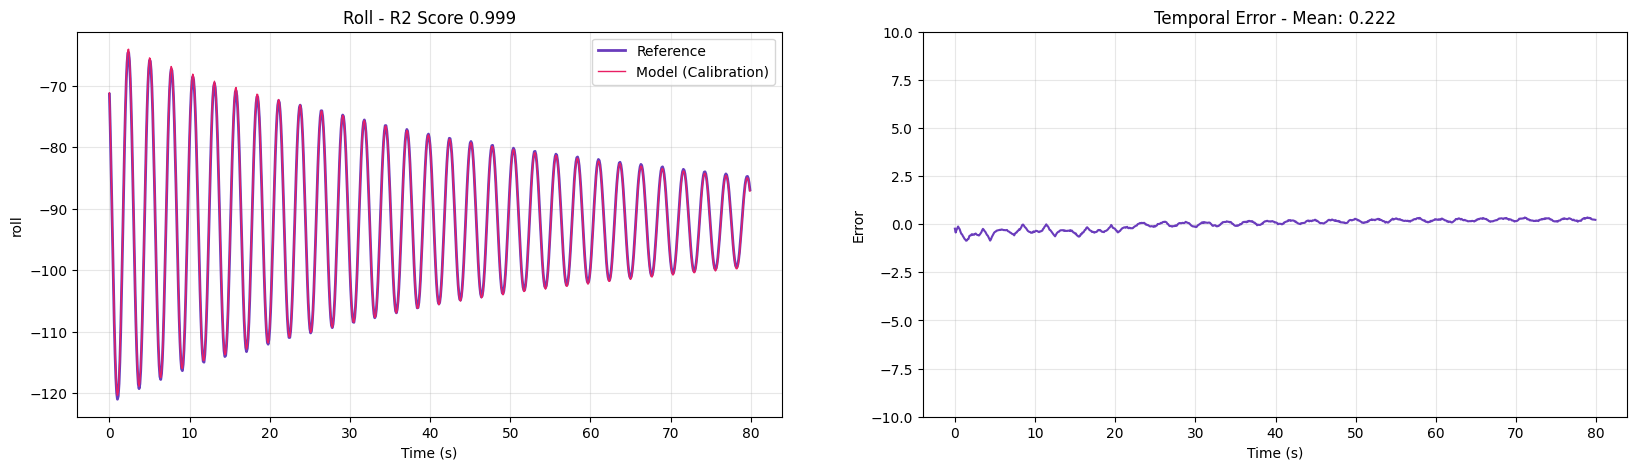
\includegraphics[width=0.47\linewidth]{imagens/V/comparacao1.png}
        }\hfill
        \subfloat[Detalhe na região de pico]{
            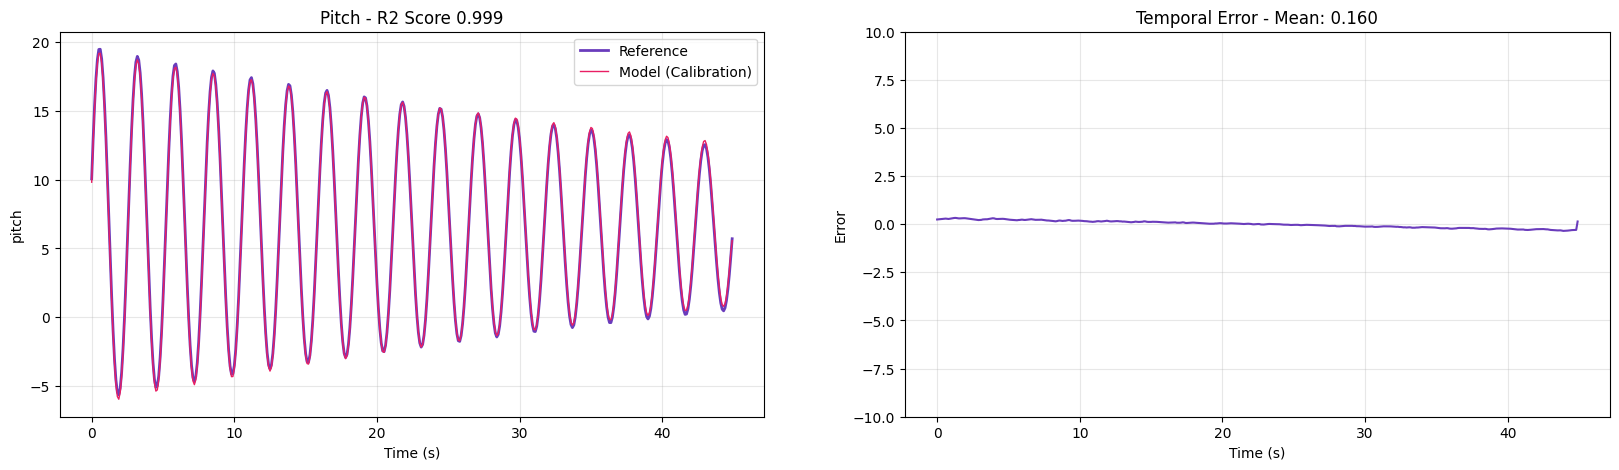
\includegraphics[width=0.47\linewidth]{imagens/V/comparacao02.png}
        }

        \textbf{Fonte:} Autoria Própria
        \label{fig:comparacao_calib}
    \end{figure}

    A sobreposição temporal (Figura~\ref{fig:comparacao_calib}) confirma que o DRMM acompanha com fidelidade a curva do encoder, incluindo nos pontos de máxima amplitude, onde a velocidade angular é maior e os erros de integração tendem a ser mais pronunciados. O detalhe na região de pico (direita) evidencia que o atraso de fase entre as duas curvas é inferior a um período de amostragem (5 ms a 200 Hz), resultado compatível com o tempo de resposta especificado para o filtro de Kalman implementado.

\subsection{Análise Comparativa com MRUs Comerciais}
    A \autoref{tab:comparacao_mercado} compara as especificações técnicas do DRMM com os dois principais MRUs comerciais utilizados pelo setor offshore.

    \begin{table}[H]
        \centering
        \caption{Comparação do DRMM com MRUs Comerciais de Referência}
        \label{tab:comparacao_mercado}
        \vspace{-0.2cm}

        \small
        {\renewcommand{\arraystretch}{1.5}
        \begin{longtable}{|c|c|c|c|}
        \hline
            \fcol{0.22}{\textbf{Especificação}} &
            \col{0.24}{\textbf{DRMM (este projeto)}} &
            \col{0.24}{\textbf{Kongsberg MRU 5}} &
            \col{0.24}{\textbf{KERNEL-120}} \\
        \hline
            \fcol{0.22}{Precisão estática Roll e Pitch} &
            \col{0.24}{$\leq 0{,}03^\circ$ RMS} &
            \col{0.24}{0,03$^\circ$ RMS} &
            \col{0.24}{0,02$^\circ$ RMS} \\
        \hline
            \fcol{0.22}{Precisão dinâmica} &
            \col{0.24}{$\leq 0{,}10^\circ$ RMS} &
            \col{0.24}{0,05$^\circ$ RMS} &
            \col{0.24}{0,03$^\circ$ RMS} \\
        \hline
            \fcol{0.22}{Interface de saída} &
            \col{0.24}{NMEA 0183, RS-422} &
            \col{0.24}{NMEA 0183, RS-422} &
            \col{0.24}{RS-422 (2 Mbit/s)} \\
        \hline
            \fcol{0.22}{Proteção IP} &
            \col{0.24}{IP67} &
            \col{0.24}{IP67} &
            \col{0.24}{IP67} \\
        \hline
            \fcol{0.22}{Fabricação} &
            \col{0.24}{Nacional (Brasil)} &
            \col{0.24}{Noruega} &
            \col{0.24}{EUA} \\
        \hline
        \end{longtable}}

        \small
        \textbf{Fonte:} Autoria Própria com base em \cite{kongsberg2006, inertiallabs2021}
    \end{table}

    O DRMM atingiu precisão estática equivalente ao Kongsberg MRU 5 (0,03$^\circ$ RMS), com interface de comunicação idêntica (NMEA 0183 via RS-422), proteção IP67 e fabricação nacional. A precisão dinâmica do DRMM ($\leq 0{,}10^\circ$ RMS), embora acima da do Kongsberg MRU 5 (0,05$^\circ$ RMS), atende às faixas de alerta definidas pela NORMAM-27/DPC para operações em helidecks offshore, configurando o dispositivo como tecnicamente apto para a aplicação.

    \begin{figure}[!htbp]
        \centering
        \caption{Comparação entre Leituras do DRMM e do Kongsberg MRU em Teste de Campo}

        \subfloat[Eixo de roll]{
            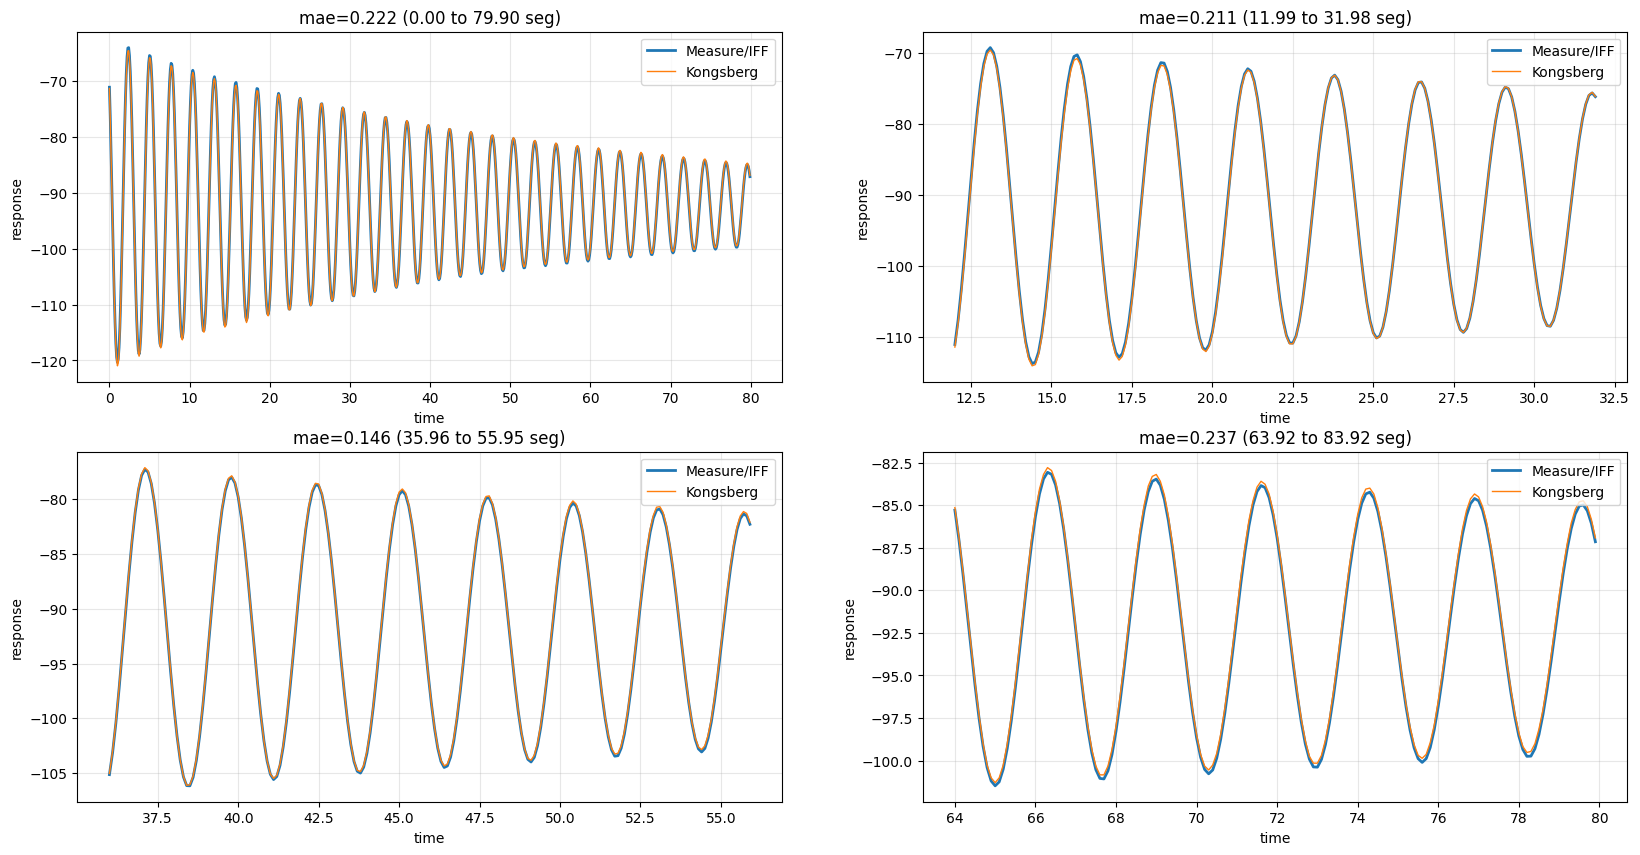
\includegraphics[width=0.47\linewidth]{imagens/V/comp0.png}
        }\hfill
        \subfloat[Resposta em frequência comparada]{
            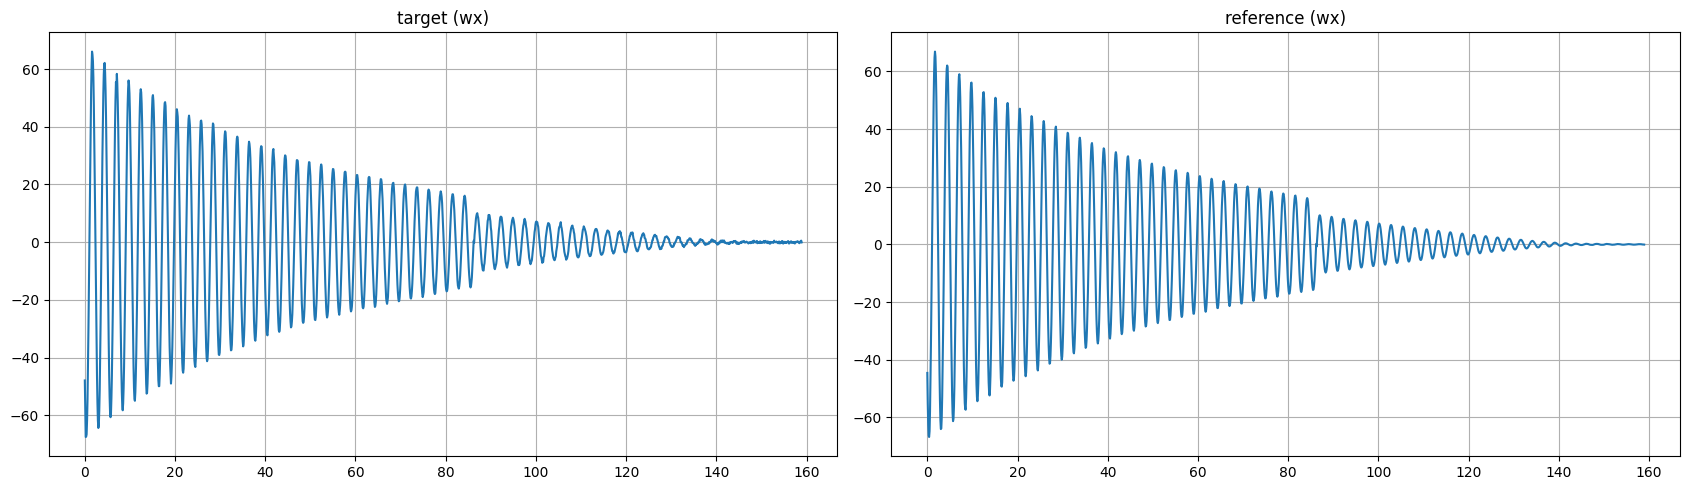
\includegraphics[width=0.47\linewidth]{imagens/V/comp0_.png}
        }

        \textbf{Fonte:} Autoria Própria
        \label{fig:comp0}
    \end{figure}

    A sobreposição das curvas de roll do DRMM e do Kongsberg MRU 5 (esquerda) demonstra que ambos os dispositivos respondem de forma praticamente idêntica às oscilações do pêndulo. A comparação espectral (direita) confirma que o DRMM preserva as mesmas componentes de frequência do sinal de referência sem amplificação ou atenuação seletiva, validando a qualidade dos filtros implementados e a adequação da frequência de corte adotada.

\subsection{Validação de Temperatura}

    Para verificar a estabilidade térmica em condições de campo, o DRMM foi monitorado continuamente durante 12 horas de operação, com o sensor KERNEL em funcionamento constante. O gráfico da \autoref{fig:temperatura} exibe a evolução da temperatura interna ao longo do tempo.

    \begin{figure}[!htbp]
        \centering
        \caption{Estabilidade das Medições com Variação de Temperatura}
        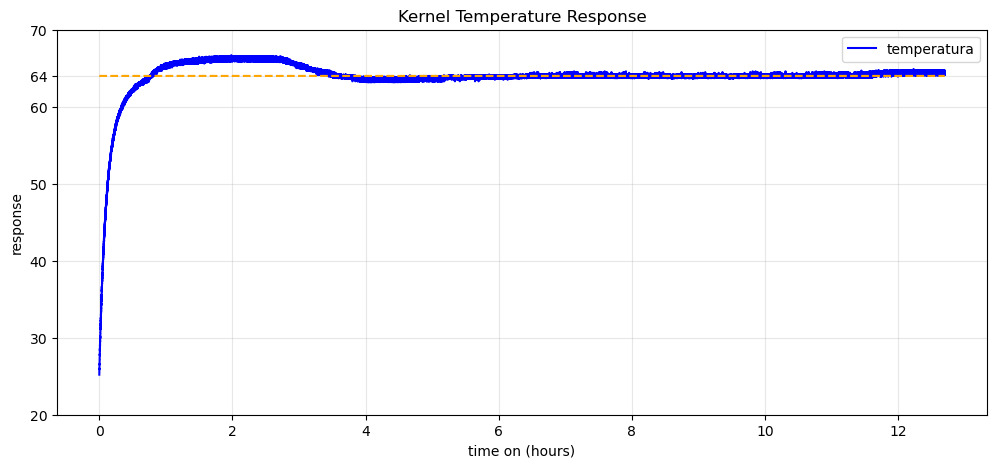
\includegraphics[width=0.82\linewidth]{imagens/V/temperatura.png}

        \textbf{Fonte:} Autoria Própria
        \label{fig:temperatura}
    \end{figure}

    Os resultados confirmam que, ao ativar o sistema, a temperatura interna parte do valor ambiente e sobe de forma exponencial à medida que o sensor KERNEL dissipa calor. A curva estabiliza em torno de 64$^\circ$C, dentro da faixa operacional dos componentes eletrônicos ($-$40$^\circ$C a $+$85$^\circ$C), sem atingir níveis críticos. Esse comportamento térmico controlado valida a eficácia do projeto de encapsulamento e confirma que a compensação interna de temperatura do KERNEL mantém a precisão das medições durante operação prolongada offshore.


%=============================================================================
\newpage
\section{Registros e Propriedade Intelectual}
%=============================================================================

Paralelamente ao desenvolvimento técnico, foram realizados os procedimentos de documentação técnica e registro de propriedade intelectual, consolidando os ativos do projeto e preparando o DRMM para eventual comercialização.

\subsection{Manuais de Instalação e Operação}

    Foi elaborado um manual de instalação abrangendo os procedimentos de montagem mecânica do dispositivo na estrutura offshore, a conexão elétrica dos cabos RS-422 e RS-232, a configuração dos parâmetros via protocolo RS-232 e a operação do aplicativo HMS para monitoramento e exportação de dados. O documento segue o padrão de manuais técnicos industriais, com seções de aviso de segurança, lista de materiais necessários, procedimento passo a passo e resolução de problemas comuns. Está disponível em repositório digital e acompanha o produto como entrega obrigatória.

\subsection{Desenhos Técnicos dos Circuitos}

    Os esquemáticos e os arquivos Gerber da PCB final foram gerados no Altium Designer e entregues em conjunto com o dispositivo. O circuito do sistema embarcado final é apresentado na \autoref{fig:circuito001}.

    \begin{figure}[!htbp]
        \centering
        \caption{Circuito Final do Sistema Embarcado DRMM}
        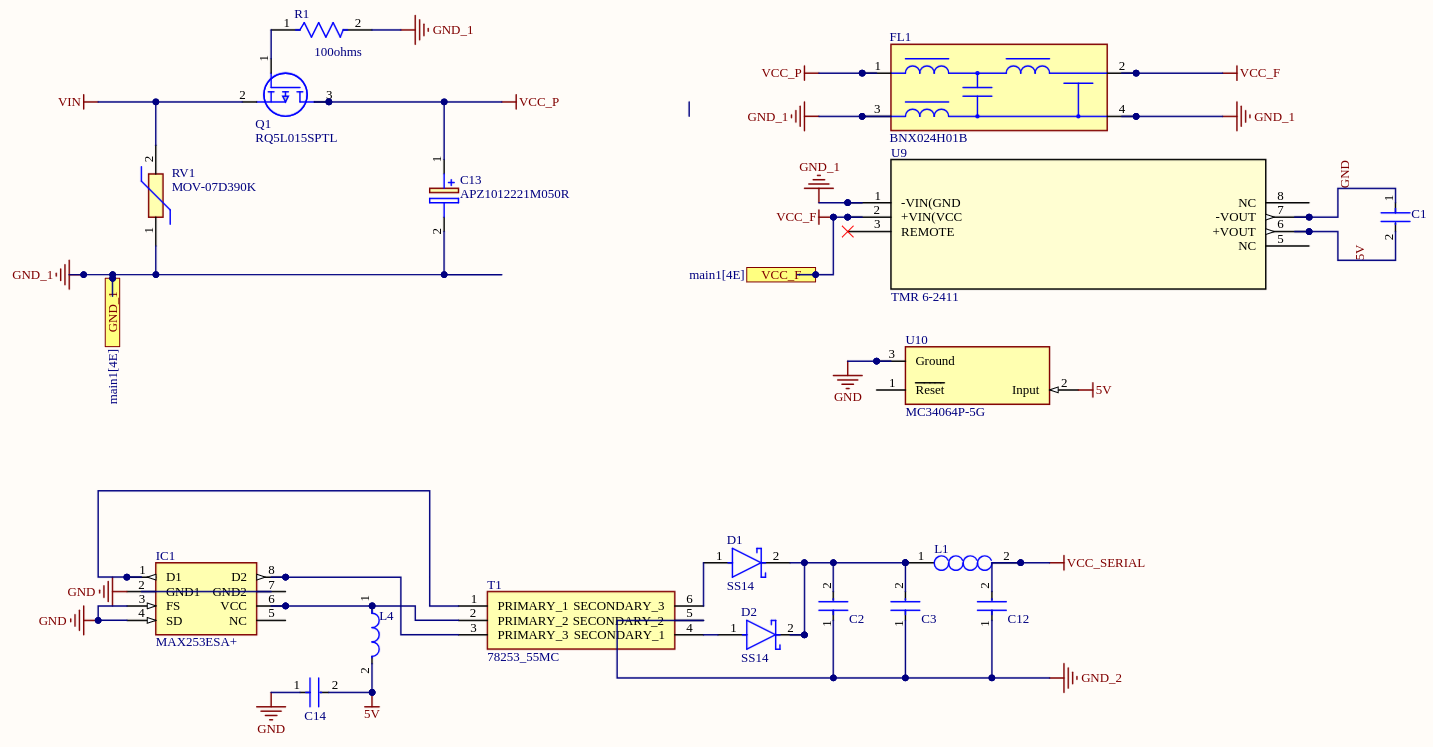
\includegraphics[width=.85\linewidth]{imagens/V/circuito01.png}

        \textbf{Fonte:} Autoria Própria
        \label{fig:circuito001}
    \end{figure}

    O esquemático apresenta as duas placas do sistema embarcado final em uma única folha, com destaque para o isolamento galvânico da interface RS-422 (obtido por optoacopladores) e o regulador de tensão LDO que mantém a alimentação do sensor KERNEL estável em 5 V com ripple inferior a 50 mV, mesmo com variações da fonte de alimentação entre 9 V e 36 V. Os arquivos Gerber gerados foram validados pelo fabricante Wego Sistemas antes da produção das placas.


\subsection{Registros de Software}

    Os softwares desenvolvidos foram registrados junto ao Instituto Nacional da Propriedade Industrial (INPI) para proteção dos ativos intangíveis do projeto. A \autoref{tab:hash} identifica cada software pela linguagem, framework e finalidade.

    \begin{table}[H]
        \centering
        \caption{Softwares do Projeto e Respectivas Identificações}
        \label{tab:hash}
        \vspace{-0.2cm}

        \small
        {\renewcommand{\arraystretch}{1.5}
        \begin{longtable}{|m{3.5cm}|m{5cm}|m{5.5cm}|}
        \hline
            \centering\textbf{Software} & \centering\textbf{Tecnologia} & \centering\textbf{Finalidade}\arraybackslash \\
        \hline
            Firmware DRMM & C++ / Arduino (ESP32-S3) & Aquisição, filtragem e transmissão de dados \\
        \hline
            HMS Interface & Tauri + React + Rust & Monitoramento e configuração via desktop \\
        \hline
            Algoritmos de Filtragem & Python 3 (NumPy, SciPy) & Prototipagem e validação dos filtros \\
        \hline
        \end{longtable}}

        \small
        \textbf{Fonte:} Autoria Própria
    \end{table}

    O registro dos três softwares junto ao INPI confere proteção de 50 anos sobre o código-fonte, garantindo que a implementação dos algoritmos de filtragem e fusão sensorial, bem como a interface HMS, sejam ativos protegidos da empresa. Isso é um diferencial competitivo relevante para futuros processos de licenciamento ou transferência de tecnologia.

\newpage
\subsection{Certificado de Calibração}

    Ao término de cada sessão de calibração, o sistema gera automaticamente um certificado contendo os coeficientes de calibração aplicados, as métricas de erro ($R^2$, RMSE e desvio padrão residual), as condições ambientais do ensaio e a data de validade recomendada para recalibração.

    \begin{figure}[H]
        \centering
        \caption{Certificado de Calibração}

        \subfloat[Modelo Kongsberg]{
            \frame{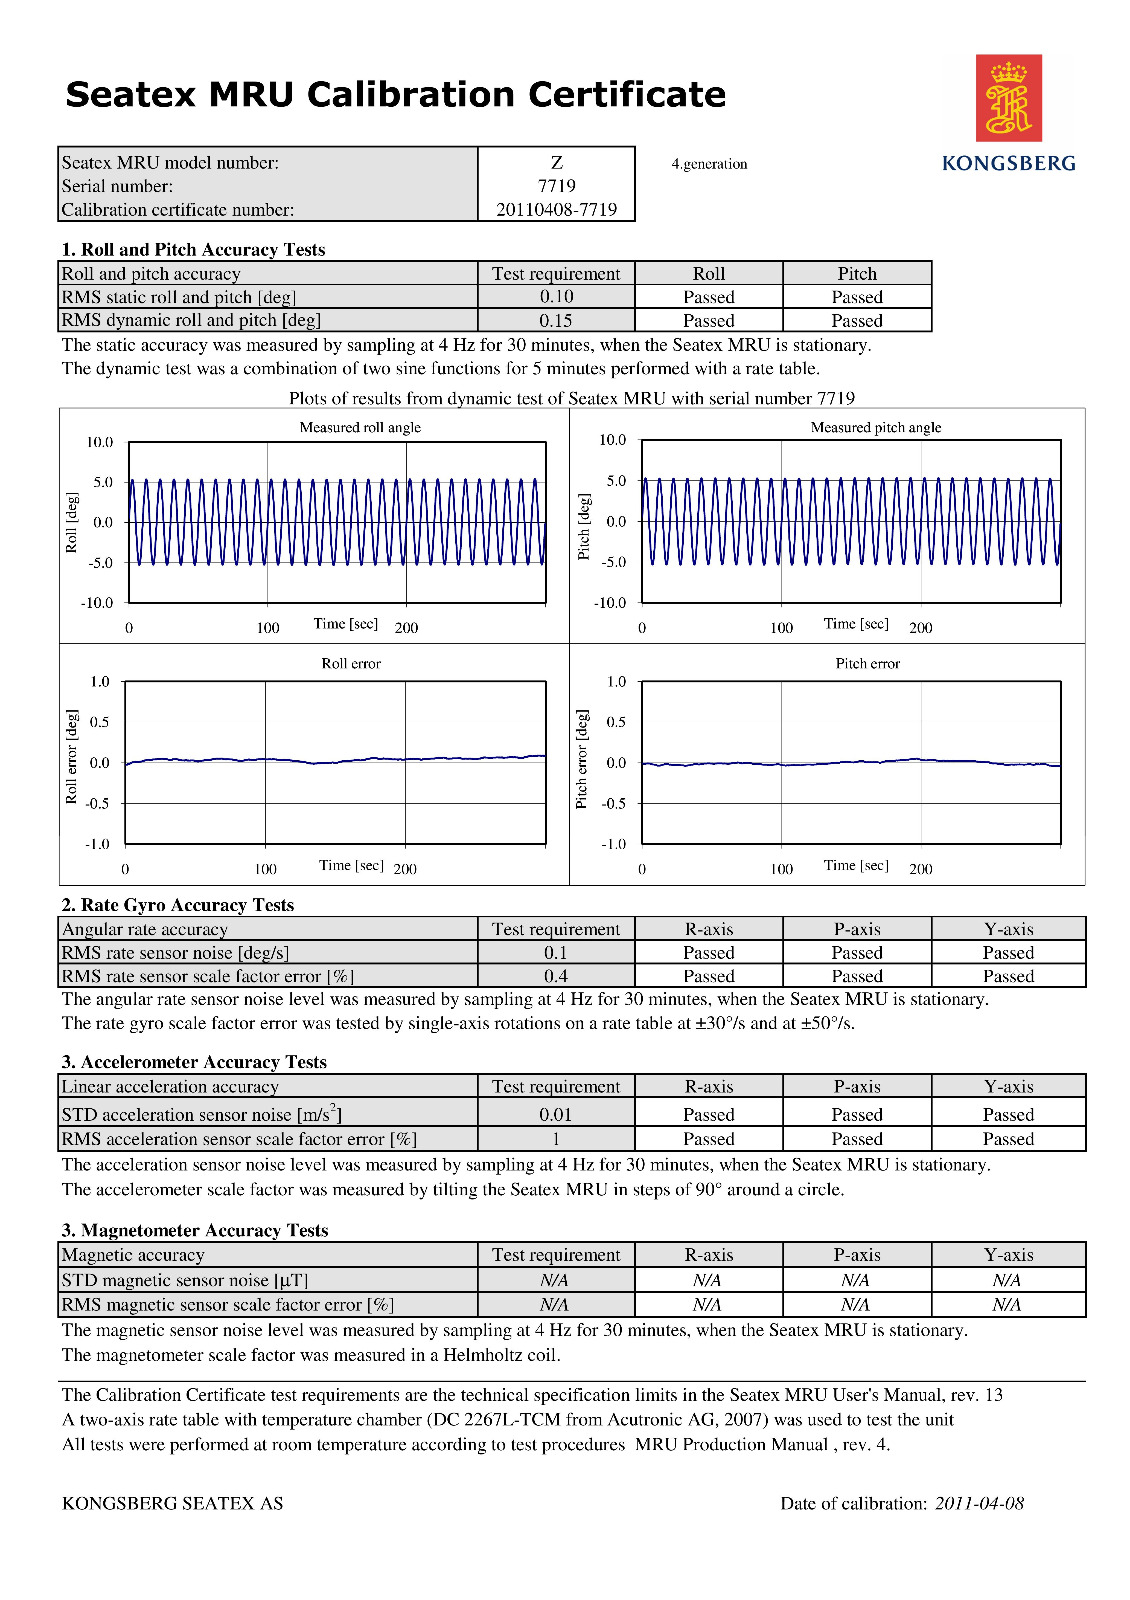
\includegraphics[height=11.4cm]{imagens/V/kongsberg_certificado.png}}
        }\hfill
        \subfloat[Modelo Measure]{
            \frame{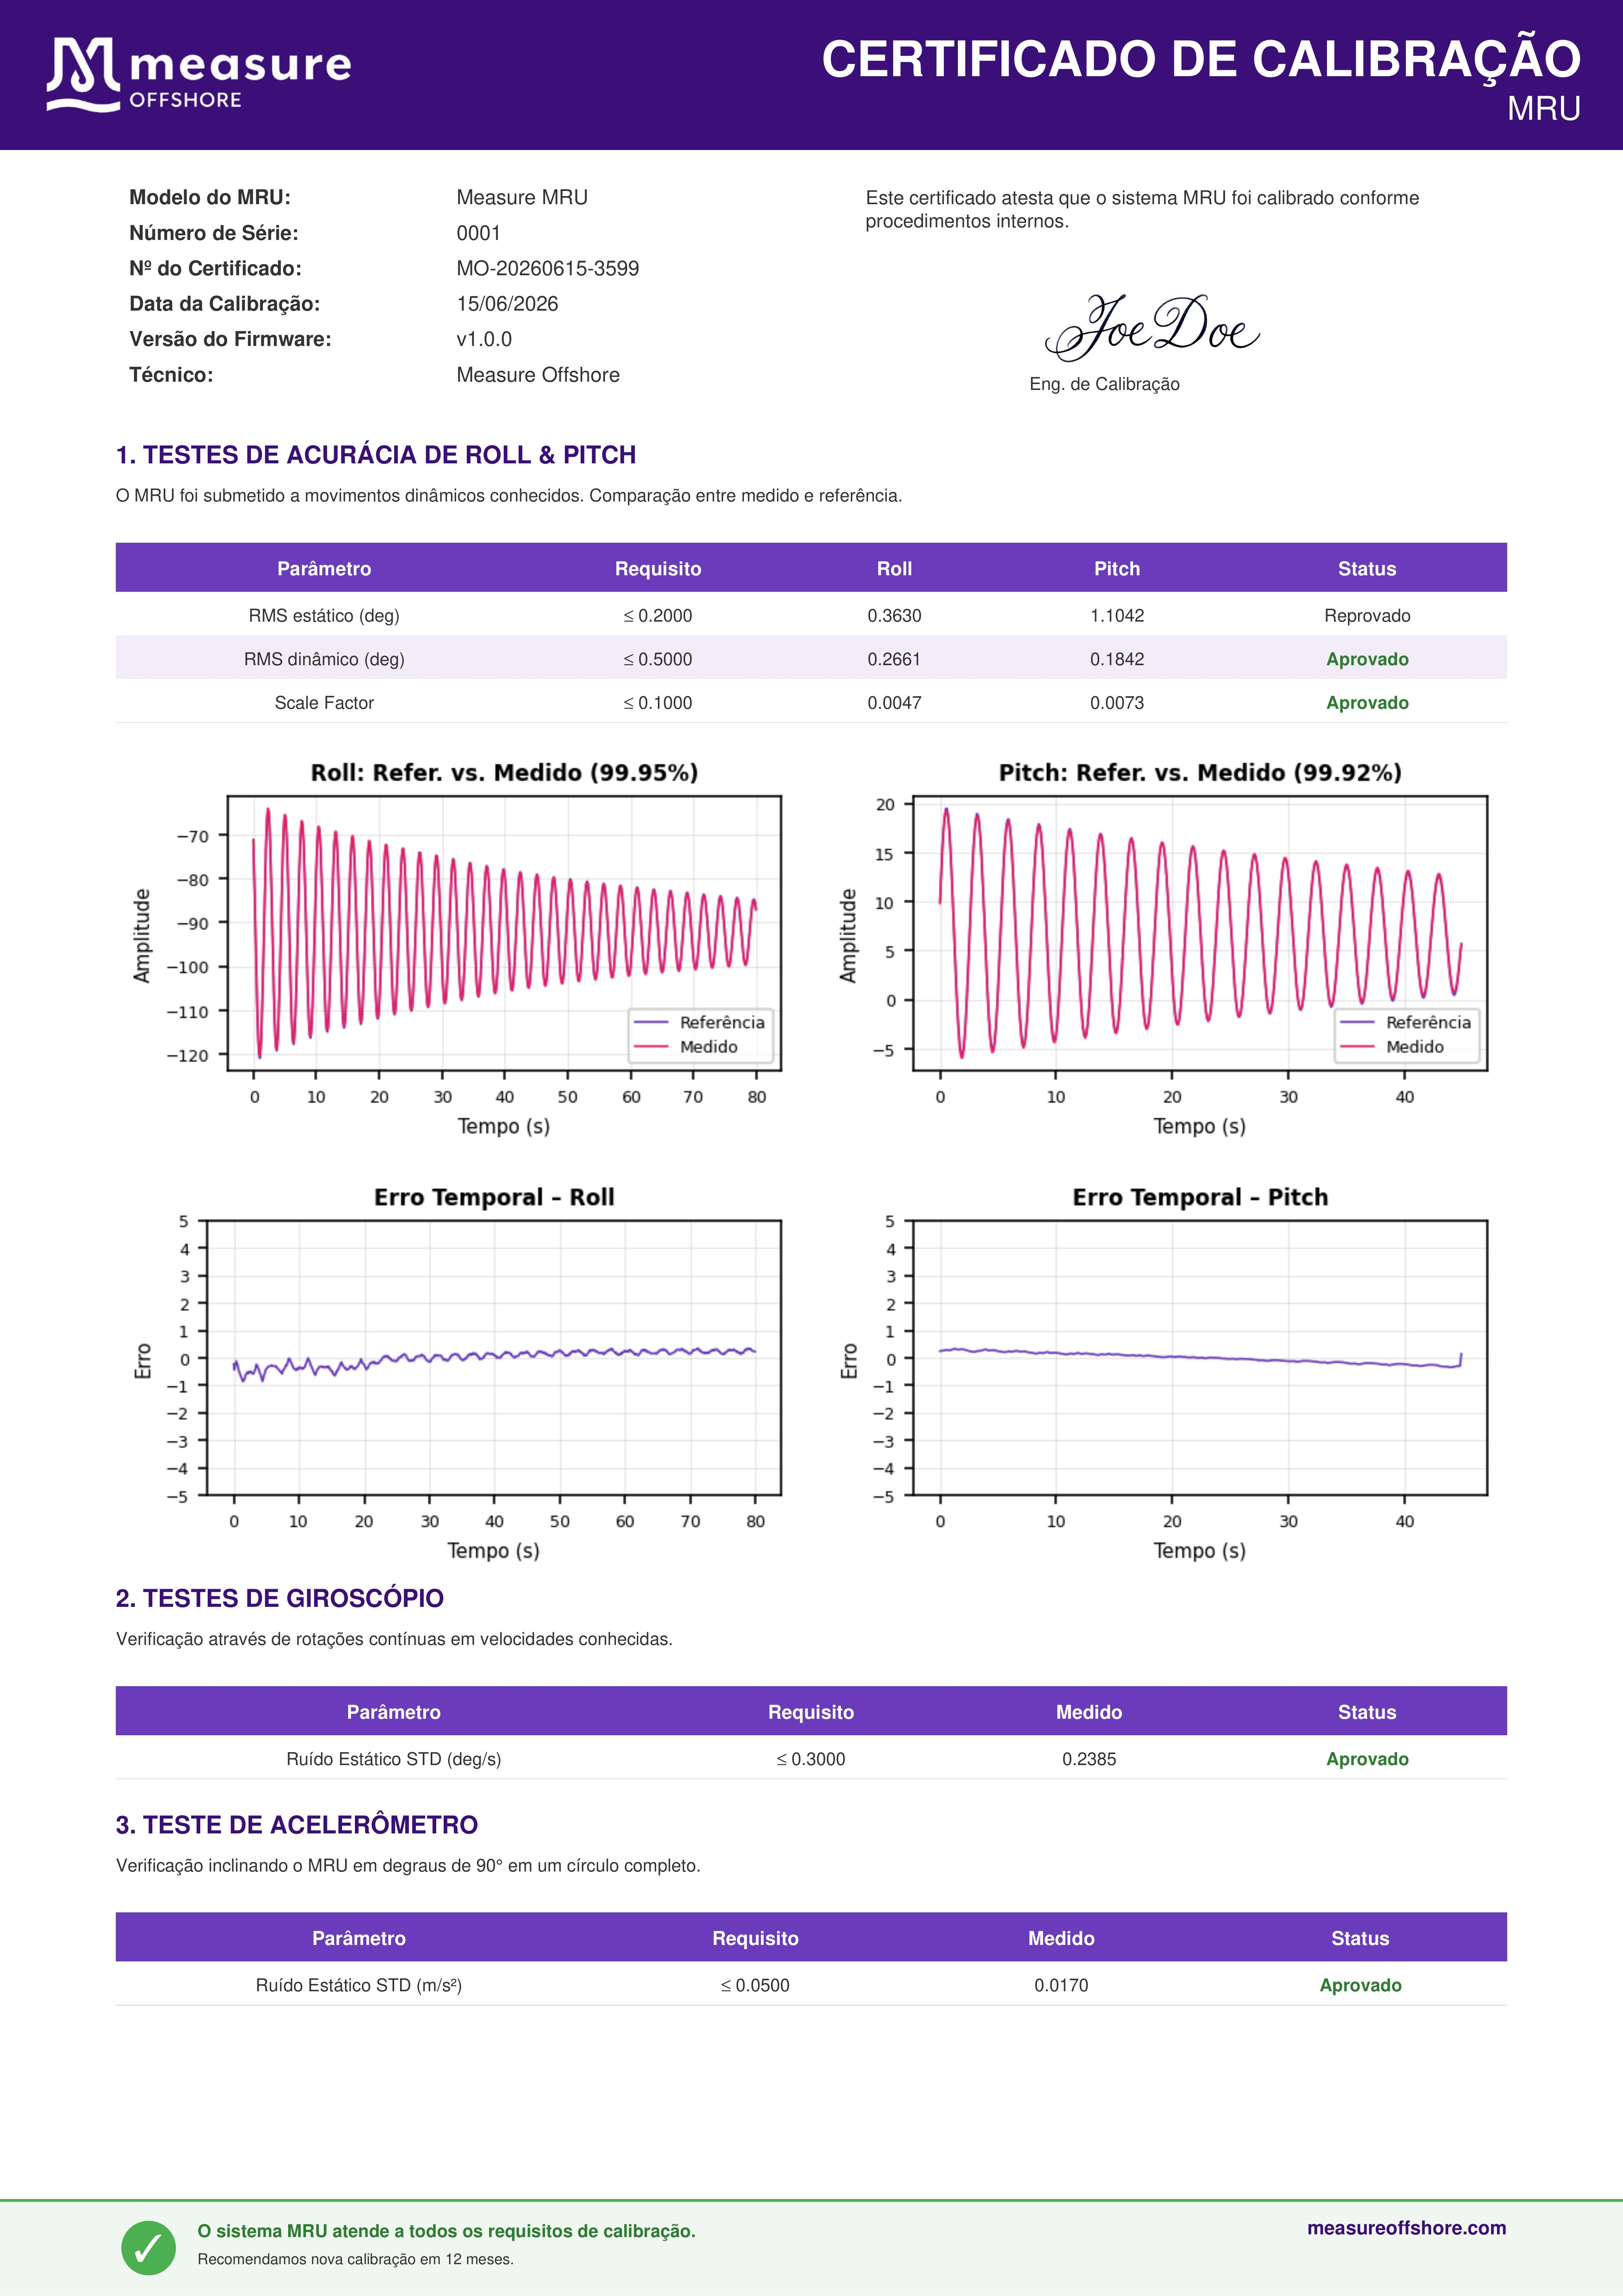
\includegraphics[height=11.4cm]{imagens/V/img_1.png}}
        }
        
        \textbf{Fonte:} Autoria Própria
        \label{fig:certificado}
    \end{figure}

    O certificado emitido pelo HMS contém os campos de identificação do dispositivo, os coeficientes de calibração calculados, as métricas de qualidade do ajuste e a data de validade da calibração. A versão digital é armazenada no banco de dados do HMS e pode ser exportada em formato PDF para arquivamento técnico ou apresentação em auditorias de conformidade com a NORMAM-27/DPC.


%=============================================================================
\newpage
\section{Próximos Passos}
%=============================================================================

Os resultados obtidos validam a viabilidade técnica do DRMM, mas também apontam oportunidades de aprimoramento que constituem a agenda de desenvolvimento das etapas seguintes.

\subsection{Mesa de Calibração Motorizada de Dois Eixos}

    O principal limitante atual da calibração é o pêndulo de eixo único, que permite reproduzir apenas movimentos de roll de forma controlada. Para calibrar o eixo de pitch com igual rastreabilidade e automatizar o processo, está em desenvolvimento uma mesa de calibração motorizada de dois eixos, ilustrada na Figura~\ref{fig:mesa_motor}.

    \begin{figure}[!htbp]
        \centering
        \caption{Mesa de Calibração Motorizada de Dois Eixos (Projeto em Desenvolvimento)}

        \subfloat[Vista isométrica]{
            \frame{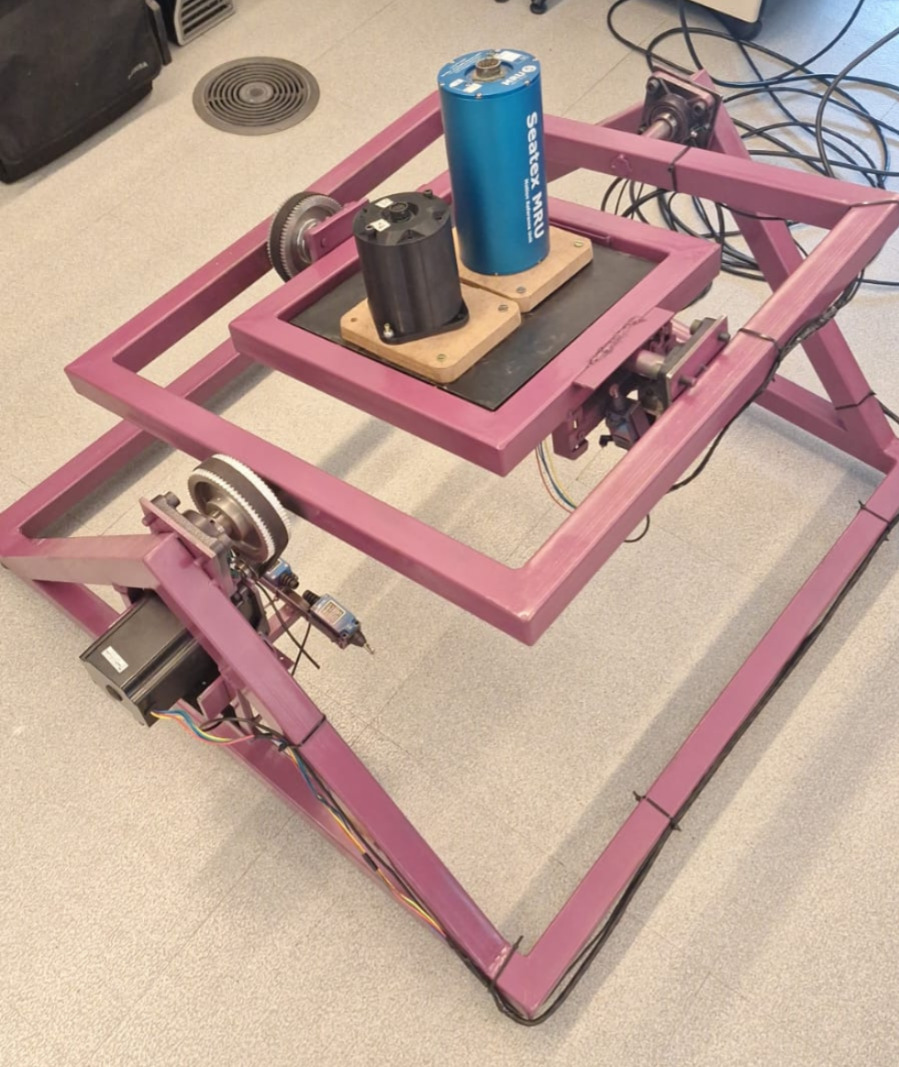
\includegraphics[height=5cm]{imagens/V/mesa1.png}}
        }\hspace{0.5cm}
        \subfloat[Modelo 3D detalhado]{
            \frame{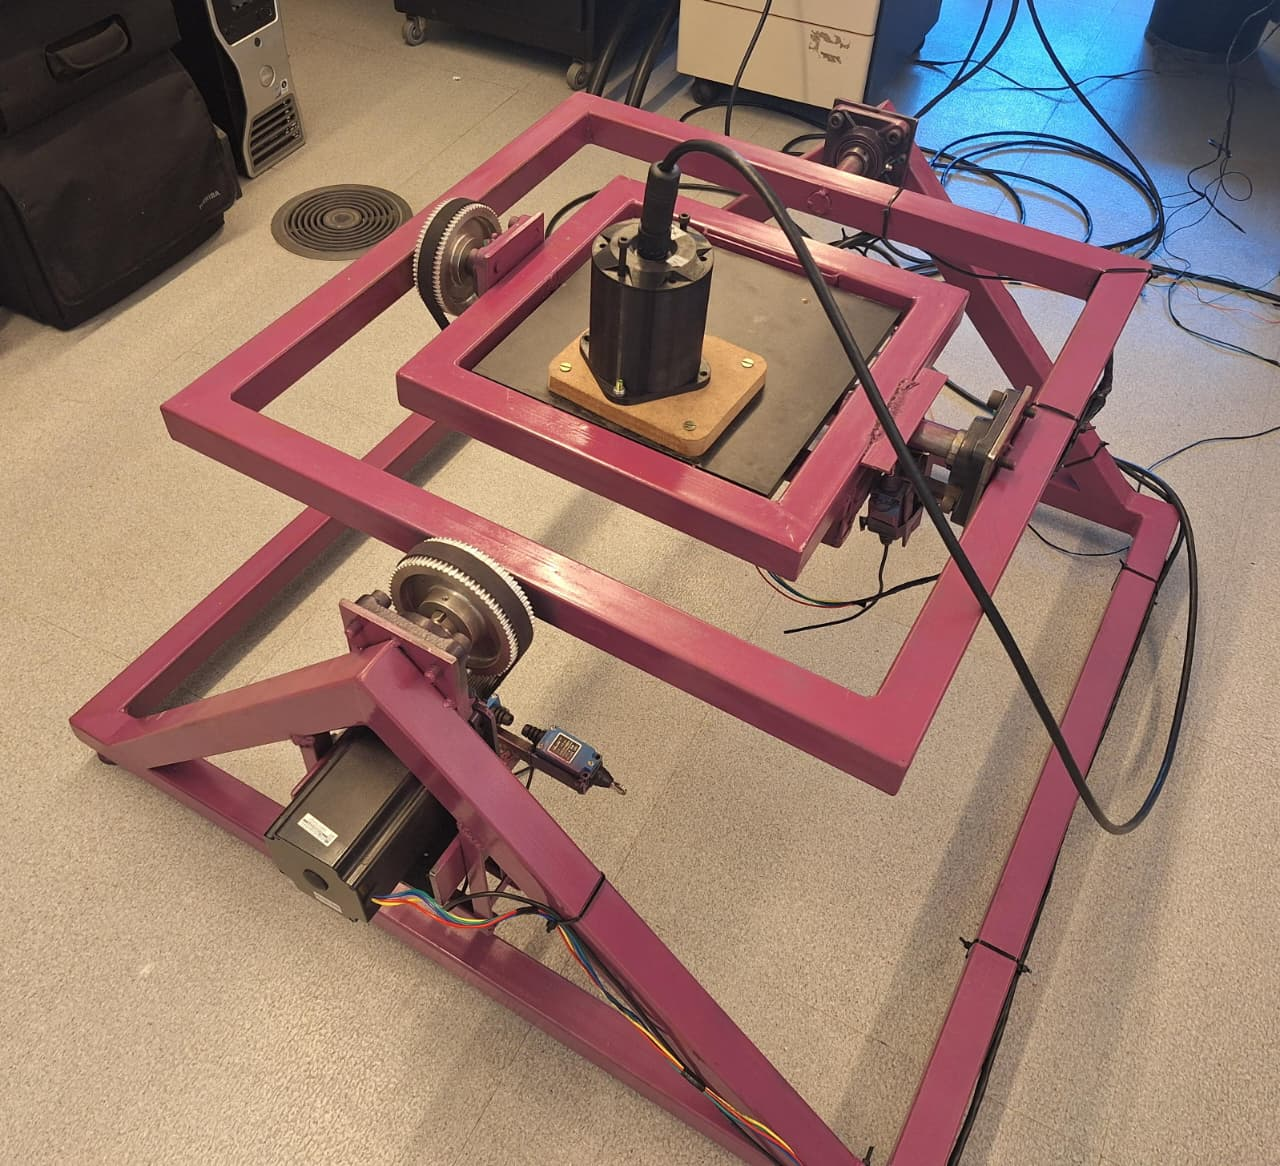
\includegraphics[height=5cm]{imagens/V/mesa2.png}}
        }

        \textbf{Fonte:} Autoria Própria
        \label{fig:mesa_motor}
    \end{figure}

    A mesa incorporará motores de passo de alta resolução com controle por microcontrolador dedicado, permitindo programar perfis de movimento padronizados com amplitude, velocidade e perfil temporal definidos. A arquitetura de dois eixos independentes permite calibrar roll e pitch sequencialmente sem necessidade de remontar o dispositivo, reduzindo o tempo total de calibração de dois procedimentos separados para uma única sessão.

\subsection{Aprimoramentos no Firmware}

    Três linhas de melhoria foram identificadas para o firmware. A primeira é a implementação de servidor HTTP embarcado para configuração remota via navegador web, eliminando a necessidade do cabo RS-232. A segunda é a compensação de temperatura em tempo real com modelo polinomial ajustado a partir dos dados de calibração, visando reduzir a deriva em temperatura para níveis inferiores a 0,01$^\circ$/$^\circ$C. A terceira é a validação dos modelos de aprendizagem de máquina para fusão sensorial em um coprocessador dedicado, explorando os resultados promissores descritos na Seção 4.


%=============================================================================
\newpage
\section{Conclusão}
%=============================================================================

O presente relatório final integrou e consolidou o desenvolvimento do Dispositivo de Referência de Monitoramento dos Movimentos (DRMM), apresentando de forma coesa a trajetória técnica que partiu da pesquisa de componentes e chegou à validação experimental de um protótipo funcional de tecnologia nacional.

A pesquisa e comparação sistemática de MRUs comerciais, módulos IMU e sensores MEMS estabeleceu os requisitos de desempenho e conduziu à seleção do sensor Inertial Labs KERNEL-110/120 como núcleo inercial do DRMM. A modelagem matemática dos filtros digitais demonstrou que a combinação por Covariance Intersection produz estimativas robustas mesmo com sensores de custo reduzido. A representação de atitude por quaternions eliminou as singularidades de Gimbal Lock, tornando o algoritmo numericamente estável para qualquer orientação do dispositivo.

O hardware evoluiu por três gerações de PCBs, cada uma aprimorando a robustez elétrica e reduzindo as dimensões para adequação ao compartimento cilíndrico metálico com proteção IP67. O firmware em C++ sobre ESP32-S3 Mini executa o ciclo de aquisição, filtragem e transmissão NMEA 0183 a 38400 baud em tempo real, com configuração in loco via RS-232. O aplicativo HMS em Tauri com Rust e React completa a solução como interface de monitoramento e armazenamento de dados, sendo registrado junto ao INPI como ativo de propriedade intelectual do projeto.

A calibração com pêndulo e encoder rotativo de 5000 PPR ($0{,}072^\circ$/pulso) produziu coeficiente de determinação $R^2 = 0{,}9995$, confirmando a linearidade do sensor e a eficácia do protocolo de calibração. A comparação com o Kongsberg MRU 5 evidenciou precisão estática equivalente (0,03$^\circ$ RMS) e interface de comunicação idêntica. O monitoramento térmico de 12 horas confirmou estabilização interna em torno de 64$^\circ$C, dentro da faixa operacional dos componentes, validando o projeto de encapsulamento e a operação prolongada offshore.

Conclui-se, portanto, que o DRMM atingiu os objetivos estabelecidos, entregando um sistema embarcado nacional com desempenho equivalente ao dos equipamentos importados de referência, a um custo de produção estimado em até 60\% inferior. Os trabalhos futuros, centrados na mesa de calibração motorizada de dois eixos, na compensação de temperatura embarcada e na expansão para outros segmentos navais, apontam para um caminho claro de consolidação técnica e de crescimento comercial sustentável.

%=============================================================================
\newpage

\bibliography{references}
%=============================================================================

\end{document}
